\section{Construction of template distributions}
There were no selection criteria found to make a clear rejection of the background events without sacrificing a significant amount of signal. For this reason, a multivariate approach using Boosted Decision Trees that combines several discriminating variables in the TMVA framework is used. For the training, the BDTs are trained against all backgrounds, where the \NPL\ background is not taken into account. The BDT settings  avoid over-training and  maintain a good discriminating power against all backgrounds. The background and signal yields follow the relative fractions predicted by the simulation. 


The variables used to construct the BDTs include the angles, distances, masses and transverse momenta:
\begin{enumerate}
	\item pseudo rapidity of the SM top: TT+ST \Zut  , ST \Zct 
	\item invariant mass of the W lepton and the SM b jet: TT+ST \Zut , TT+ST \Zct\ 
	\item $\Delta \Phi$ between the W lepton and the SM b jet: TT+ST \Zut , ST \Zct\ 
	\item minimal $\Delta R$ between the W lepton and jets: TT \Zut 
	\item invariant mass of the Z boson: TT \Zut , TT \Zct\ 
	\item $\Delta \Phi$ between the W lepton and the Z boson: TT+ST \Zut , TT \Zct\ 
	\item $\Delta R$ between the W lepton and the SM b jet: TT+ST \Zut , TT \Zct\ 
	\item  number of CSVv2 medium WP b jets: TT \Zut , TT \Zct\ 
	\item invariant mass of the FCNC top: TT \Zut , TT \Zct\ 
	\item $\Delta R$ between the Z boson and the FCNC light jet: TT \Zut , TT \Zct\ 
	\item $\Delta R$ between the FCNC light jet and the SM b jet: TT \Zut , TT \Zct\ 
	\item charge of the W lepton times the absolute pseudo rapidity of the W lepton: ST \Zut 
	\item b discriminant of the highest $p_T$ jet: ST \Zut , ST \Zct\ 
	\item total Ht of the leptons: ST \Zut 
	\item the $p_T$ of the W lepton times its charge: ST \Zut 
	\item total invariant mass of the leptons: ST \Zct\ 
	\item $\Delta R$ between the W lepton and Z boson: TT+ST \Zct\ 
	\item total invariant mass of the event: TT \Zct\ 
	\item b discriminant of the FCNC light jet: TT \Zct\ 
	\item $\Delta R$ between the SM b jet and Z boson: TT \Zct\ 
\end{enumerate}
The pre fit distributions of the variables used for creating the multivariate discriminator are given in \Sec{sec:BDTvars}. The resulting multivariate discriminator are shown in \Sec{sec:BDTs}. 

\subsection{Distributions of the BDT variables}
\label{sec:BDTvars}
\todo{include distributions of the vars}


\subsection{BDTs}
\label{sec:BDTs}
\todo{better to do normalised? }
\begin{figure}[htbp]
	\centering
	% % 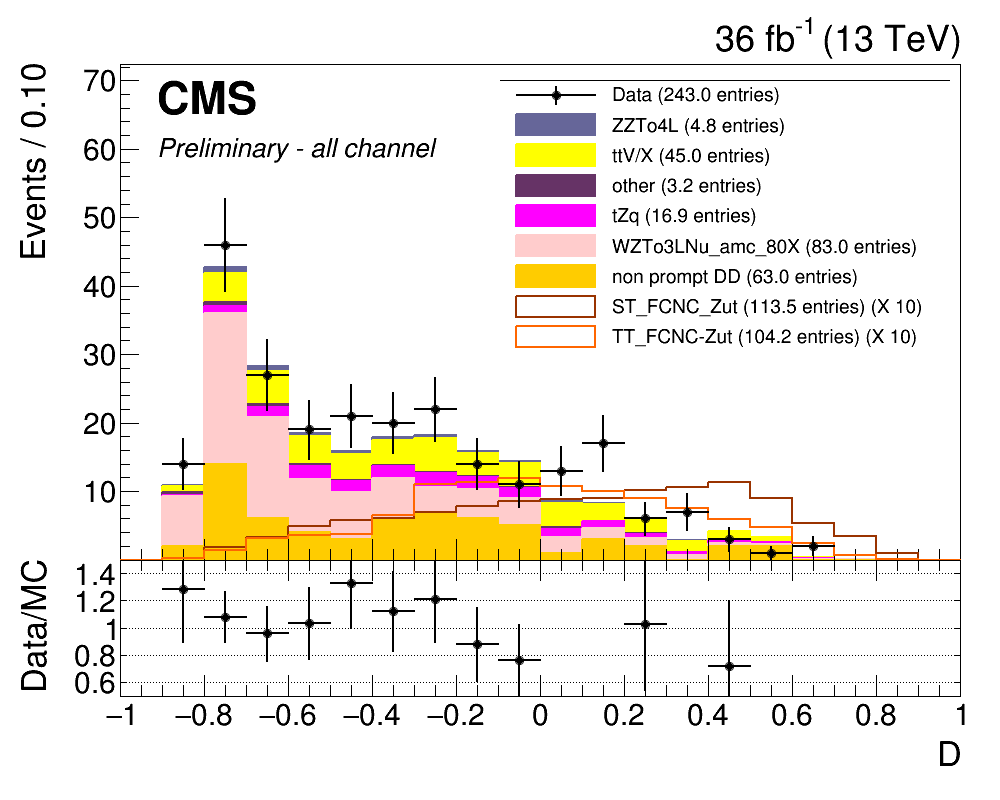
\includegraphics[width=0.47\linewidth]{FiguresAfterUnblinding/BDTunweighted//toppair_Zut_BDT_all_Stack}
	% % 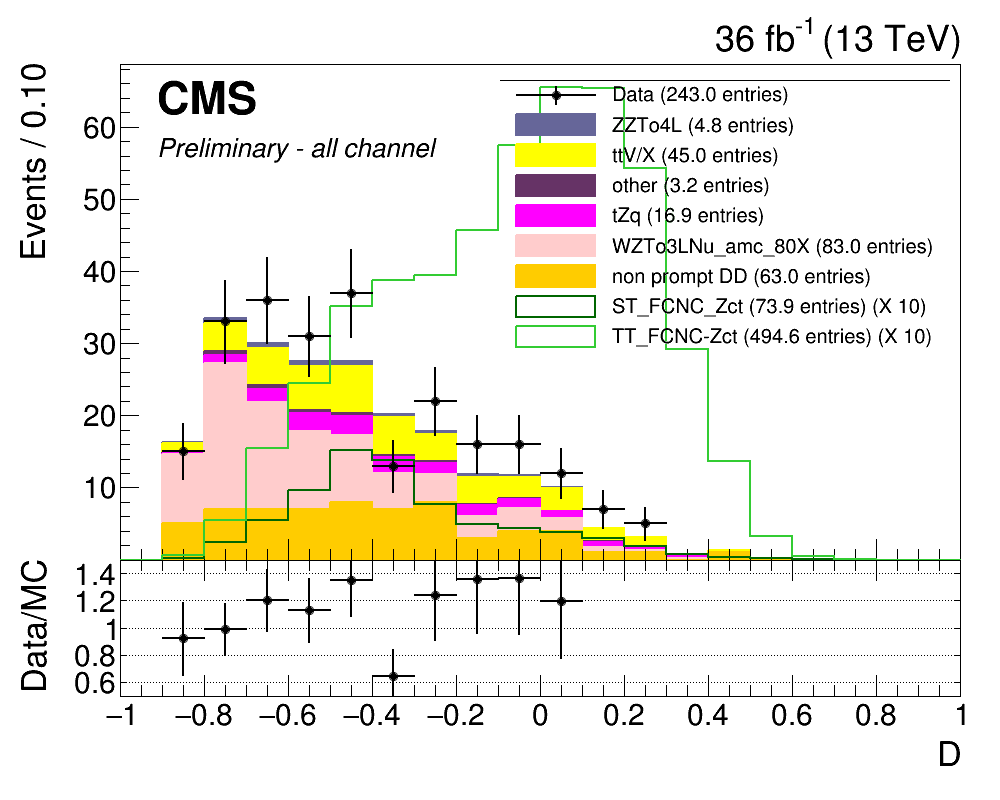
\includegraphics[width=0.47\linewidth]{FiguresAfterUnblinding/BDTunweighted//toppair_Zct_BDT_all_Stack}
	% % 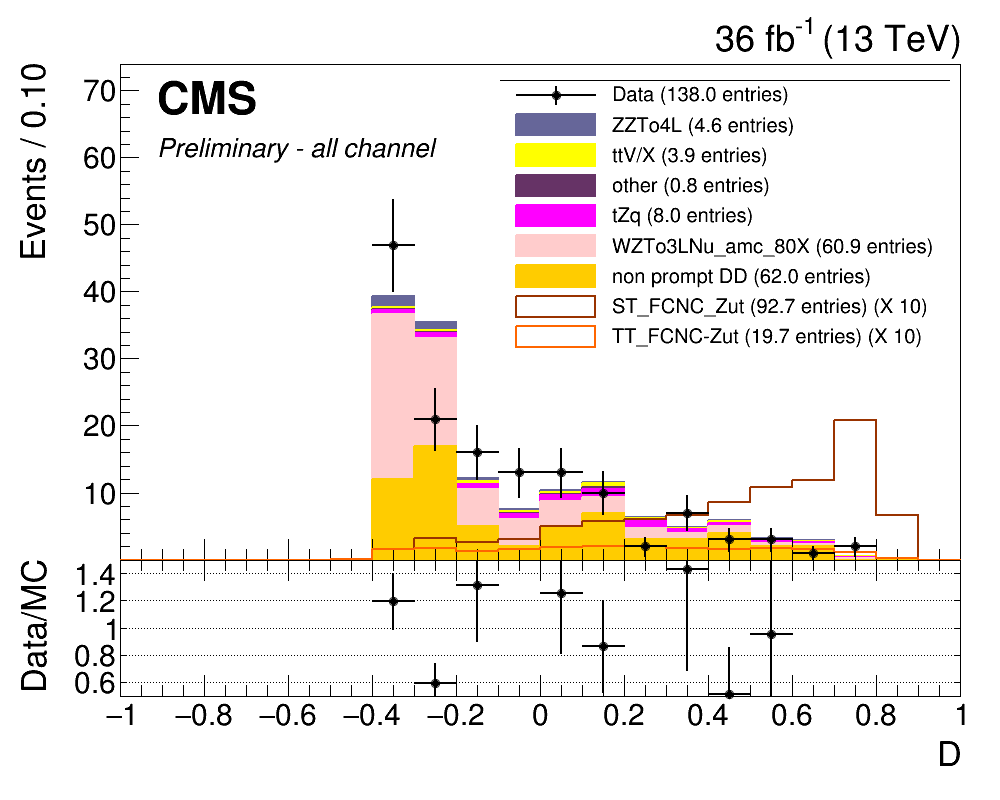
\includegraphics[width=0.47\linewidth]{FiguresAfterUnblinding/BDTunweighted//singletop_Zut_BDT_all_Stack}
	% % 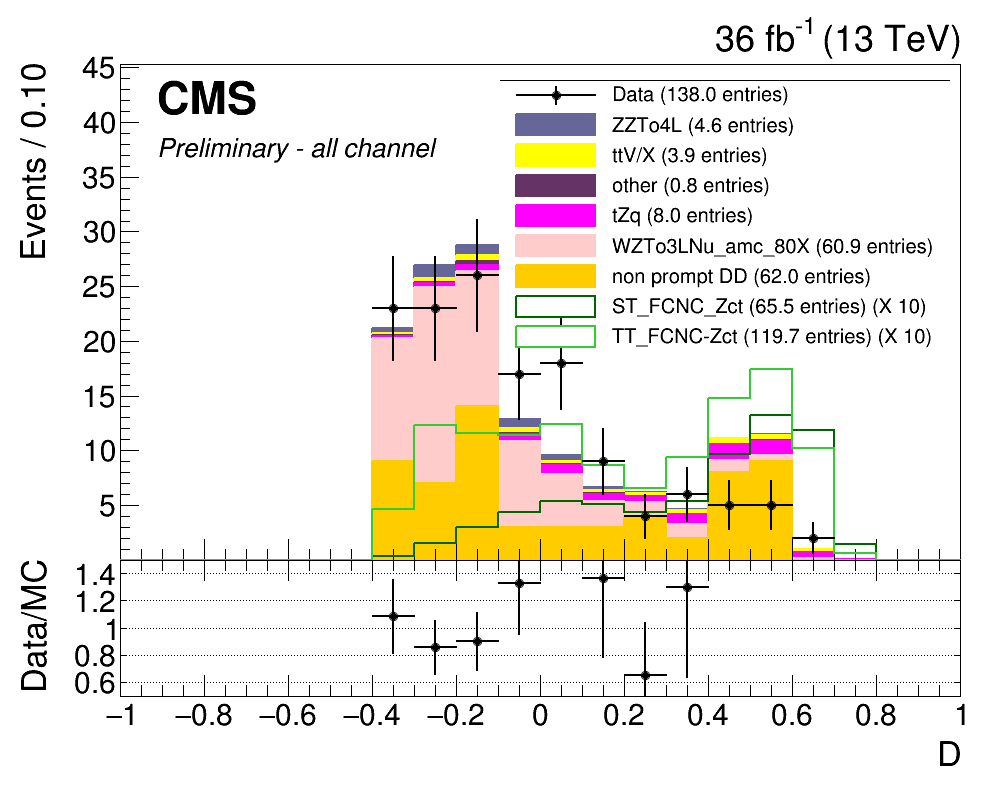
\includegraphics[width=0.47\linewidth]{FiguresAfterUnblinding/BDTunweighted//singletop_Zct_BDT_all_Stack}
	\caption{Distributions of the discriminating variable before the fit, all different leptonic channels together. Upper left: \TTSR\ \Zut , upper right: \TTSR\ \Zct ; lower left: \STSR\  \Zut , lower right: \STSR\  \Zct .}
	\label{fig:bdtallstack}
\end{figure}	

\begin{figure}[ht]
	\centering
	% % 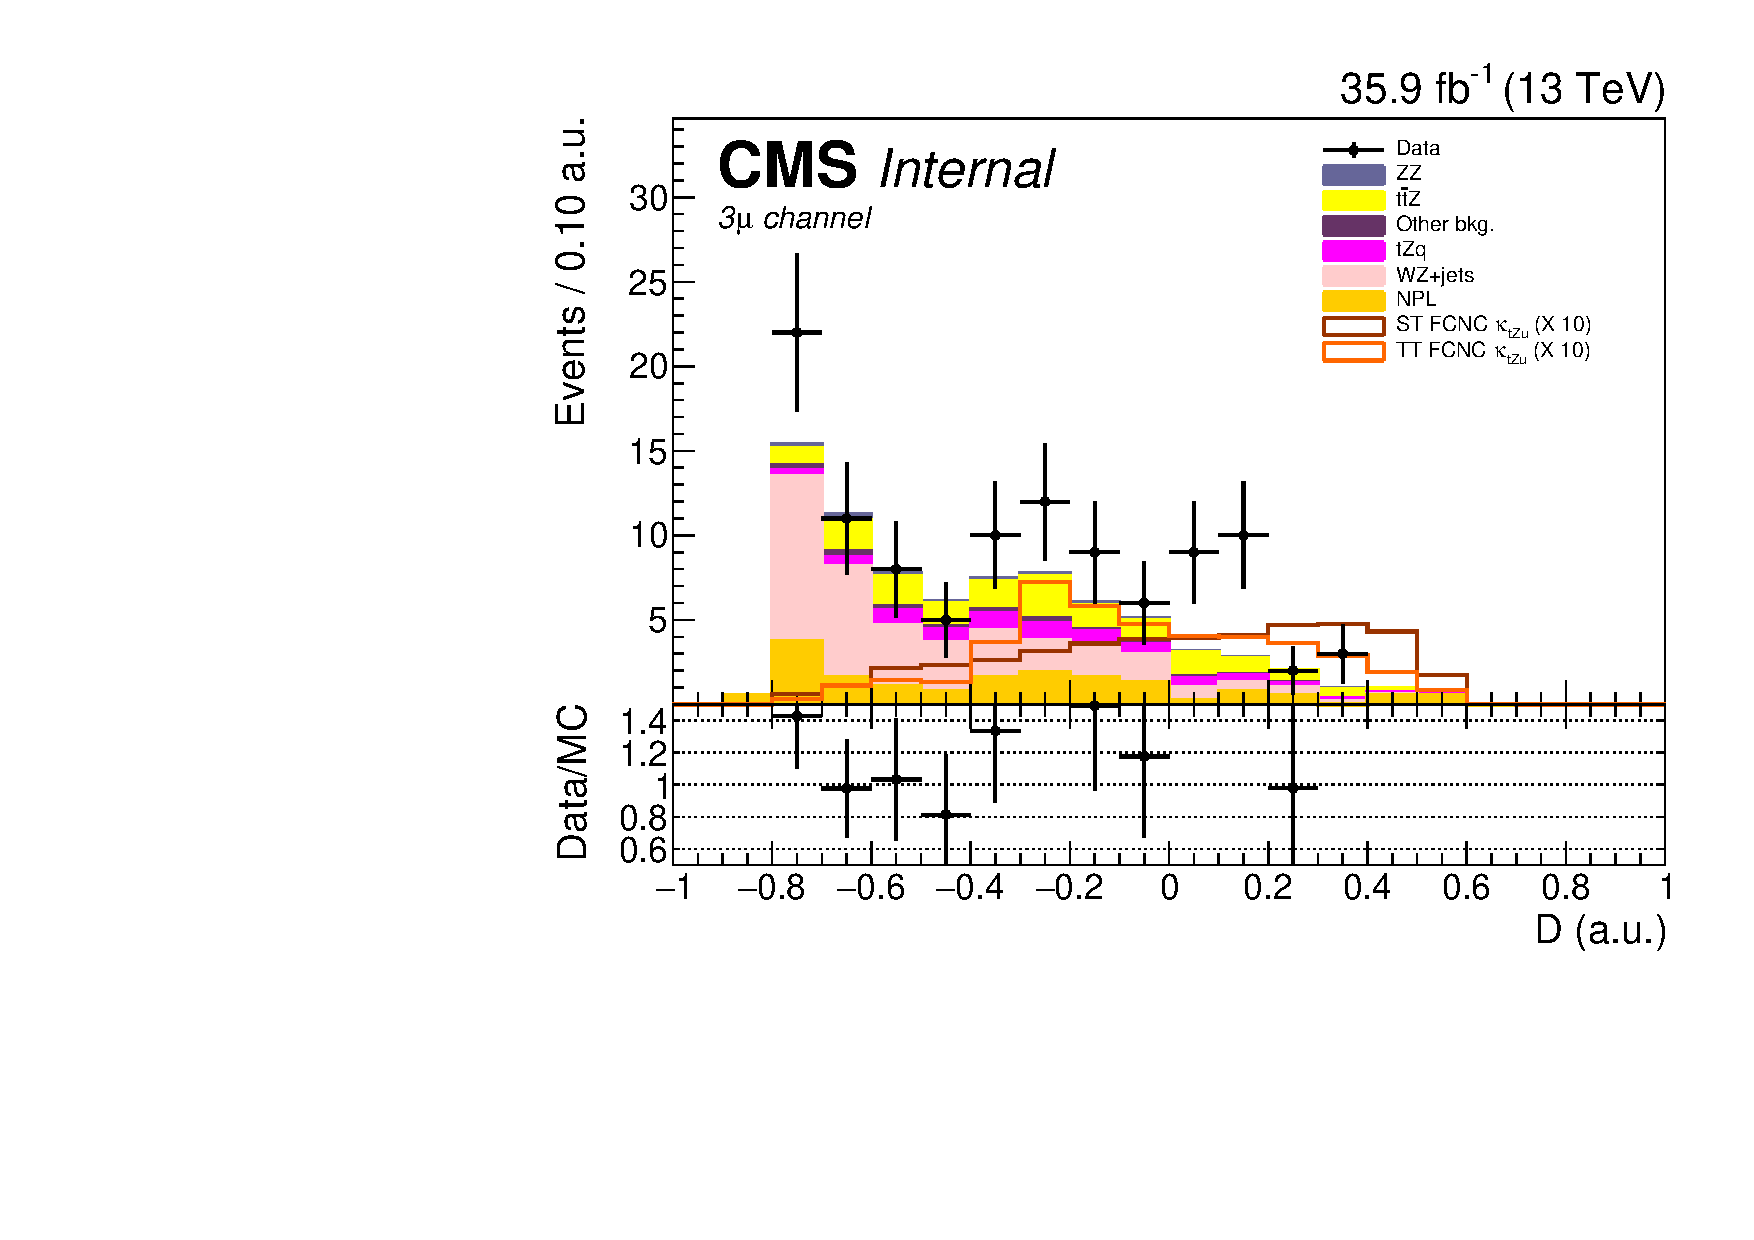
\includegraphics[width=0.47\linewidth]{FiguresAfterUnblinding/BDTunweighted//toppair_Zut_BDT_uuu_Stack}
	% % 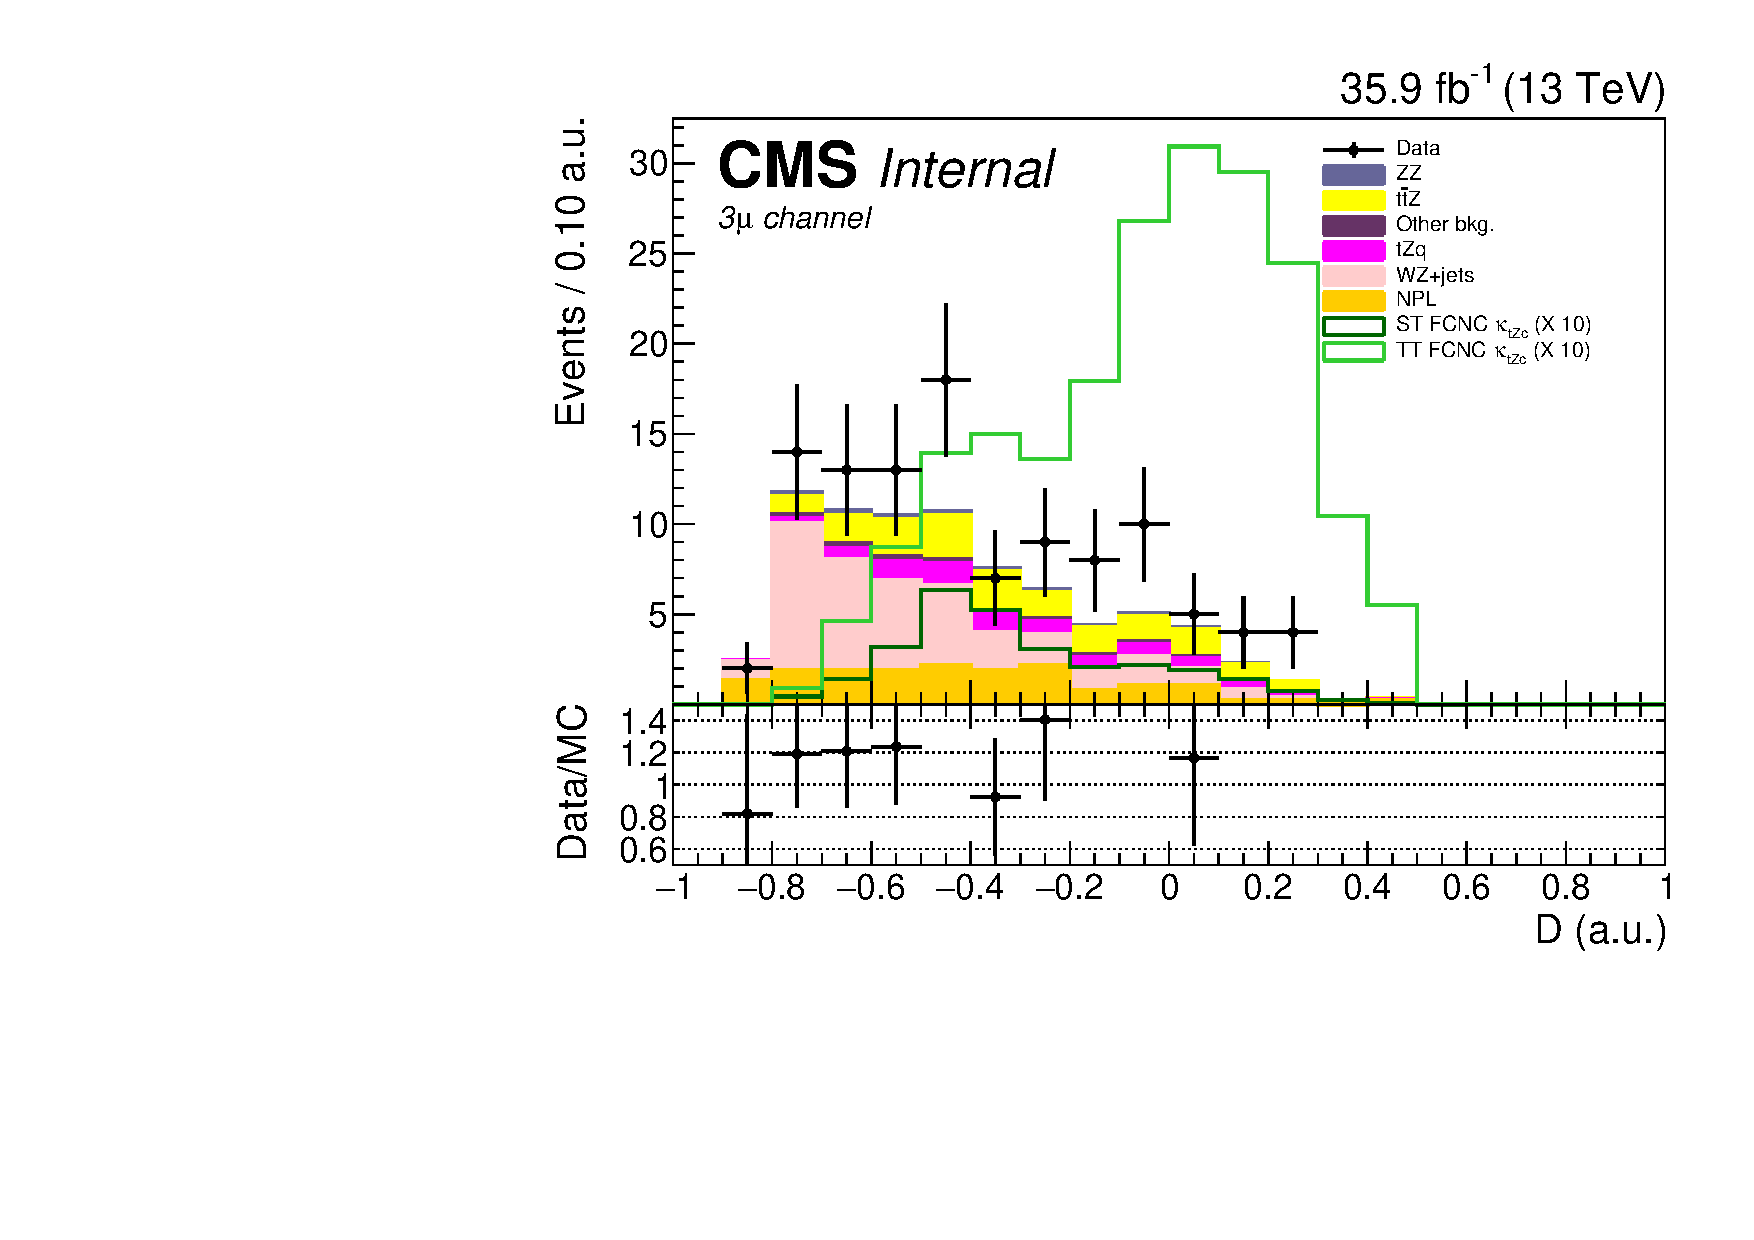
\includegraphics[width=0.47\linewidth]{FiguresAfterUnblinding/BDTunweighted//toppair_Zct_BDT_uuu_Stack}
	% % 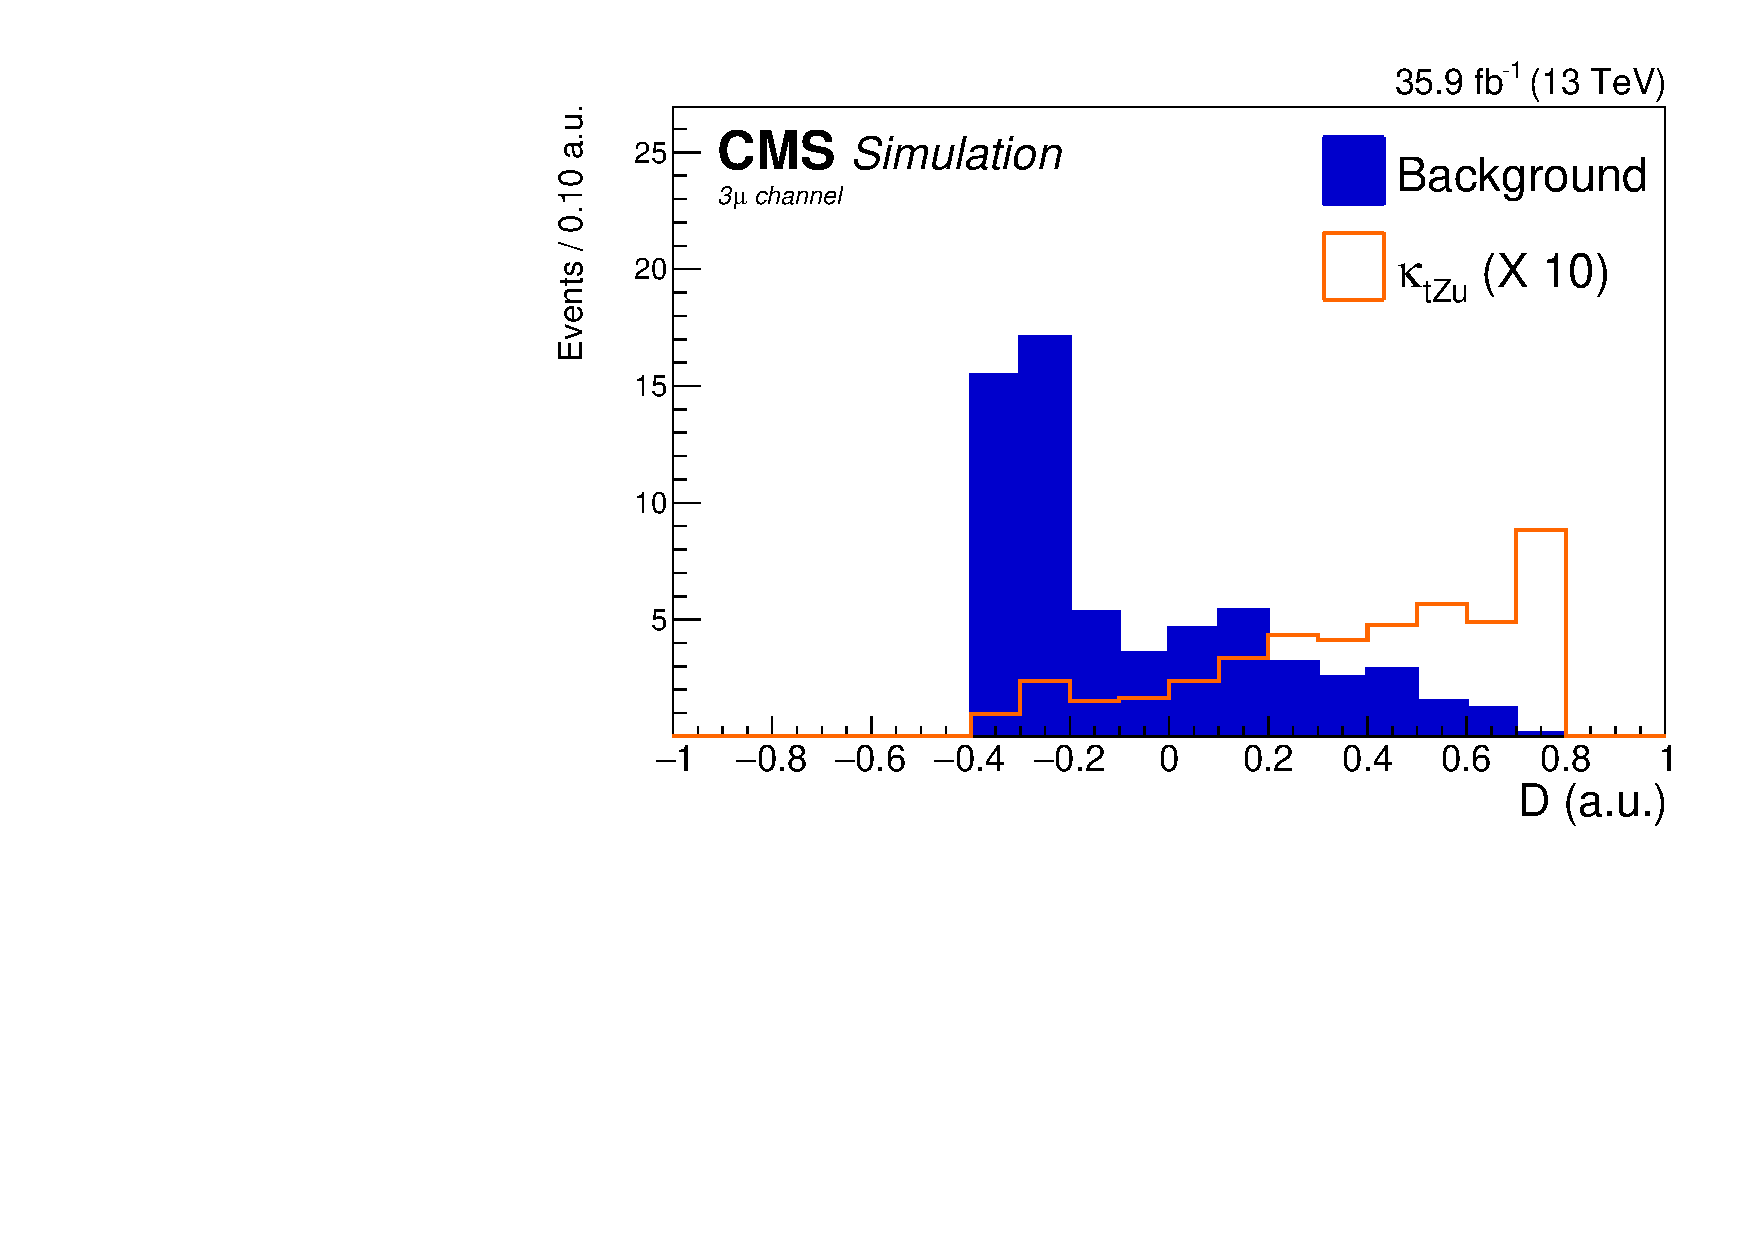
\includegraphics[width=0.47\linewidth]{FiguresAfterUnblinding/BDTunweighted//singletop_Zut_BDT_uuu_Stack}
	% % 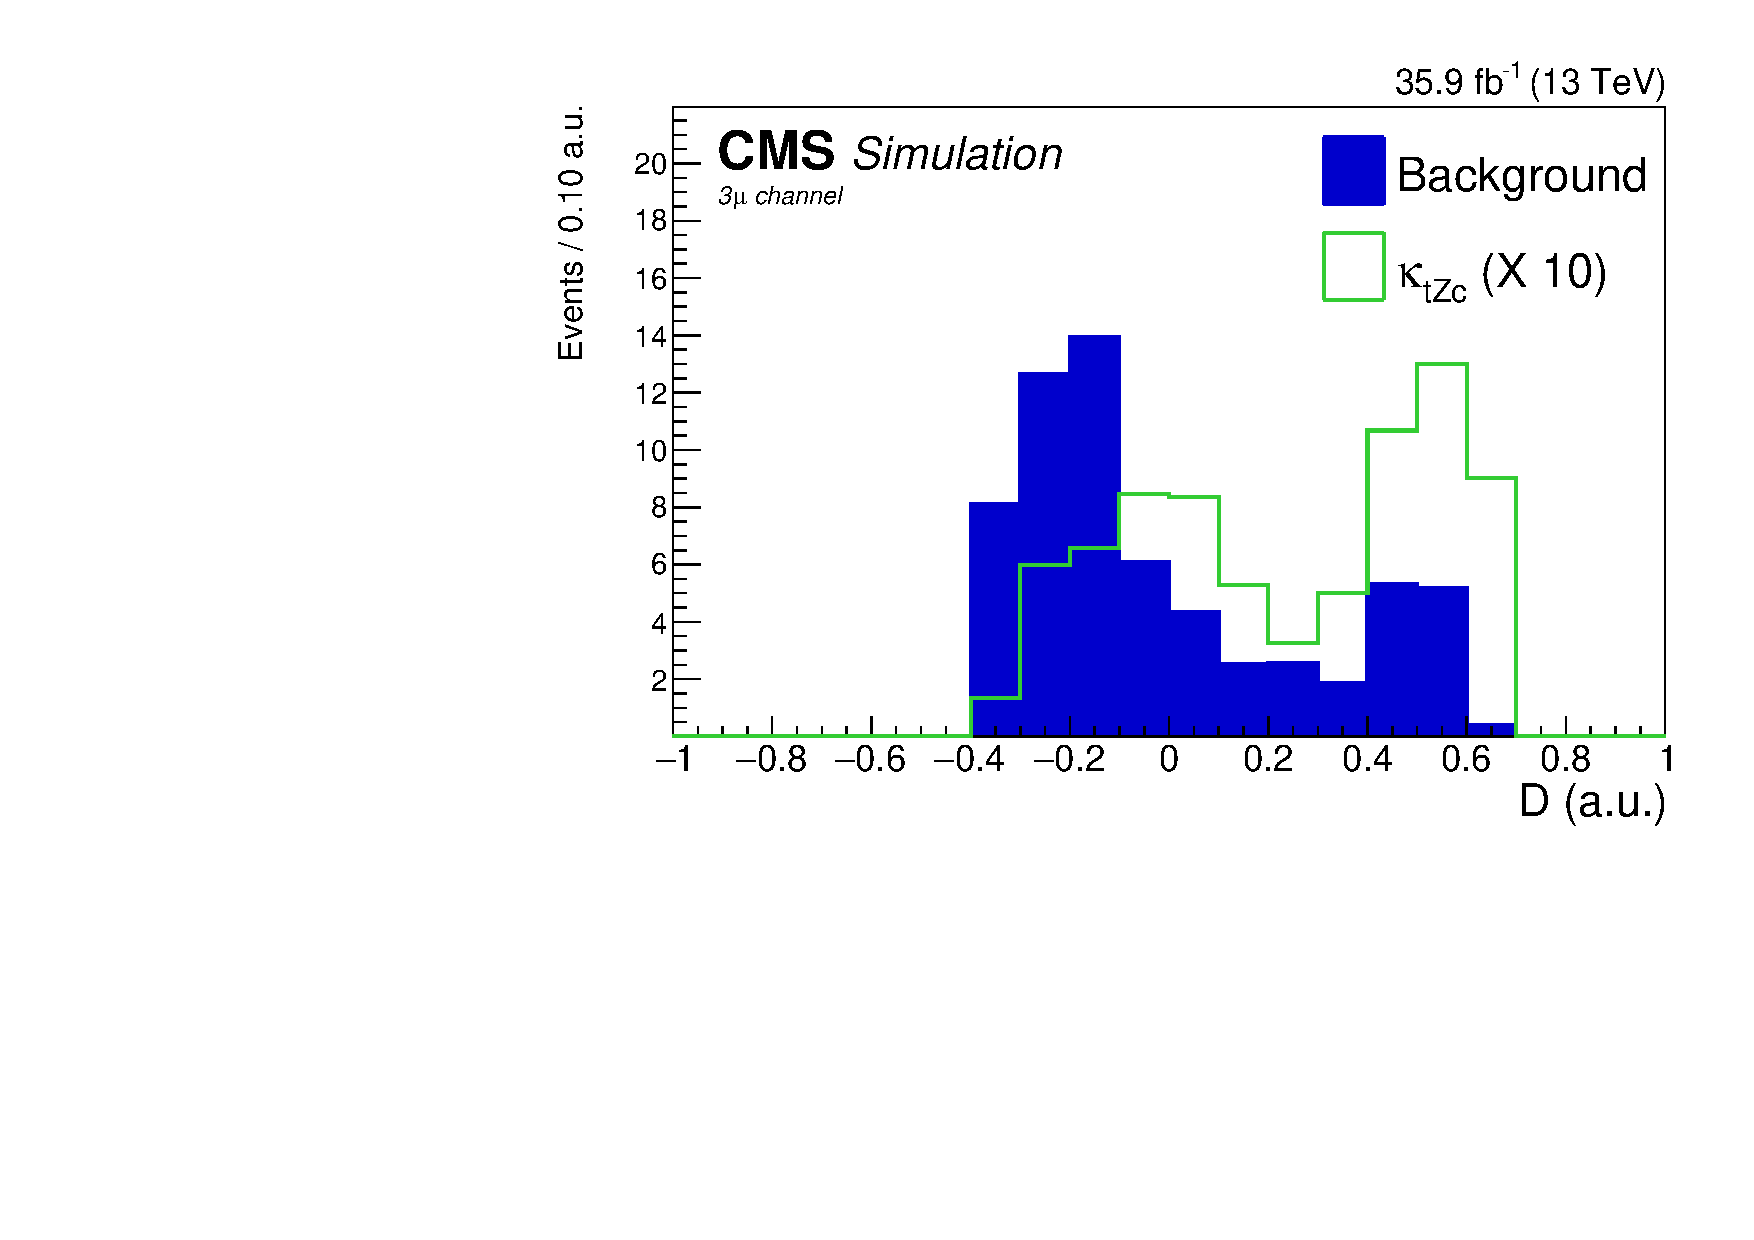
\includegraphics[width=0.47\linewidth]{FiguresAfterUnblinding/BDTunweighted//singletop_Zct_BDT_uuu_Stack}
	\caption{Distributions of the discriminating variable before the fit, \mumumu\  channel. Upper left: \TTSR\ \Zut , upper right: \TTSR\ \Zct ; lower left: \STSR\  \Zut , lower right: \STSR\  \Zct .}
	\label{fig:bdtuuustack}
\end{figure}


\begin{figure}[ht]
	\centering
	% % 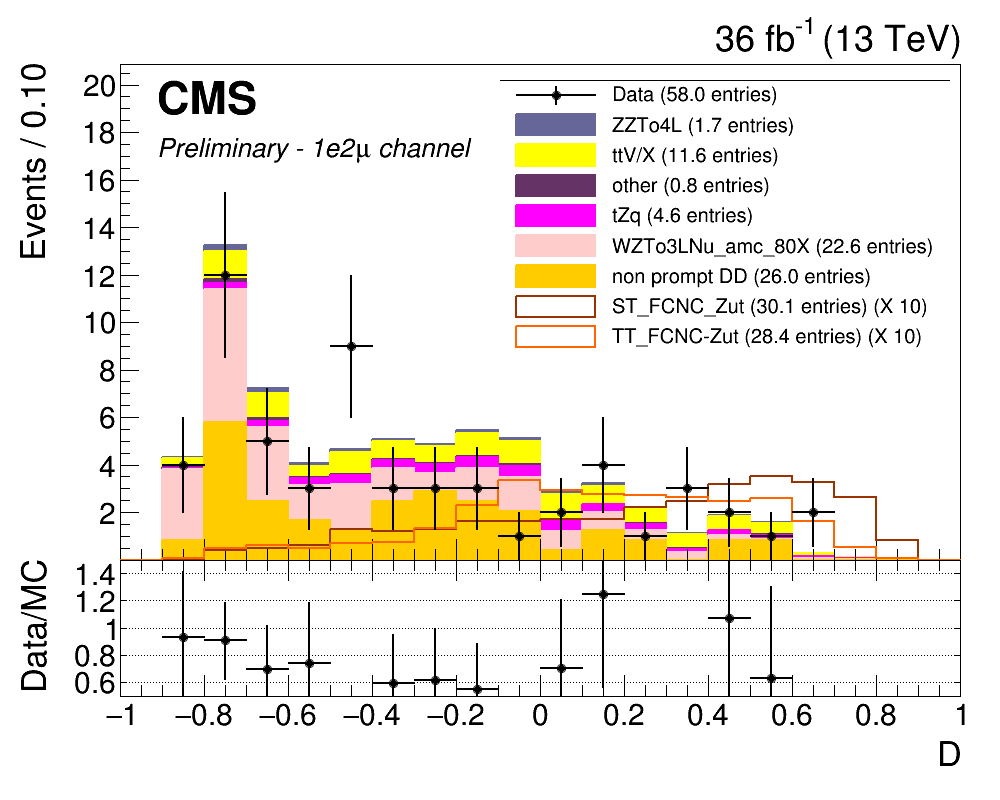
\includegraphics[width=0.47\linewidth]{FiguresAfterUnblinding/BDTunweighted//toppair_Zut_BDT_uue_Stack}
	% % 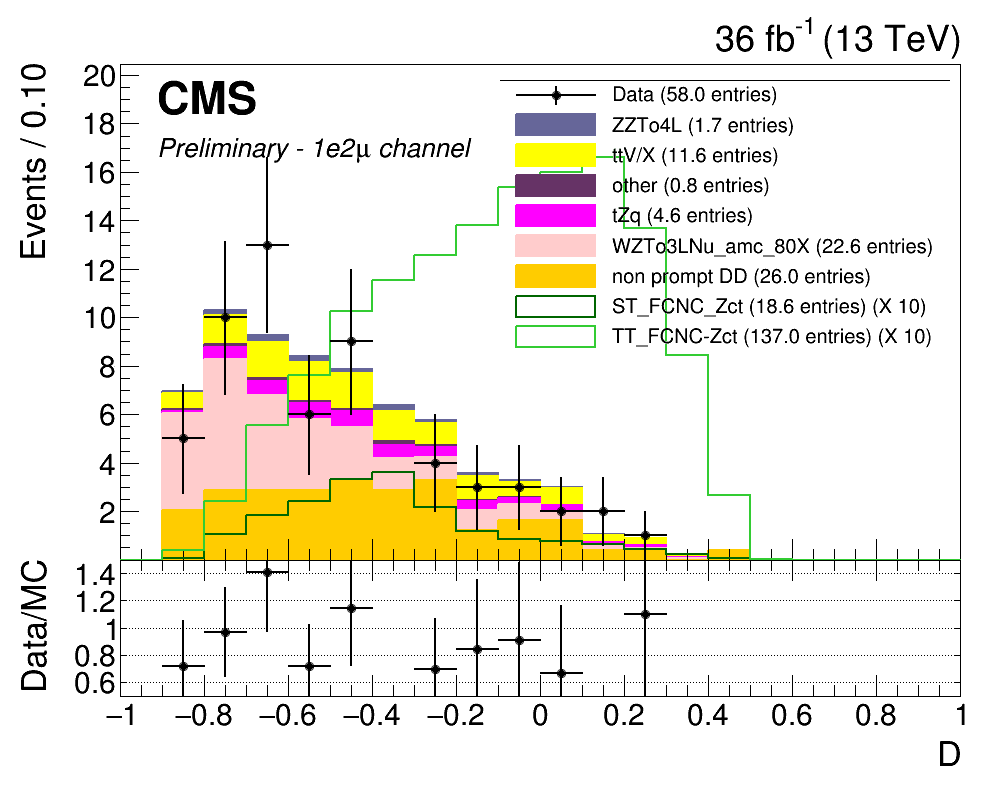
\includegraphics[width=0.47\linewidth]{FiguresAfterUnblinding/BDTunweighted//toppair_Zct_BDT_uue_Stack}
	% % 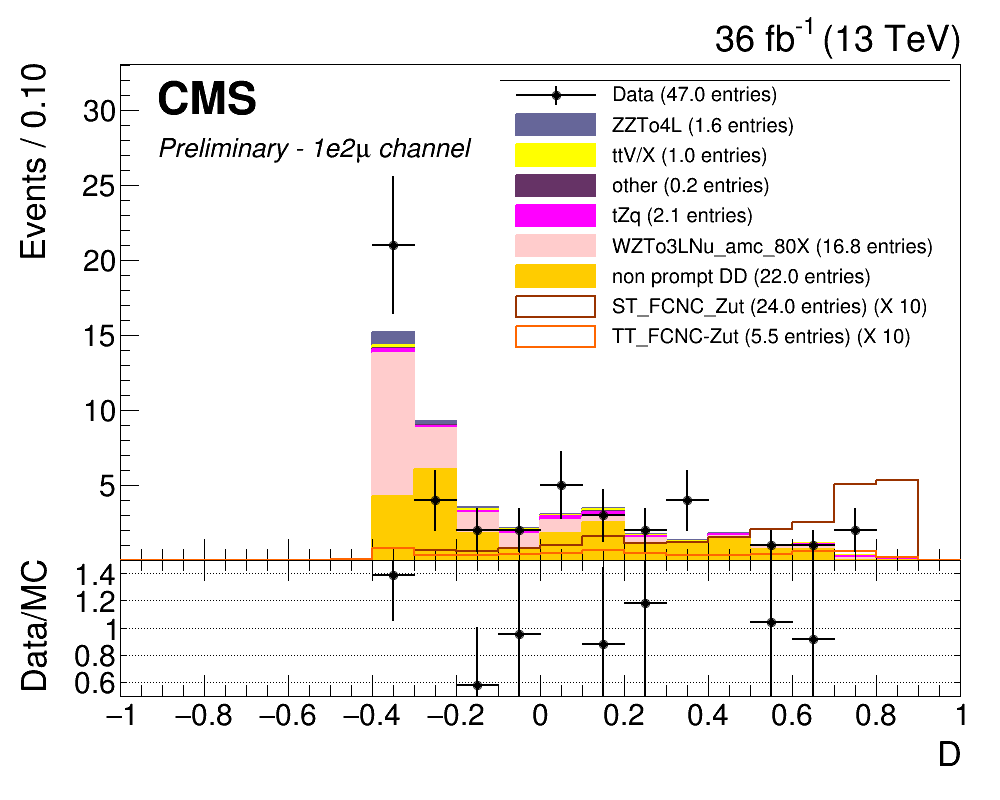
\includegraphics[width=0.47\linewidth]{FiguresAfterUnblinding/BDTunweighted//singletop_Zut_BDT_uue_Stack}
	% % 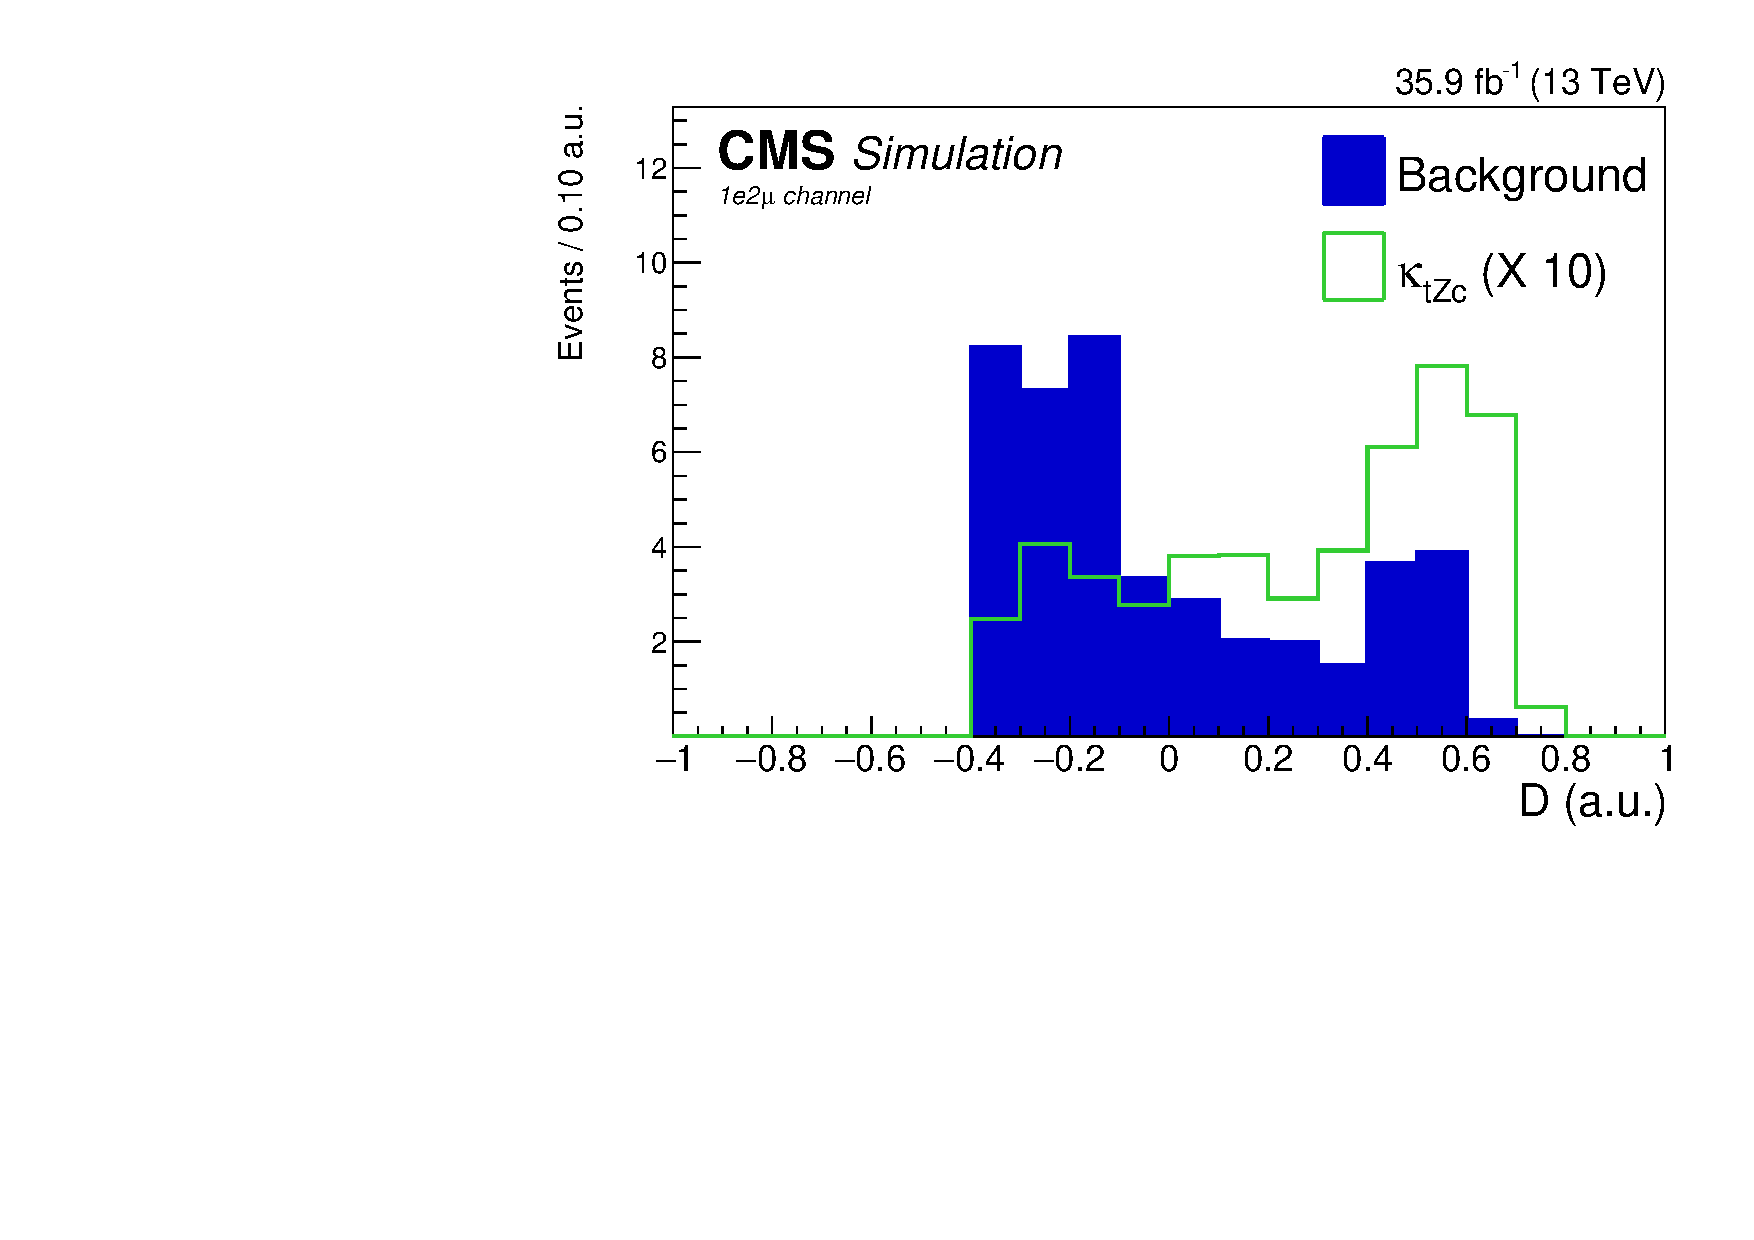
\includegraphics[width=0.47\linewidth]{FiguresAfterUnblinding/BDTunweighted//singletop_Zct_BDT_uue_Stack}
	\caption{Distributions of the discriminating variable before the fit, \emumu\  channel. Upper left: \TTSR\ \Zut , upper right: \TTSR\ \Zct ; lower left: \STSR\  \Zut , lower right: \STSR\  \Zct .}
	\label{fig:bdtuuestack}
\end{figure}

\begin{figure}[ht]
	\centering
	% % 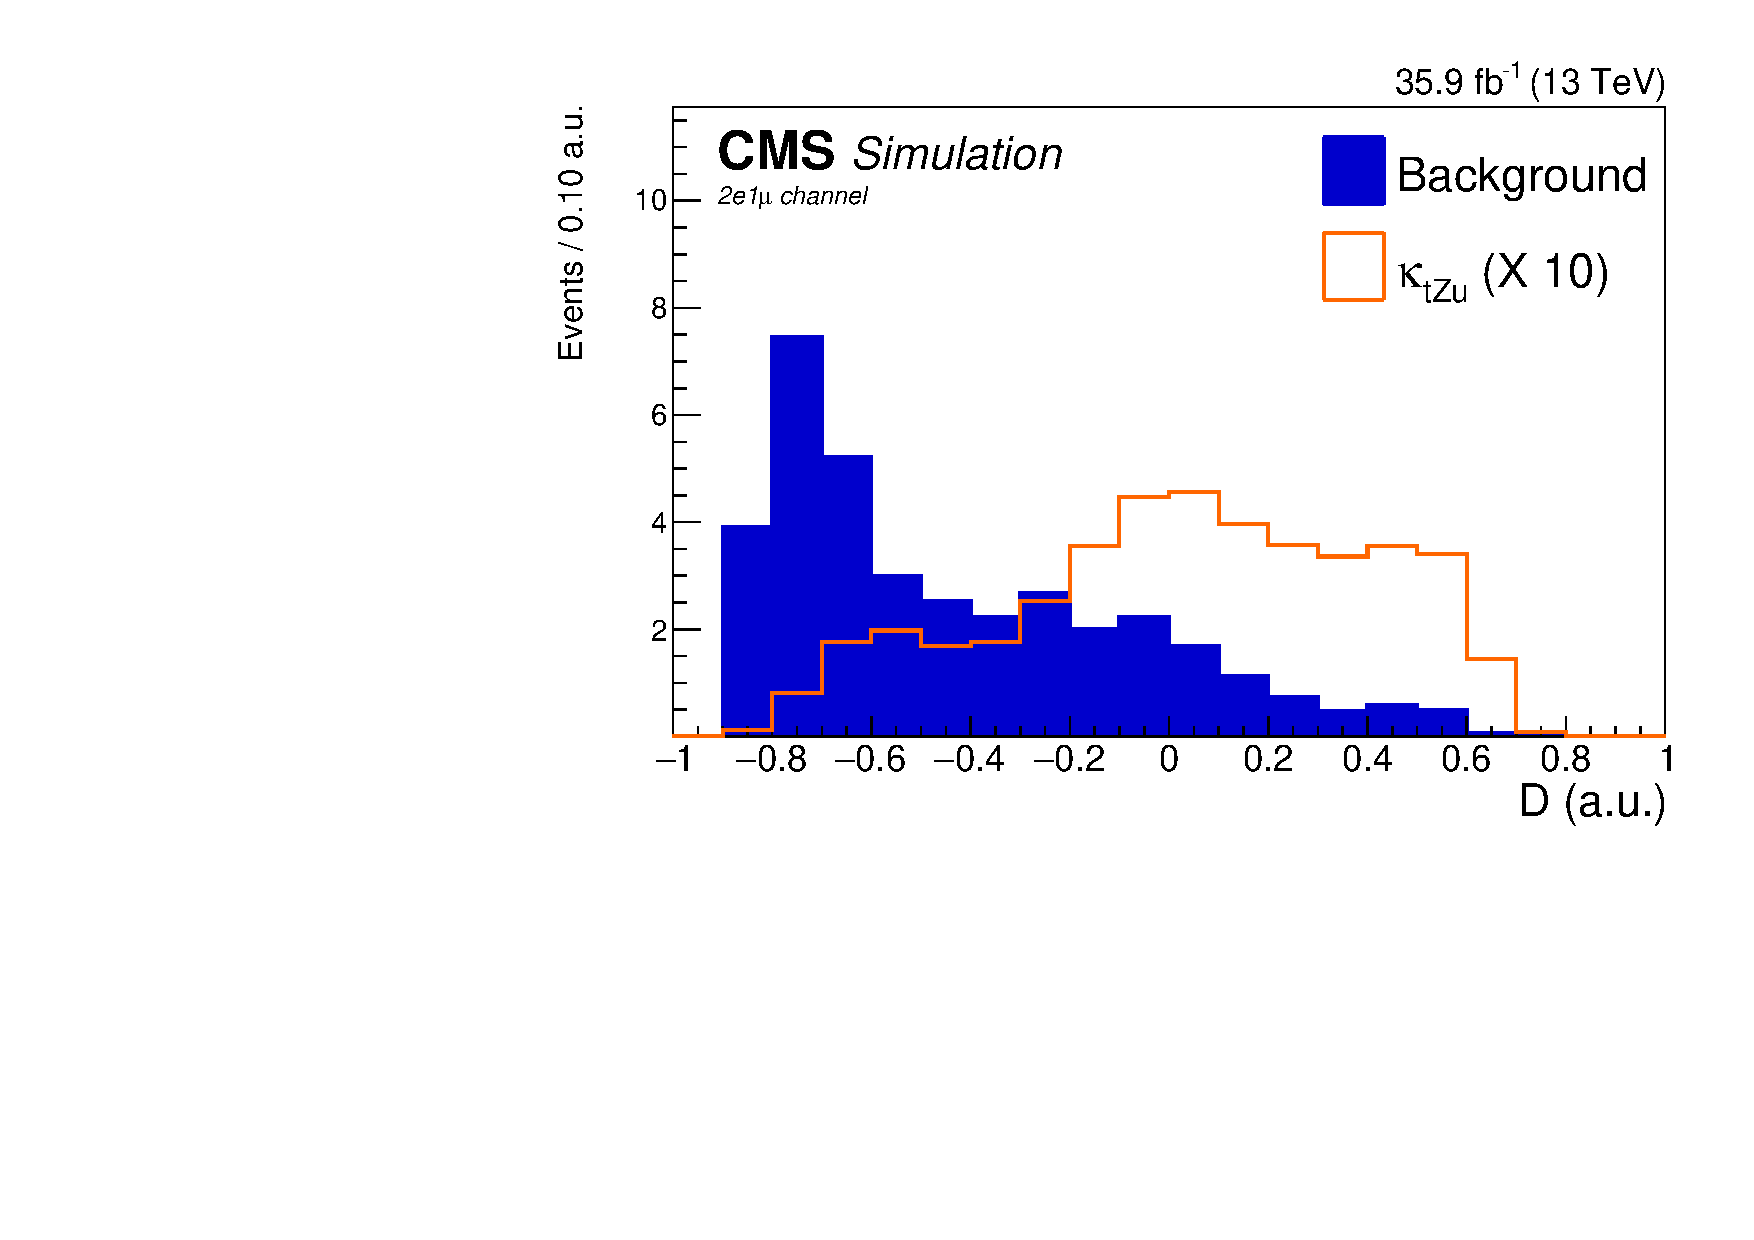
\includegraphics[width=0.47\linewidth]{FiguresAfterUnblinding/BDTunweighted//toppair_Zut_BDT_eeu_Stack}
	% % 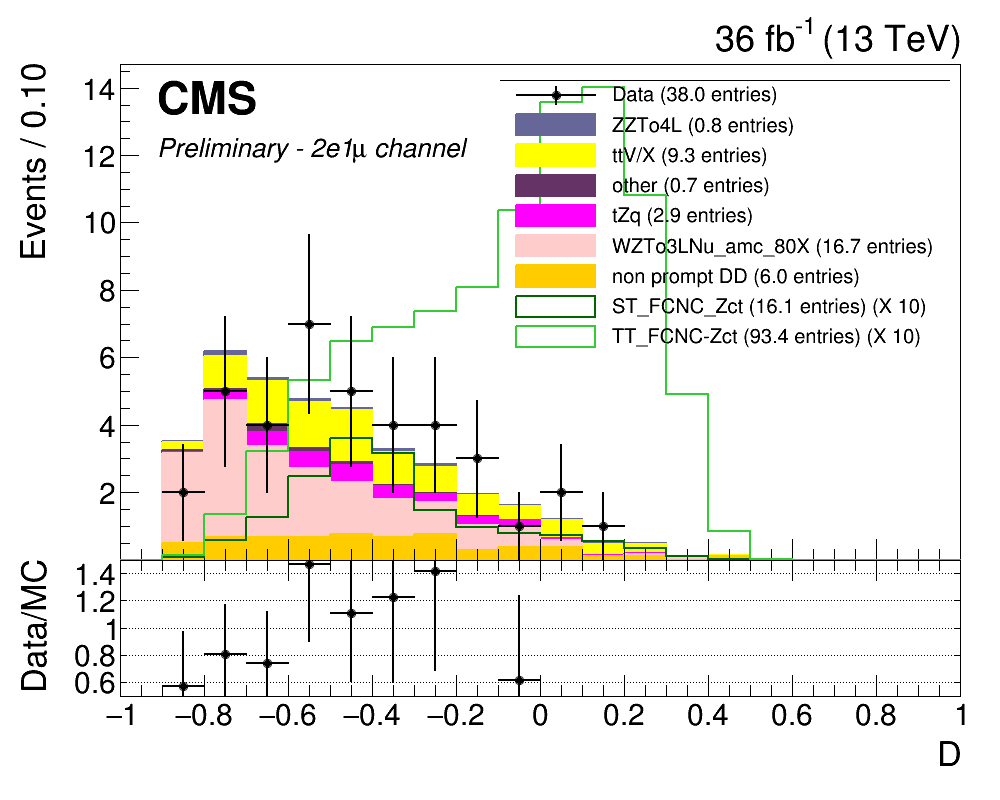
\includegraphics[width=0.47\linewidth]{FiguresAfterUnblinding/BDTunweighted//toppair_Zct_BDT_eeu_Stack}
	% % 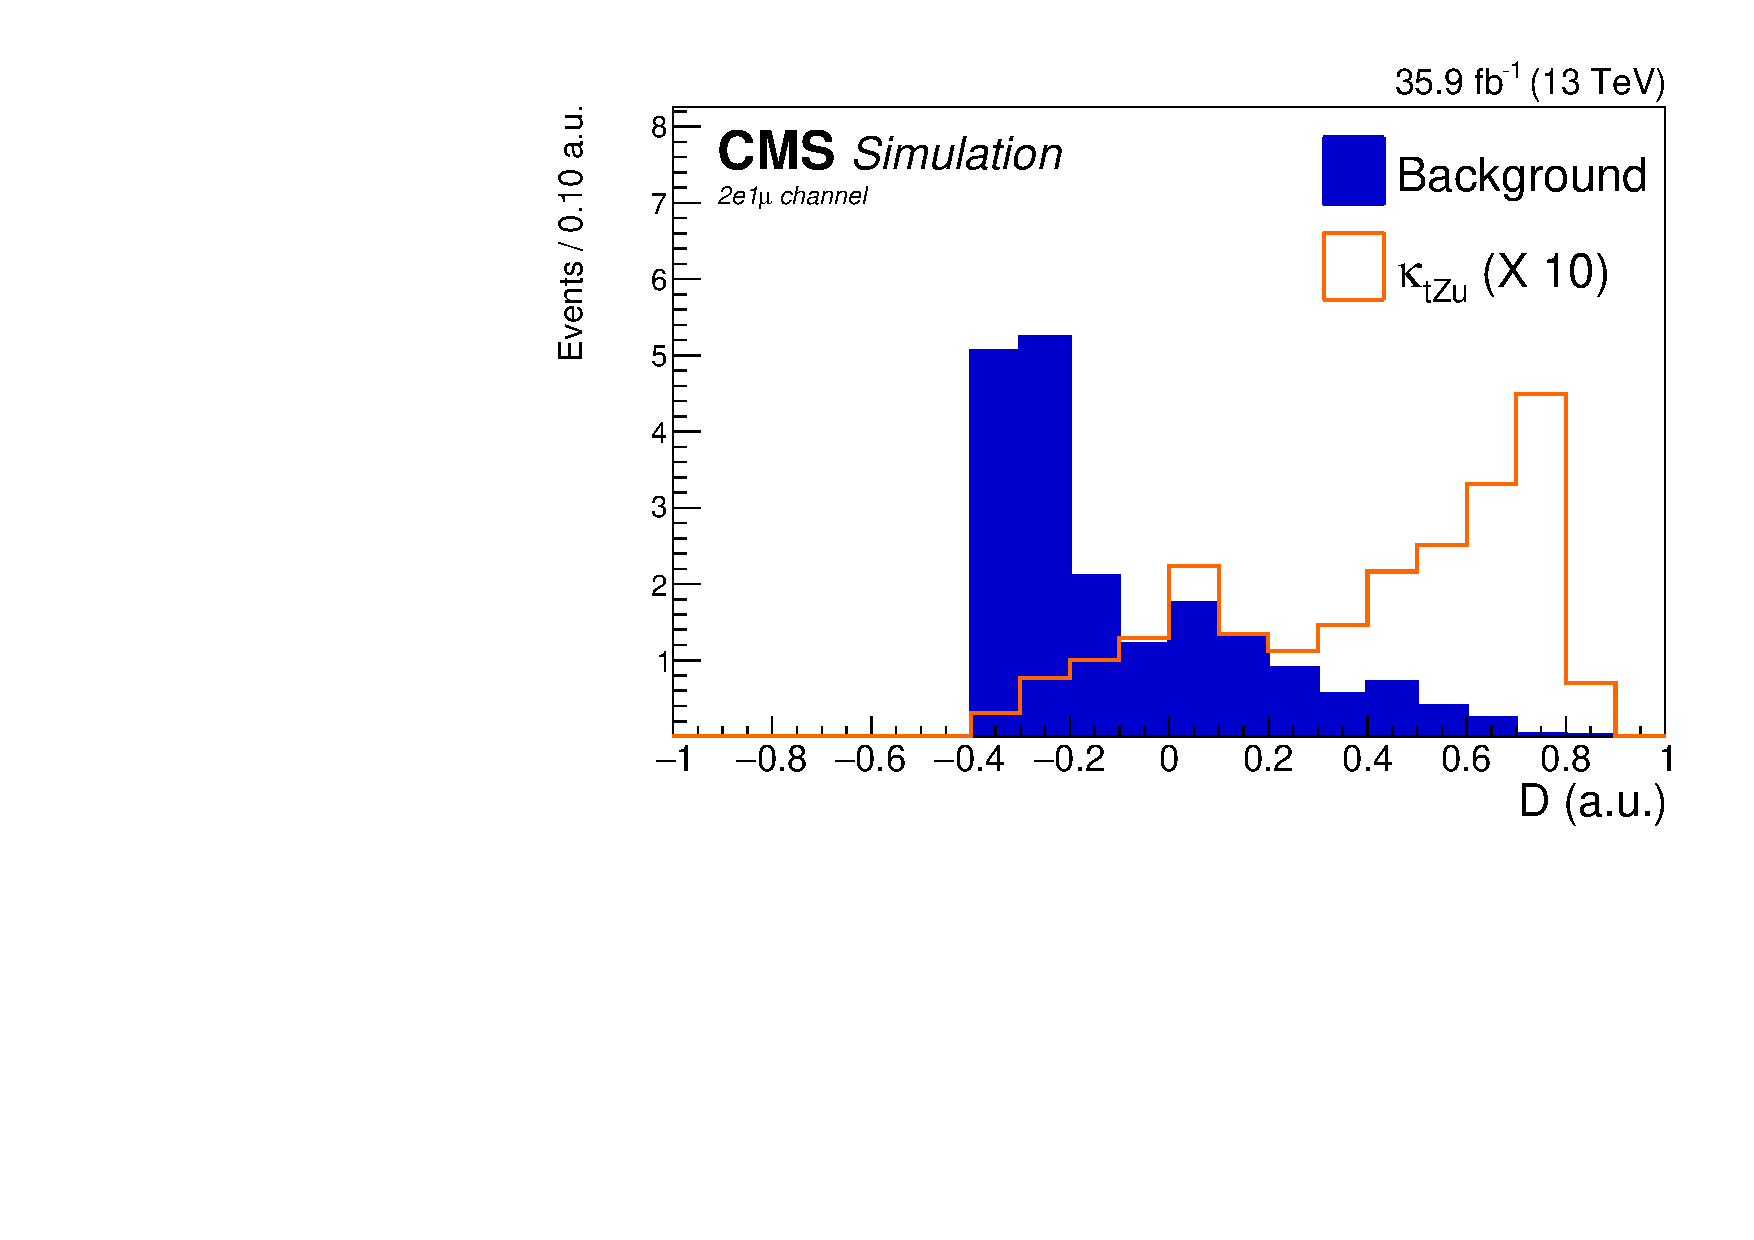
\includegraphics[width=0.47\linewidth]{FiguresAfterUnblinding/BDTunweighted//singletop_Zut_BDT_eeu_Stack}
	% % 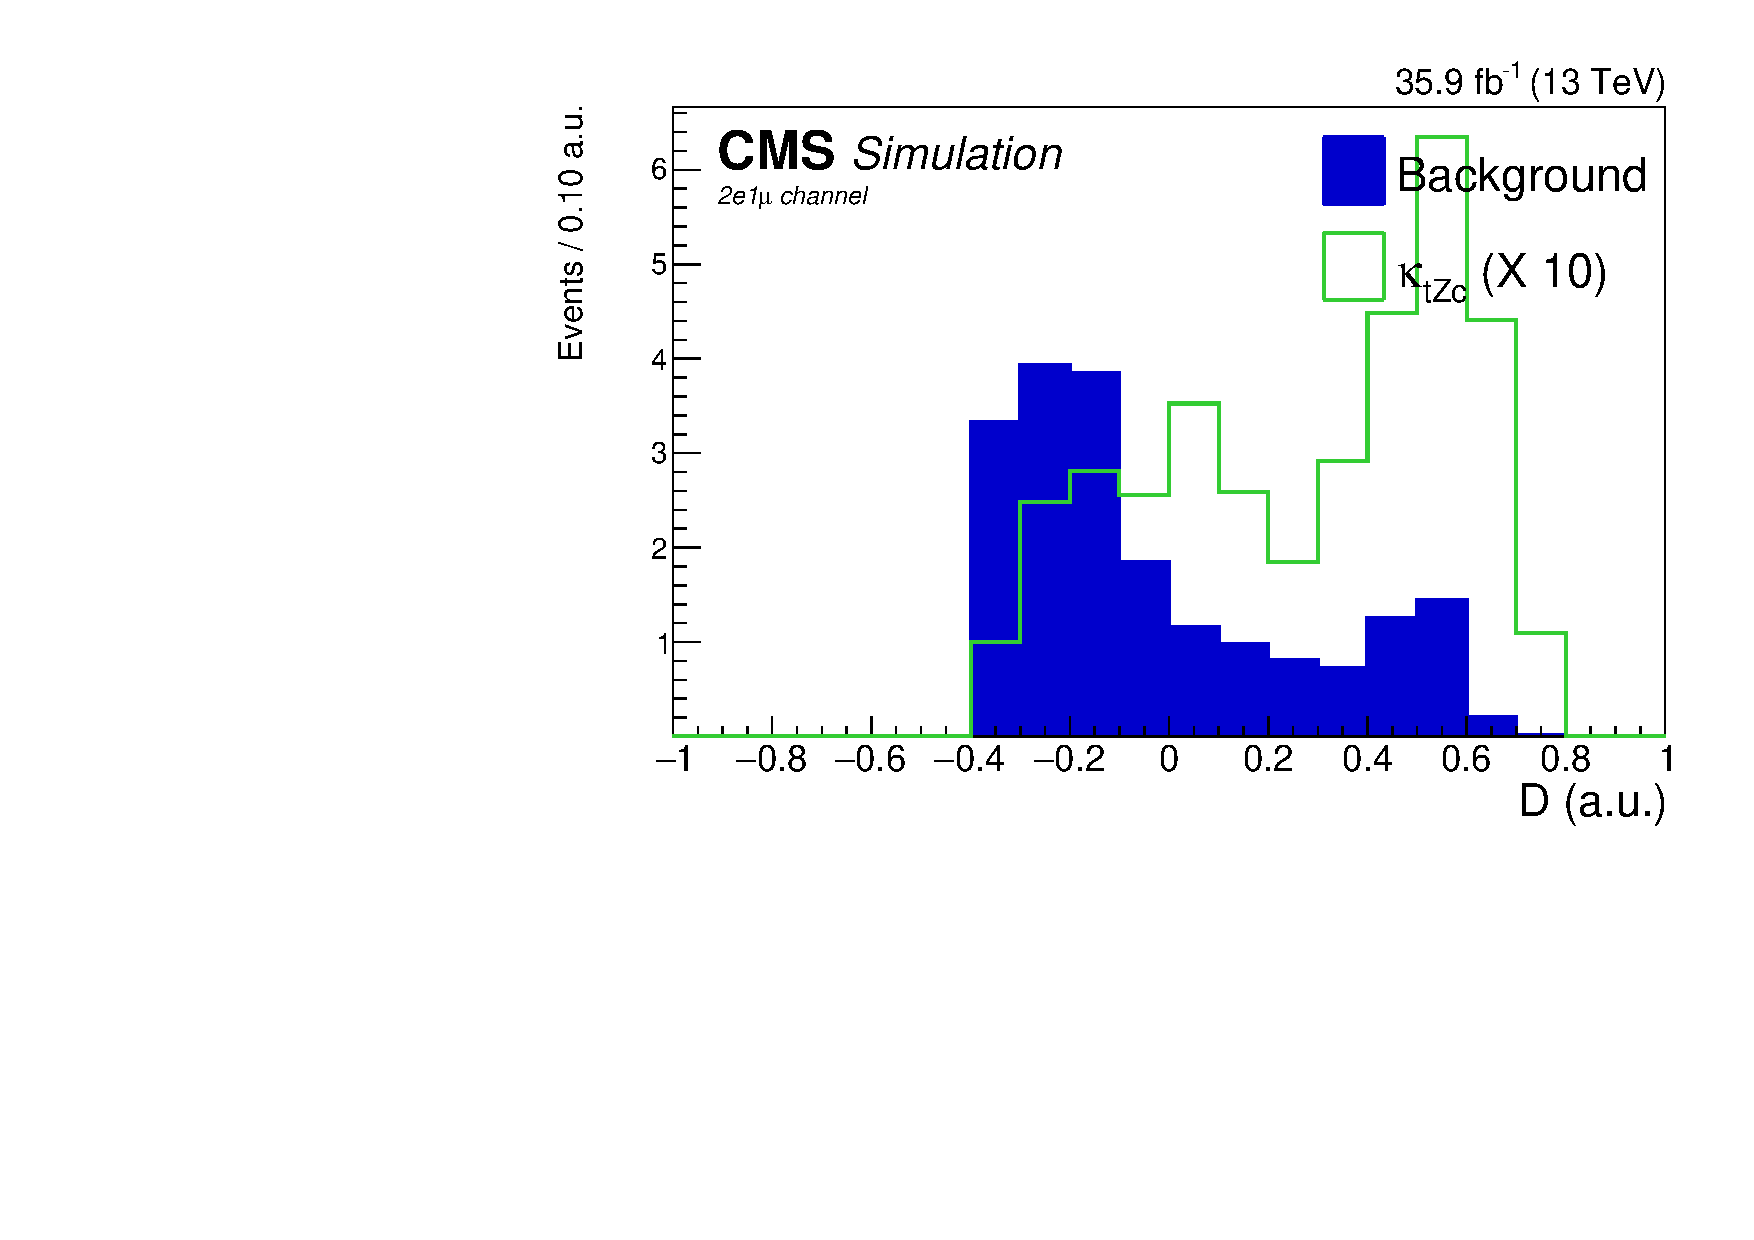
\includegraphics[width=0.47\linewidth]{FiguresAfterUnblinding/BDTunweighted//singletop_Zct_BDT_eeu_Stack}
	\caption{Distributions of the discriminating variable before the fit, \eemu\  channel. Upper left: \TTSR\ \Zut , upper right: \TTSR\ \Zct ; lower left: \STSR\  \Zut , lower right: \STSR\  \Zct .}
	\label{fig:bdteeustack}
\end{figure}



\begin{figure}[ht]
	\centering
	% % 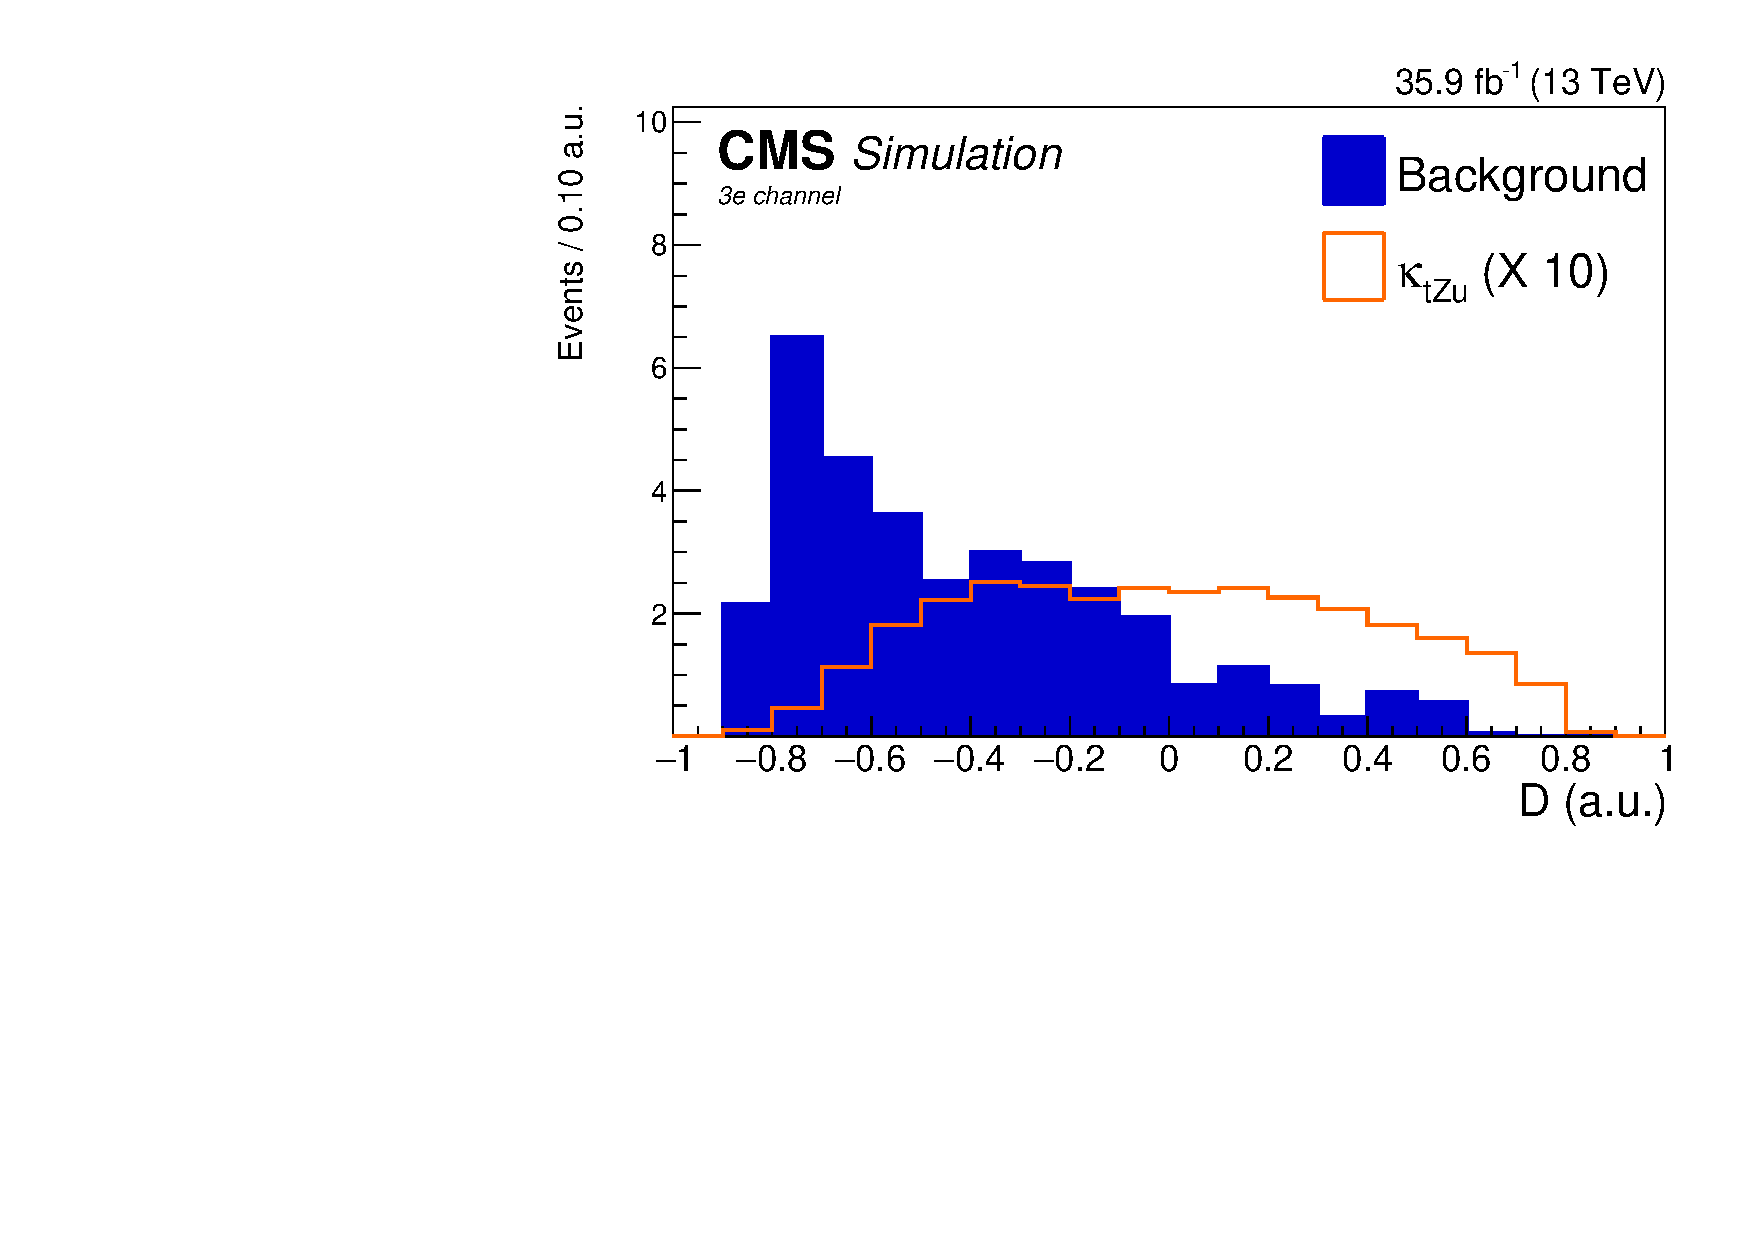
\includegraphics[width=0.47\linewidth]{FiguresAfterUnblinding/BDTunweighted//toppair_Zut_BDT_eee_Stack}
	% % 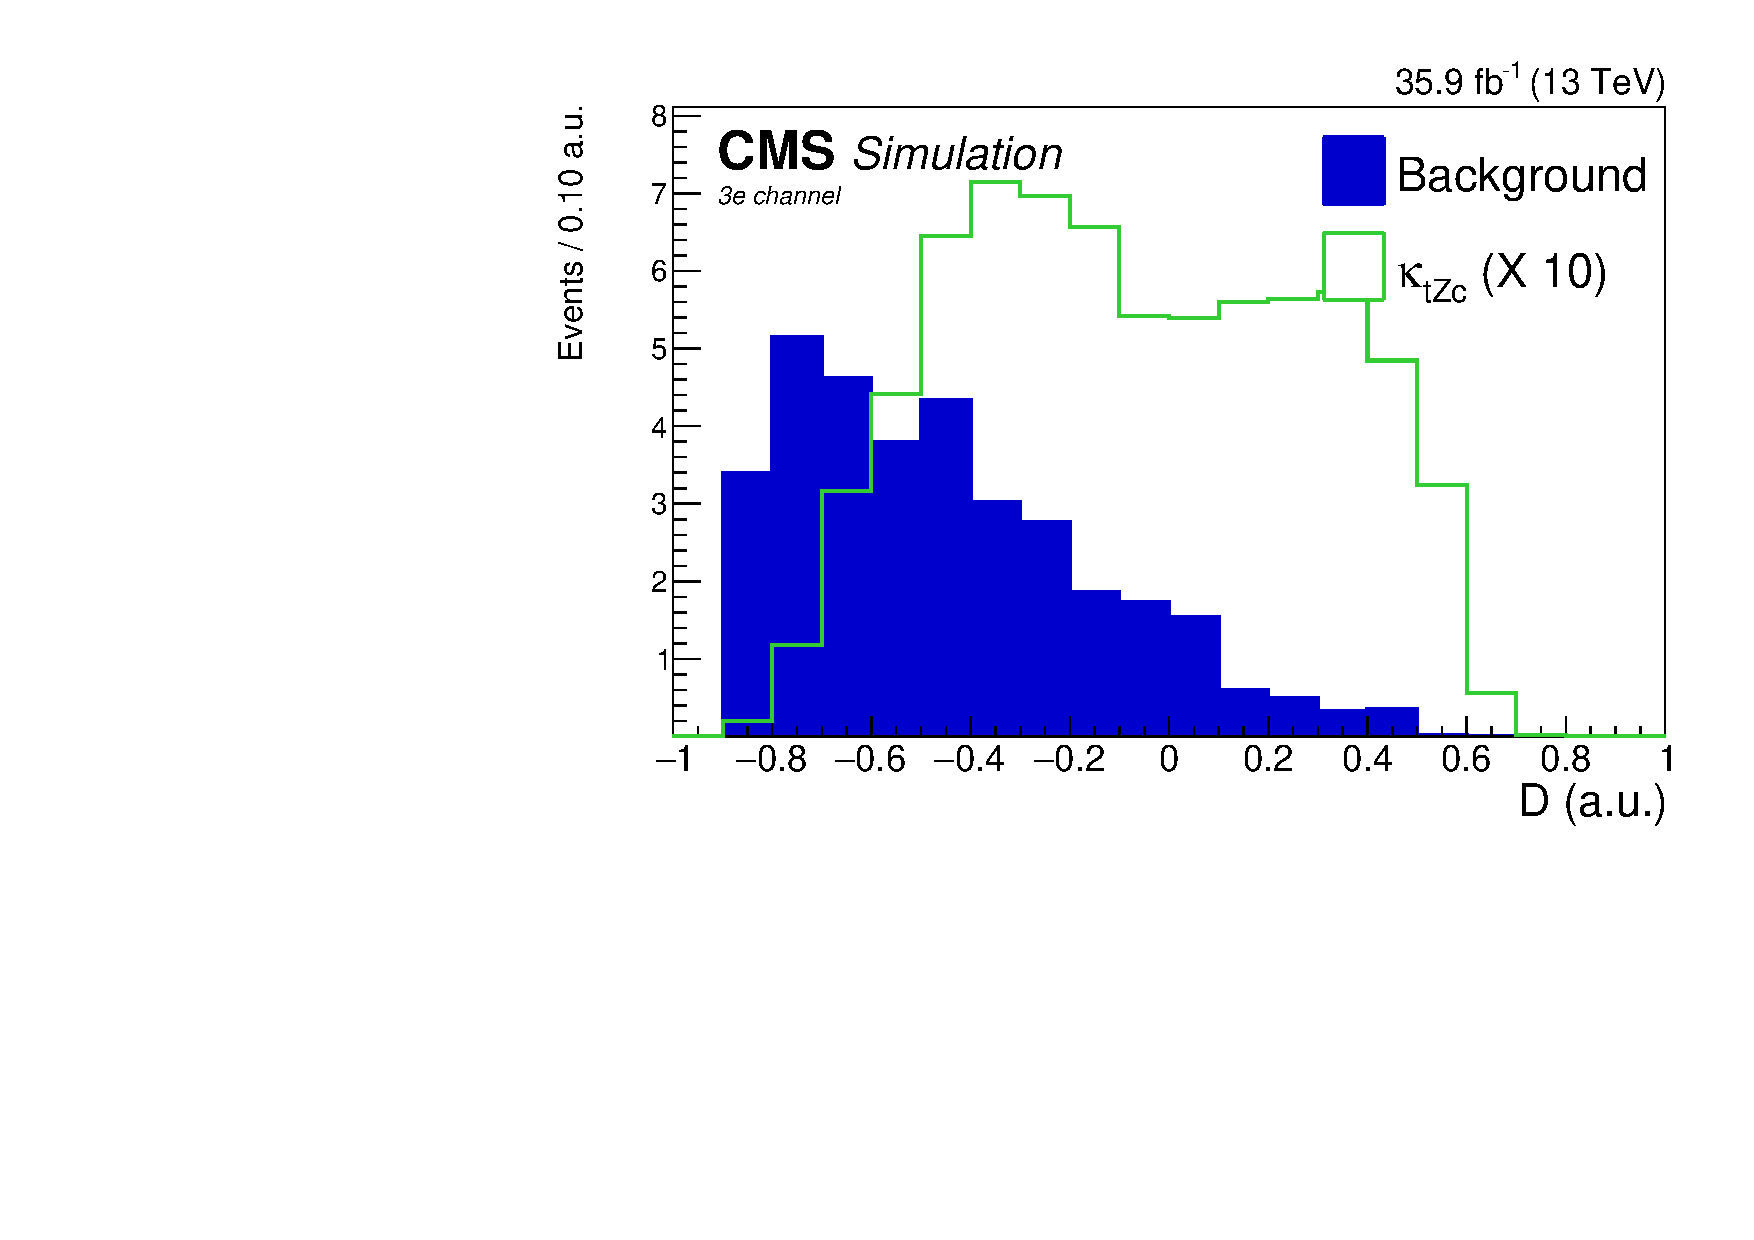
\includegraphics[width=0.47\linewidth]{FiguresAfterUnblinding/BDTunweighted//toppair_Zct_BDT_eee_Stack}
	% % 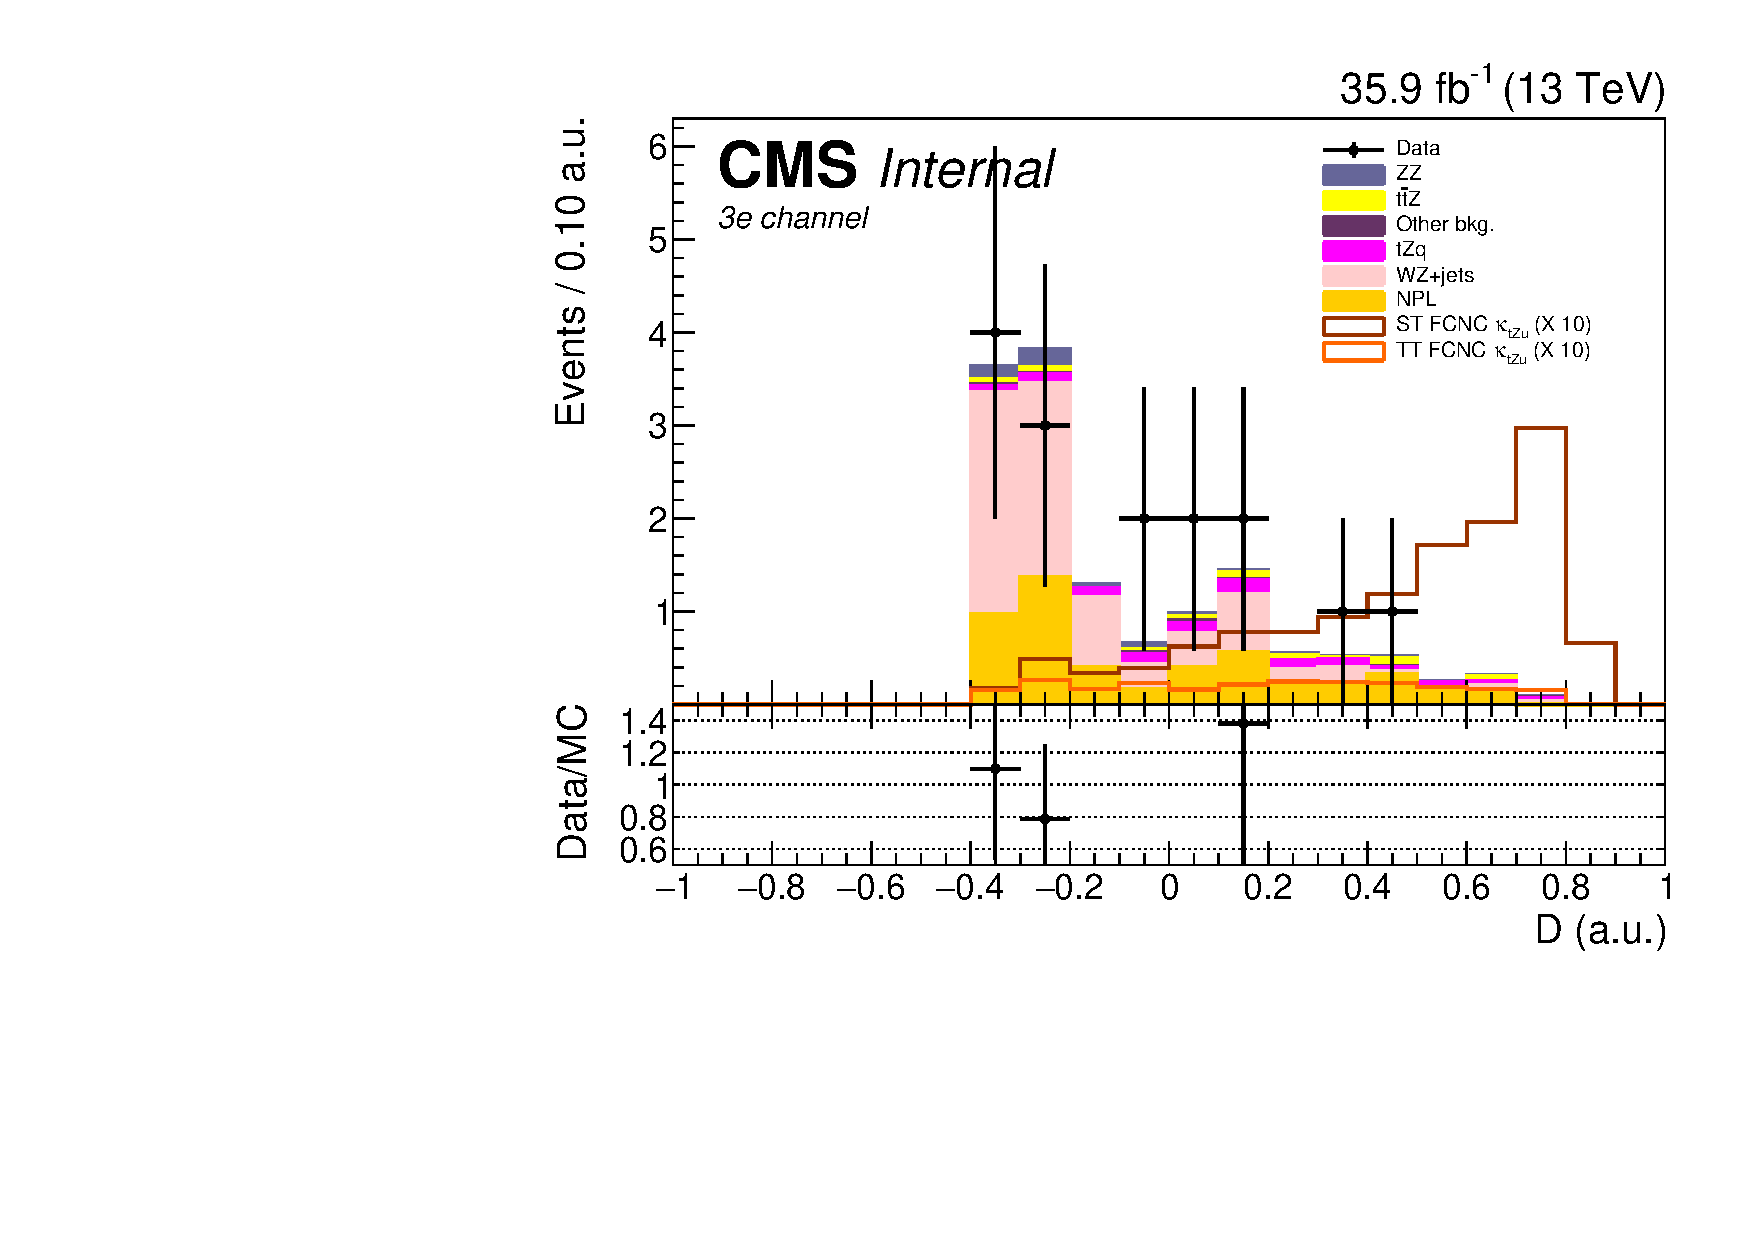
\includegraphics[width=0.47\linewidth]{FiguresAfterUnblinding/BDTunweighted//singletop_Zut_BDT_eee_Stack}
	% % 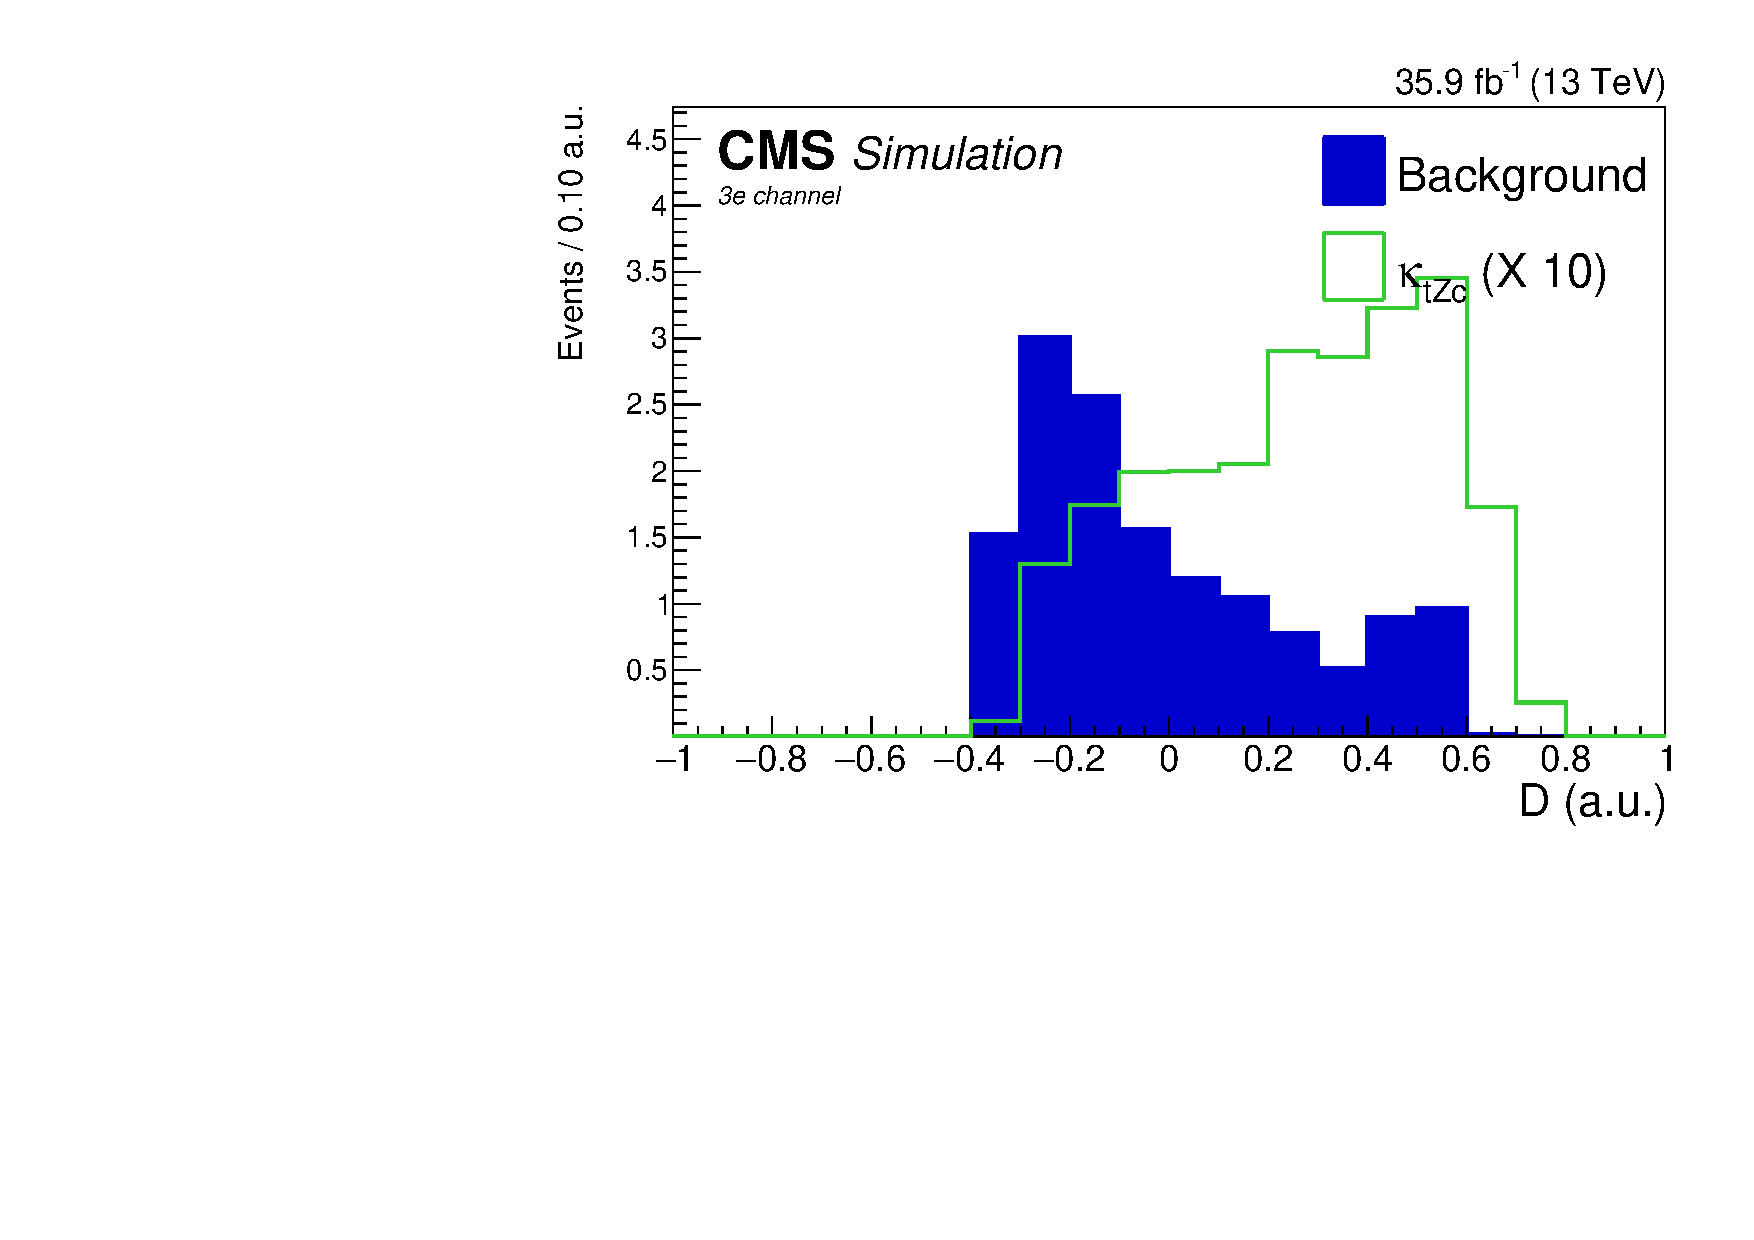
\includegraphics[width=0.47\linewidth]{FiguresAfterUnblinding/BDTunweighted//singletop_Zct_BDT_eee_Stack}
	\caption{Distributions of the discriminating variable before the fit, \eee\  channel. Upper left: \TTSR\ \Zut , upper right: \TTSR\ \Zct ; lower left: \STSR\  \Zut , lower right: \STSR\  \Zct .}
	\label{fig:bdteeestack}
\end{figure}

\subsection{Transverse mass in \WZCR}
The \WZCR\ is used to estimate the contribution from \WZ+jets and \NPL\ background. In this region, a fit is performed on the transverse mass distribution of the \PW\ boson. The pre-fit templates are given in \fig{fig:mtwallstack}. 

\begin{figure}[ht]
	\centering
	% % 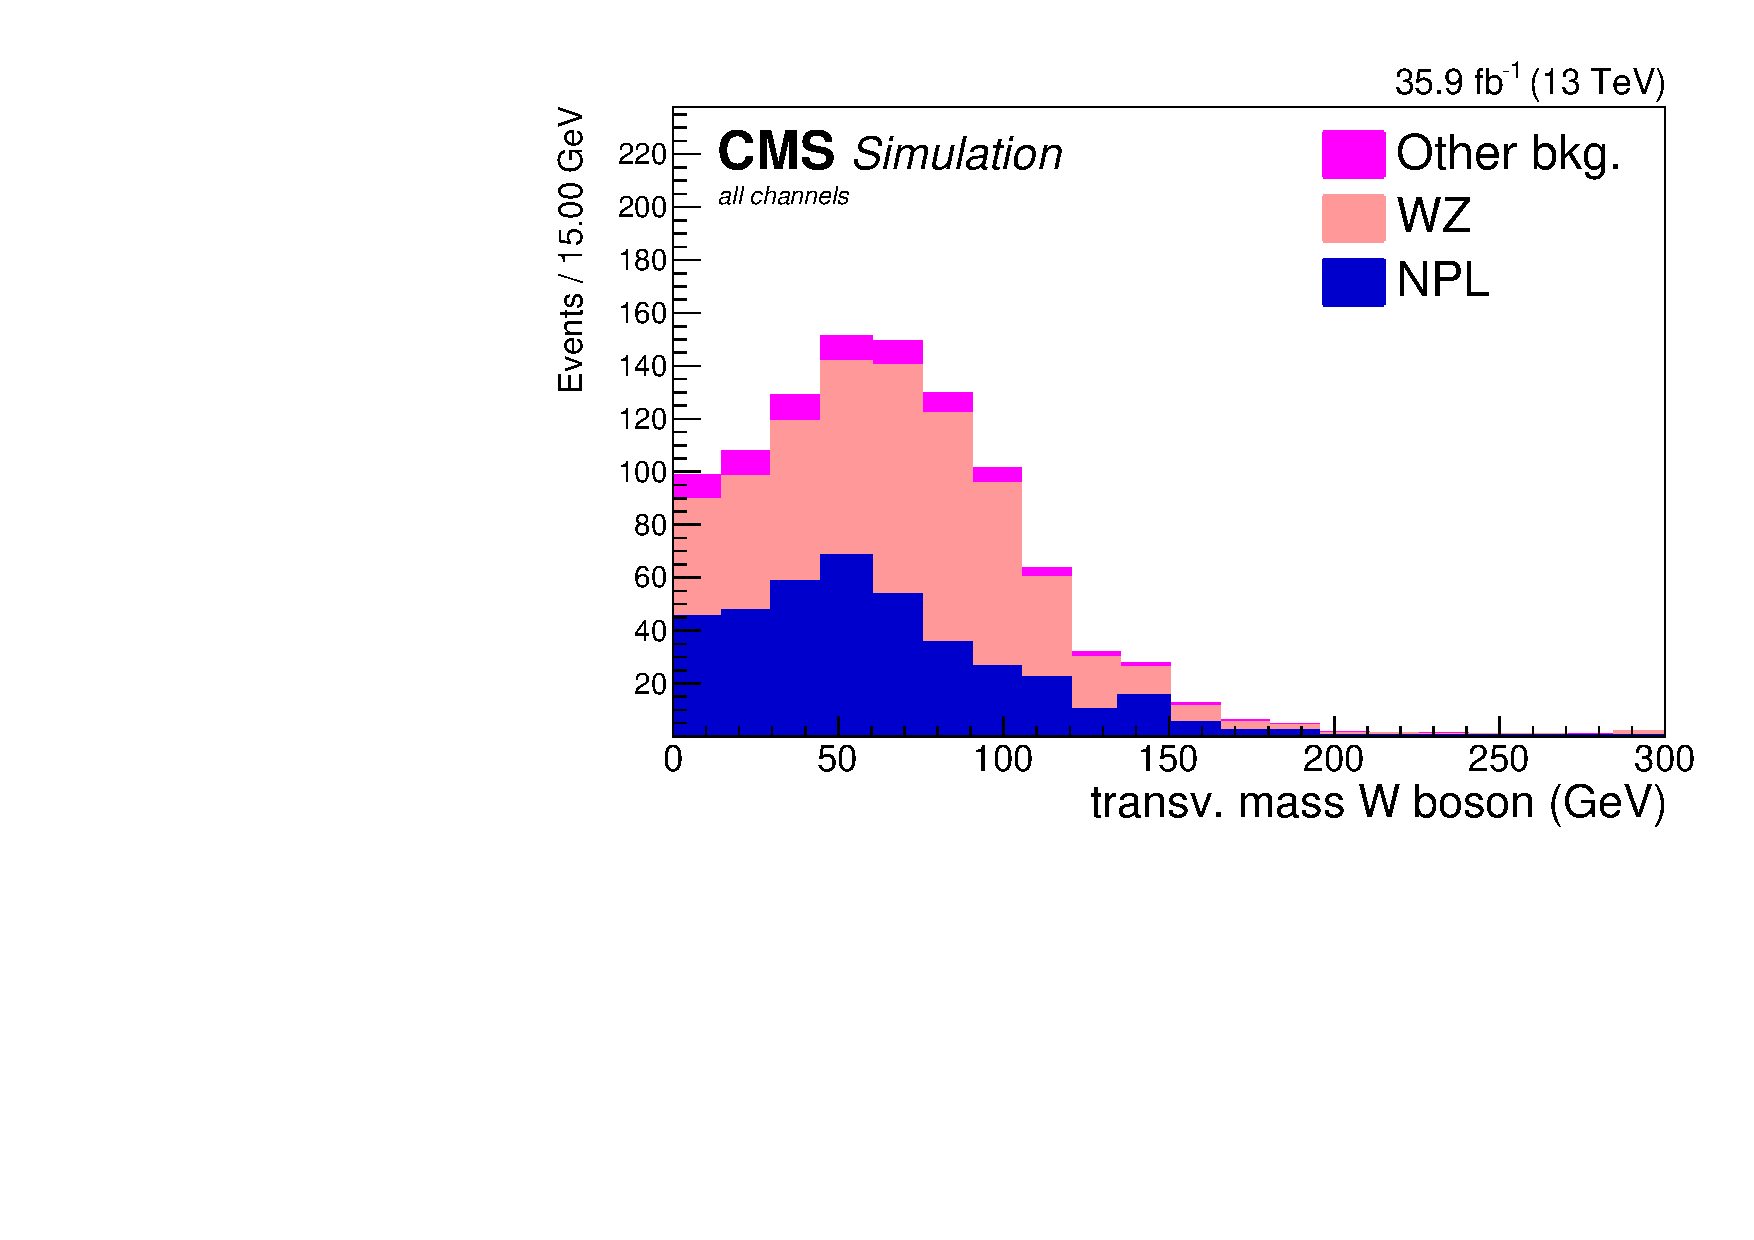
\includegraphics[width=0.47\linewidth]{FiguresAfterUnblinding/MSPlotMTW/MTW_all_Stack}
	% % 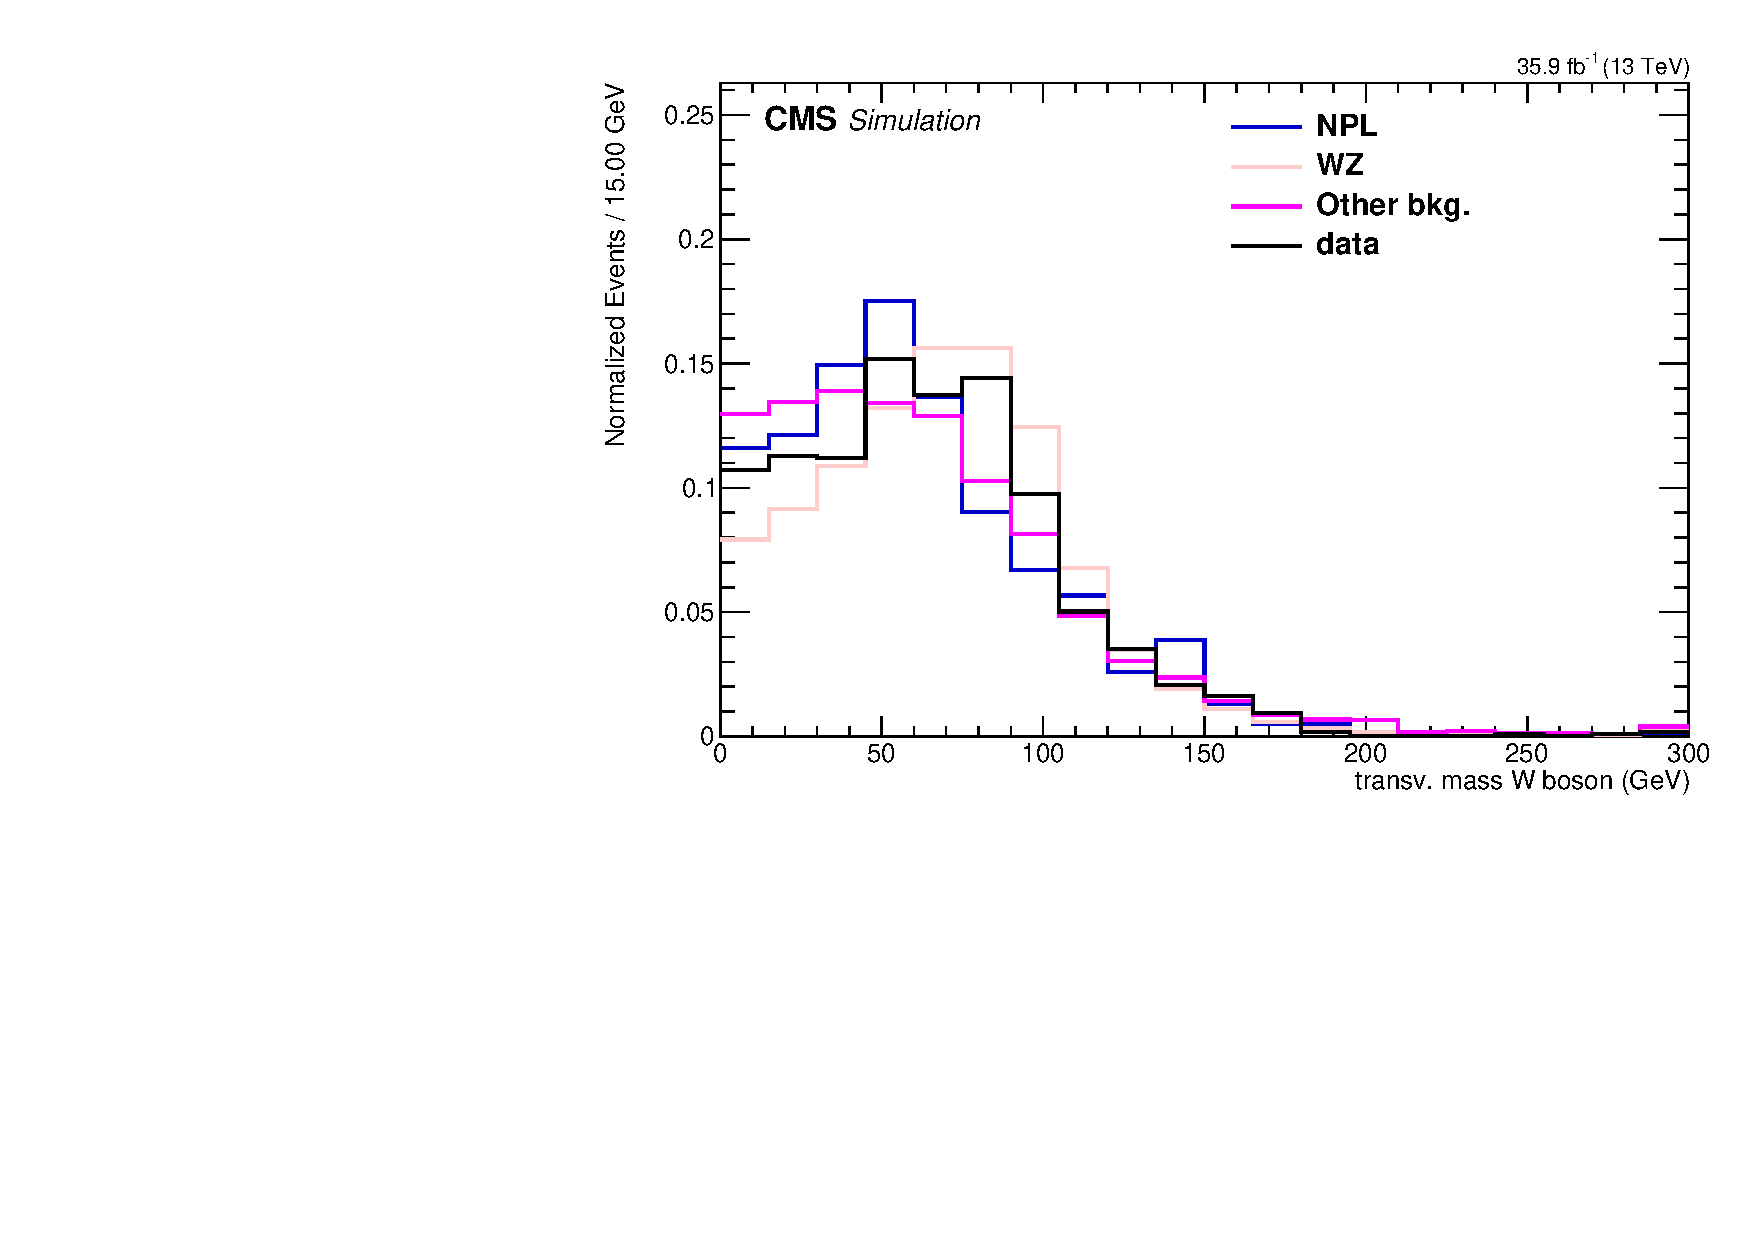
\includegraphics[width=0.37\linewidth]{FiguresAfterUnblinding/MSPlotMTW/MTW_all_Normalized}
	\caption{The transverse mass of the W boson in the \WZCR, before the fit. All different leptonic channels together. Left: scaled to the data, right: normalized.}
	\label{fig:mtwallstack}
\end{figure}

\section{Systematic uncertainties}
The systematic uncertainties entering the analysis are coming from different sources. The experimental uncertainties arise from the reconstruction of the objects and are discussed in \Sec{{sec:PhysicsObject}}. These influence the number of events passing the selection, so-called normalisation uncertainties, or the relative occupancies of the distributions, so-called shape
 uncertainties. The normalisation uncertainties coming from reconstruction include the uncertainty of 2.5\% on the measured integrated luminosity and the efficiency of the trigger logic used for the analysis which has a 1\% (5\%) uncertainty on the 
 \mumumu\ and \emumu (\eemu\ and \eee) channels. The  pileup distribution is calculated via the minimum bias cross section which has a 4.6\% uncertainty. This uncertainty results in a systematic shift in the pileup distribution and its shape effect is estimated by recalculating the pileup distribution for each variation of the minimum bias cross section. The effect of the systematic upwards and downwards shift on the pileup distribution is demonstrated in \Sec{pileupsys}. The shape uncertainties also include the uncertainties coming from the applied lepton scale factors. Their systematic uncertainty originates from three sources: identification, isolation and tracking. The effect of systematic upwards or downwards shift on shapes is demonstrated
 in \Sec{sec:electronsys} and \Sec{sec:muonsys}. The uncertainties arising from jet energy corrections require a recalculation of all jet related kinematic observables and its effect is propagated to the missing transverse energy. The resulting effect of the systematic upwards or downwards shift on shapes is demonstrated in \Sec{sec:JESsys} and \Sec{sec:JERsys}. The reweighting of the CSVv2 discriminant is also a source of uncertainty. There are three sources of uncertainty contributing to the measurement of the b-tag related scale factors: statistical uncertainties, jet energy scale and the purity of the sample. These result in eight uncorrelated contributions for which the effects on the shapes are shown in \Sec{sec:btagsys}. 
 
 Since the \NPL\ sample is artificially made from data by inverting the isolation of the third lepton. Its effect has to be estimated. The shape uncertainty one the \NPL\ processes is obtained by varying the isolation inversion with respect to tight working point to the loose working point for electrons and muons at the same time. This found to have negligible effect. The uncertainty on the normalisation of the overall \NPL\ yield is taken as 50\% in accordance the the \SM\ \tZq\ search\todocite.
 
 The uncertainty on the expected yield of the simulated backgrounds is taken to be 30\% of the yield such that it covers all uncertainties at next to leading order accuracy. Theory uncertainties  originating from the modelling of the main backgrounds are estimated to account for the effect on the shape of the distributions from the choice of parton density funnctions, and renormalization (\muR) and factorization (\muF) scales. The effect of the  renormalization (\muR) and factorization (\muF) scales is estimated by varying each independently and correlated up and down by a factor of two, where the anti-correlated variations are dropped. The envelope of these variations is used as an uncertainty. The uncertainties coming from the parton density functions  used for simulation are estimated using the PDF4LHC recipe~\cite{Ball:2017nwa}, which combines the MMHT14, CT14, and NNPDF3.0 PDF sets~\cite{Ball:2017nwa}. The theory uncertainties are considered for the main backgrounds coming from simulation: \WZ+jets, \ZZ+jets, \ttZ, and \tZq. This is found to have a negligible effect.

 The way the uncertainties are treated as nuisance parameters is summarized in Table \ref{tab:nuis}.

\begin{table}[htbp]
	\centering
	\caption{Uncertainties used in this analysis. The column labelled type represents how the uncertainty is treated for the fit.}
	\begin{tabular}{ccc}
		\toprule
		Source & Systematic input & Type \\ 
		\midrule 
		nonprompt muon norm. & 50\% & normalisation \\ 
		 
		nonprompt electron norm. & 50\% & normalisation \\ 
		 
		background \ttZ\ norm. & 30\% & normalisation \\ 
		 
		background \WZ\ norm. & 30\% & normalisation \\ 
		 
		background \tZq\ norm. & 30\% & normalisation \\ 
		 
		background \ZZ\ norm.& 30\% & normalisation \\ 
		 
		background other MC norm. & 30\% & normalisation \\ 
		 
		trigger & 1\% (5\%) & normalisation \\ 
		 
		lepton identification  & $\pm \sigma(p_{T},\eta)$ & shape \\ 
		 
		JES & $\pm \sigma(p_{T},\eta)$ & shape \\ 
		 
		JER & $\pm \sigma(p_{T},\eta)$ &  shape \\ 
		 
		b-tagging & $\pm \sigma(p_{T},\eta)$ & shape \\ 
		 
		pileup\ & $\pm \sigma$ of min. bias cross section &  shape \\ 
		 
		PDF & PDF4LHC recipe &  shape (WZ,tZq, ttZ, ZZ)  \\ 
		 
		luminosity & 2.5\% & normalisation \\ 
		 
		renorm. and fact. scales & varying indep. and corr. &  shape \\ 
		\bottomrule
	\end{tabular} 
	\label{tab:nuis}
\end{table}
\begin{comment}
\subsection{Effect of pile up on the shapes}
\label{sec:pileupsys}
\begin{figure}[h] 
	\centering 
	% 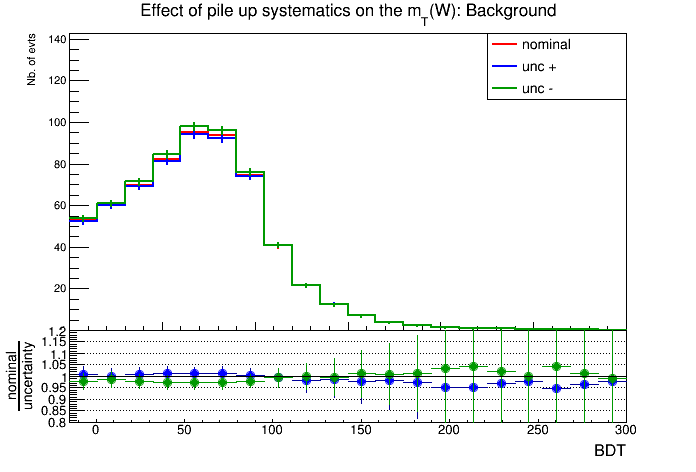
\includegraphics[width=0.48\textwidth]{Figures/boosteddecisiontrees/MTWsys/hist_mWt_puSF_nom_bkg}
	\caption{Distribution of the nominal values and shift due to pile up uncertainties for the transverse mass of the \PW\ boson in the \WZCR. All channel.}
	\label{fig:pileupshiftmtWSTzct}
\end{figure}
\begin{figure}[h] 
	\centering
	% \subfigure[Background]{% \includegraphics[width=0.48\textwidth]{Figures/boosteddecisiontrees/singletopzct/systematics/hist_BDT_puSF_nom_bkg}}
	% \subfigure[Signal]{% \includegraphics[width=0.48\textwidth]{Figures/boosteddecisiontrees/singletopzct/systematics/hist_BDT_puSF_nom_sig}}
	\caption{Distribution of the nominal values and shift due to pile up uncertainties for the BDT discriminant for the \Zct\ vertex in the \STSR. All channel.}
	\label{fig:pileupshiftBDTSTzct}
\end{figure}
\begin{figure}[h] 
	\centering
	% \subfigure[Background]{% \includegraphics[width=0.48\textwidth]{Figures/boosteddecisiontrees/singletopzut/systematics/hist_BDT_puSF_nom_bkg}}
	% \subfigure[Signal]{% \includegraphics[width=0.48\textwidth]{Figures/boosteddecisiontrees/singletopzut/systematics/hist_BDT_puSF_nom_sig}}
	\caption{Distribution of the nominal values and shift due to pile up uncertainties for the BDT discriminant for the \Zut\ vertex in the \STSR. All channel.}
	\label{fig:pileupshiftBDTSTzut}
\end{figure}
\begin{figure}[h] 
	\centering
	% \subfigure[Background]{% \includegraphics[width=0.48\textwidth]{Figures/boosteddecisiontrees/toppairzct/systematics/hist_BDT_puSF_nom_bkg}}
	% \subfigure[Signal]{% \includegraphics[width=0.48\textwidth]{Figures/boosteddecisiontrees/toppairzct/systematics/hist_BDT_puSF_nom_sig}}
	\caption{Distribution of the nominal values and shift due to pile up uncertainties for the BDT discriminant for the \Zct\ vertex in the \TTSR. All channel.}
	\label{fig:pileupshiftBDTTTzct}
\end{figure}
\begin{figure}[h] 
	\centering
	% \subfigure[Background]{% \includegraphics[width=0.48\textwidth]{Figures/boosteddecisiontrees/toppairzut/systematics/hist_BDT_puSF_nom_bkg}}
	% \subfigure[Signal]{% \includegraphics[width=0.48\textwidth]{Figures/boosteddecisiontrees/toppairzut/systematics/hist_BDT_puSF_nom_sig}}
	\caption{Distribution of the nominal values and shift due to pile up uncertainties for the BDT discriminant for the \Zut\ vertex in the \TTSR. All channel.}
	\label{fig:pileupshiftBDTTTzut}
\end{figure}


\subsection{Effect of electron scale factors on the shapes}
\label{sec:electronsys}

\begin{figure}[h] 
	\centering
	% 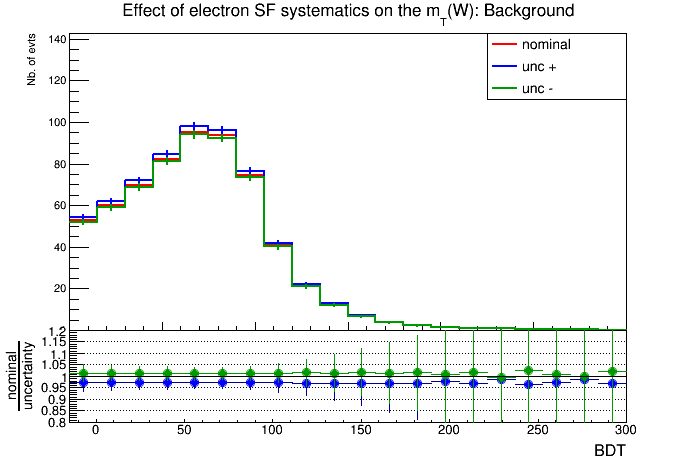
\includegraphics[width=0.48\textwidth]{Figures/boosteddecisiontrees/MTWsys/hist_mWt_electronSF_nom_bkg}
	\caption{Distribution of the nominal values and shift due to electron scale factors uncertainties for the transverse mass of the \PW\ boson in the \WZCR. All channel.}
	\label{fig:electronsfshiftmtWSTzct}
\end{figure}
\begin{figure}[h] 
	\centering
	% \subfigure[Background]{% \includegraphics[width=0.48\textwidth]{Figures/boosteddecisiontrees/singletopzct/systematics/hist_BDT_electronSF_nom_bkg}}
	% \subfigure[Signal]{% \includegraphics[width=0.48\textwidth]{Figures/boosteddecisiontrees/singletopzct/systematics/hist_BDT_electronSF_nom_sig}}
	\caption{Distribution of the nominal values and shift due to electron scale factor uncertainties for the BDT discriminant for the \Zct\ vertex in the \STSR. All channel.}
	\label{fig:electronsfshiftBDTSTzct}
\end{figure}
\begin{figure}[h] 
	\centering
	% \subfigure[Background]{% \includegraphics[width=0.48\textwidth]{Figures/boosteddecisiontrees/singletopzut/systematics/hist_BDT_electronSF_nom_bkg}}
	% \subfigure[Signal]{% \includegraphics[width=0.48\textwidth]{Figures/boosteddecisiontrees/singletopzut/systematics/hist_BDT_electronSF_nom_sig}}
	\caption{Distribution of the nominal values and shift due to electron scale factor uncertainties for the BDT discriminant for the \Zut\ vertex in the \STSR. All channel.}
	\label{fig:electronsfshiftBDTSTzut}
\end{figure}
\begin{figure}[h] 
	\centering
	% \subfigure[Background]{% \includegraphics[width=0.48\textwidth]{Figures/boosteddecisiontrees/toppairzct/systematics/hist_BDT_electronSF_nom_bkg}}
	% \subfigure[Signal]{% \includegraphics[width=0.48\textwidth]{Figures/boosteddecisiontrees/toppairzct/systematics/hist_BDT_electronSF_nom_sig}}
	\caption{Distribution of the nominal values and shift due to electron scale factor uncertainties for the BDT discriminant for the \Zct\ vertex in the \TTSR. All channel.}
	\label{fig:electronsfshiftBDTTTzct}
\end{figure}
\begin{figure}[h] 
	\centering
	% \subfigure[Background]{% \includegraphics[width=0.48\textwidth]{Figures/boosteddecisiontrees/toppairzut/systematics/hist_BDT_electronSF_nom_bkg}}
	% \subfigure[Signal]{% \includegraphics[width=0.48\textwidth]{Figures/boosteddecisiontrees/toppairzut/systematics/hist_BDT_electronSF_nom_sig}}
	\caption{Distribution of the nominal values and shift due to electron scale factor uncertainties for the BDT discriminant for the \Zut\ vertex in the \TTSR. All channel.}
	\label{fig:electronsfshiftBDTTTzut}
\end{figure}


\subsection{Effect of muon scale factors on the shapes}
\label{sec:muonsys}
\begin{figure}[h] 
	\centering
	% 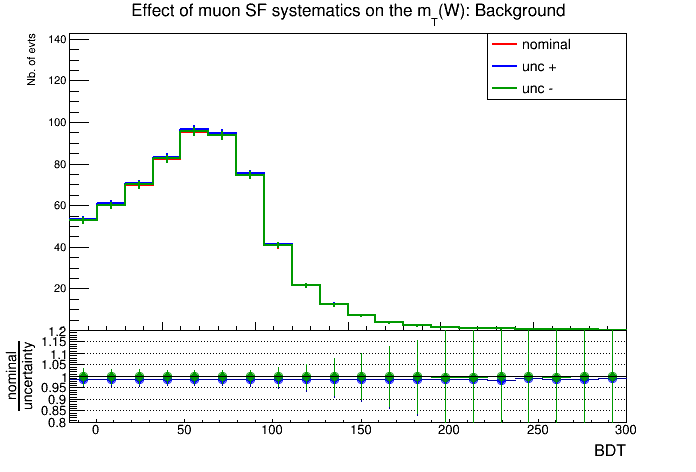
\includegraphics[width=0.48\textwidth]{Figures/boosteddecisiontrees/MTWsys/hist_mWt_muonSF_nom_bkg}
	\caption{Distribution of the nominal values and shift due to muon scale factors uncertainties for the transverse mass of the \PW\ boson in the \WZCR. All channel.}
	\label{fig:muonsfshiftmtWSTzct}
\end{figure}
\begin{figure}[h] 
	\centering
	% \subfigure[Background]{% \includegraphics[width=0.48\textwidth]{Figures/boosteddecisiontrees/singletopzct/systematics/hist_BDT_muonSF_nom_bkg}}
	% \subfigure[Signal]{% \includegraphics[width=0.48\textwidth]{Figures/boosteddecisiontrees/singletopzct/systematics/hist_BDT_muonSF_nom_sig}}
	\caption{Distribution of the nominal values and shift due to muon scale factor uncertainties for the BDT discriminant for the \Zct\ vertex in the \STSR. All channel.}
	\label{fig:muonsfshiftBDTSTzct}
\end{figure}
\begin{figure}[h] 
	\centering
	% \subfigure[Background]{% \includegraphics[width=0.48\textwidth]{Figures/boosteddecisiontrees/singletopzut/systematics/hist_BDT_muonSF_nom_bkg}}
	% \subfigure[Signal]{% \includegraphics[width=0.48\textwidth]{Figures/boosteddecisiontrees/singletopzut/systematics/hist_BDT_muonSF_nom_sig}}
	\caption{Distribution of the nominal values and shift due to muon scale factor uncertainties for the BDT discriminant for the \Zut\ vertex in the \STSR. All channel.}
	\label{fig:muonsfshiftBDTSTzut}
\end{figure}
\begin{figure}[h] 
	\centering
	% \subfigure[Background]{% \includegraphics[width=0.48\textwidth]{Figures/boosteddecisiontrees/toppairzct/systematics/hist_BDT_muonSF_nom_bkg}}
	% \subfigure[Signal]{% \includegraphics[width=0.48\textwidth]{Figures/boosteddecisiontrees/toppairzct/systematics/hist_BDT_muonSF_nom_sig}}
	\caption{Distribution of the nominal values and shift due to muon scale factor uncertainties for the BDT discriminant for the \Zct\ vertex in the \TTSR. All channel.}
	\label{fig:muonsfshiftBDTTTzct}
\end{figure}
\begin{figure}[h] 
	\centering
	% \subfigure[Background]{% \includegraphics[width=0.48\textwidth]{Figures/boosteddecisiontrees/toppairzut/systematics/hist_BDT_muonSF_nom_bkg}}
	% \subfigure[Signal]{% \includegraphics[width=0.48\textwidth]{Figures/boosteddecisiontrees/toppairzut/systematics/hist_BDT_muonSF_nom_sig}}
	\caption{Distribution of the nominal values and shift due to muon scale factor uncertainties for the BDT discriminant for the \Zut\ vertex in the \TTSR. All channel.}
	\label{fig:muonsfshiftBDTTTzut}
\end{figure}


\subsection{Effect of JES on the shapes}
\label{sec:JESsys}
\begin{figure}[h] 
	\centering 
	% 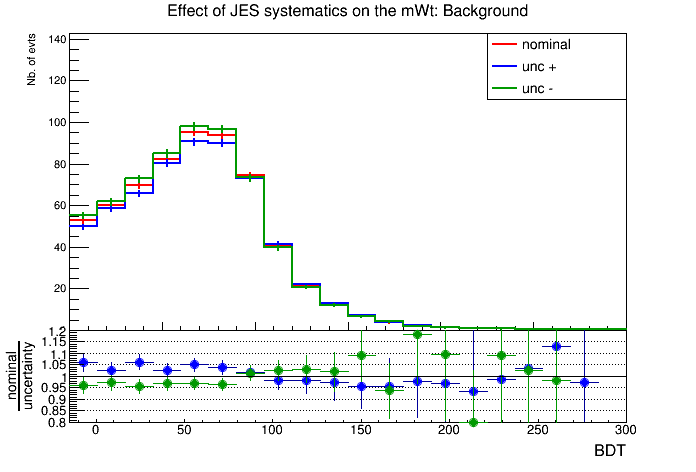
\includegraphics[width=0.48\textwidth]{Figures/boosteddecisiontrees/MTWsys/hist_mWt_JES_nom_bkg}
	\caption{Distribution of the nominal values and shift due to JES uncertainties for the transverse mass of the \PW\ boson in the \WZCR. All channel.}
	\label{fig:JESshiftmtWSTzct}
\end{figure}
\begin{figure}[h] 
	\centering
	% \subfigure[Background]{% \includegraphics[width=0.48\textwidth]{Figures/boosteddecisiontrees/singletopzct/systematics/hist_BDT_JES_nom_bkg}}
	% \subfigure[Signal]{% \includegraphics[width=0.48\textwidth]{Figures/boosteddecisiontrees/singletopzct/systematics/hist_BDT_JES_nom_sig}}
	\caption{Distribution of the nominal values and shift due to JES uncertainties for the BDT discriminant for the \Zct\ vertex in the \STSR. All channel.}
	\label{fig:JESshiftBDTSTzct}
\end{figure}
\begin{figure}[h] 
	\centering
	% \subfigure[Background]{% \includegraphics[width=0.48\textwidth]{Figures/boosteddecisiontrees/singletopzut/systematics/hist_BDT_JES_nom_bkg}}
	% \subfigure[Signal]{% \includegraphics[width=0.48\textwidth]{Figures/boosteddecisiontrees/singletopzut/systematics/hist_BDT_JES_nom_sig}}
	\caption{Distribution of the nominal values and shift due to JES uncertainties for the BDT discriminant for the \Zut\ vertex in the \STSR. All channel.}
	\label{fig:JESshiftBDTSTzut}
\end{figure}
\begin{figure}[h] 
	\centering
	% \subfigure[Background]{% \includegraphics[width=0.48\textwidth]{Figures/boosteddecisiontrees/toppairzct/systematics/hist_BDT_JES_nom_bkg}}
	% \subfigure[Signal]{% \includegraphics[width=0.48\textwidth]{Figures/boosteddecisiontrees/toppairzct/systematics/hist_BDT_JES_nom_sig}}
	\caption{Distribution of the nominal values and shift due to JES uncertainties for the BDT discriminant for the \Zct\ vertex in the \TTSR. All channel.}
	\label{fig:JESshiftBDTTTzct}
\end{figure}
\begin{figure}[h] 
	\centering
	% \subfigure[Background]{% \includegraphics[width=0.48\textwidth]{Figures/boosteddecisiontrees/toppairzut/systematics/hist_BDT_JES_nom_bkg}}
	% \subfigure[Signal]{% \includegraphics[width=0.48\textwidth]{Figures/boosteddecisiontrees/toppairzut/systematics/hist_BDT_JES_nom_sig}}
	\caption{Distribution of the nominal values and shift due to JES uncertainties for the BDT discriminant for the \Zut\ vertex in the \TTSR. All channel.}
	\label{fig:JESshiftBDTTTzut}
\end{figure}


\subsection{Effect of JER on the shapes}
\label{sec:JERsys}
\begin{figure}[h] 
	\centering 
	% \includegraphics[width=0.48\textwidth]{Figures/boosteddecisiontrees/MTWsys/hist_mWt_JER_nom_bkg}
	\caption{Distribution of the nominal values and shift due to JER uncertainties for the transverse mass of the \PW\ boson in the \WZCR. All channel.}
	\label{fig:JERshiftmtWSTzct}
\end{figure}
\begin{figure}[h] 
	\centering
	% \subfigure[Background]{% \includegraphics[width=0.48\textwidth]{Figures/boosteddecisiontrees/singletopzct/systematics/hist_BDT_JER_nom_bkg}}
	% \subfigure[Signal]{% \includegraphics[width=0.48\textwidth]{Figures/boosteddecisiontrees/singletopzct/systematics/hist_BDT_JER_nom_sig}}
	\caption{Distribution of the nominal values and shift due to JER uncertainties for the BDT discriminant for the \Zct\ vertex in the \STSR. All channel.}
	\label{fig:JERshiftBDTSTzct}
\end{figure}
\begin{figure}[h] 
	\centering
	% \subfigure[Background]{% \includegraphics[width=0.48\textwidth]{Figures/boosteddecisiontrees/singletopzut/systematics/hist_BDT_JER_nom_bkg}}
	% \subfigure[Signal]{% \includegraphics[width=0.48\textwidth]{Figures/boosteddecisiontrees/singletopzut/systematics/hist_BDT_JER_nom_sig}}
	\caption{Distribution of the nominal values and shift due to JER uncertainties for the BDT discriminant for the \Zut\ vertex in the \STSR. All channel.}
	\label{fig:JERshiftBDTSTzut}
\end{figure}
\begin{figure}[h] 
	\centering
	% \subfigure[Background]{% \includegraphics[width=0.48\textwidth]{Figures/boosteddecisiontrees/toppairzct/systematics/hist_BDT_JER_nom_bkg}}
	% \subfigure[Signal]{% \includegraphics[width=0.48\textwidth]{Figures/boosteddecisiontrees/toppairzct/systematics/hist_BDT_JER_nom_sig}}
	\caption{Distribution of the nominal values and shift due to JER uncertainties for the BDT discriminant for the \Zct\ vertex in the \TTSR. All channel.}
	\label{fig:JERshiftBDTTTzct}
\end{figure}
\begin{figure}[h] 
	\centering
	% \subfigure[Background]{% \includegraphics[width=0.48\textwidth]{Figures/boosteddecisiontrees/toppairzut/systematics/hist_BDT_JER_nom_bkg}}
	% \subfigure[Signal]{% \includegraphics[width=0.48\textwidth]{Figures/boosteddecisiontrees/toppairzut/systematics/hist_BDT_JER_nom_sig}}
	\caption{Distribution of the nominal values and shift due to JER uncertainties for the BDT discriminant for the \Zut\ vertex in the \TTSR. All channel.}
	\label{fig:JERshiftBDTTTzut}
\end{figure}



\subsection{Effect of b-tag scale factors on the shapes}
\label{sec:btagsys}
\begin{figure}[h] 
	\centering
	% \includegraphics[width=0.48\textwidth]{Figures/boosteddecisiontrees/MTWsys/hist_mWt_btagSF_cferr1_nom_bkg}
	\caption{Distribution of the nominal values and shift due to b tag cferr1 scale factors uncertainties for the transverse mass of the \PW\ boson in the \WZCR. All channel.}
	\label{fig:btagcferr1shiftmtWSTzct}
\end{figure}
\begin{figure}[h] 
	\centering
	% \subfigure[Background]{% \includegraphics[width=0.48\textwidth]{Figures/boosteddecisiontrees/singletopzct/systematics/hist_BDT_btagSF_cferr1_nom_bkg}}
	% \subfigure[Signal]{% \includegraphics[width=0.48\textwidth]{Figures/boosteddecisiontrees/singletopzct/systematics/hist_BDT_btagSF_cferr1_nom_sig}}
	\caption{Distribution of the nominal values and shift due to b tag cferr1 scale factor uncertainties for the BDT discriminant for the \Zct\ vertex in the \STSR. All channel.}
	\label{fig:btag_cferr1sfshiftBDTSTzct}
\end{figure}

\begin{figure}[h] 
	\centering
	% \subfigure[Background]{% \includegraphics[width=0.48\textwidth]{Figures/boosteddecisiontrees/singletopzut/systematics/hist_BDT_btagSF_cferr1_nom_bkg}}
	% \subfigure[Signal]{% \includegraphics[width=0.48\textwidth]{Figures/boosteddecisiontrees/singletopzut/systematics/hist_BDT_btagSF_cferr1_nom_sig}}
	\caption{Distribution of the nominal values and shift due to b tag cferr1 scale factor uncertainties for the BDT discriminant for the \Zut\ vertex in the \STSR. All channel.}
	\label{fig:btag_cferr1sfshiftBDTSTzut}
\end{figure}


\begin{figure}[h] 
	\centering
	% \subfigure[Background]{% \includegraphics[width=0.48\textwidth]{Figures/boosteddecisiontrees/toppairzct/systematics/hist_BDT_btagSF_cferr1_nom_bkg}}
	% \subfigure[Signal]{% \includegraphics[width=0.48\textwidth]{Figures/boosteddecisiontrees/toppairzct/systematics/hist_BDT_btagSF_cferr1_nom_sig}}
	\caption{Distribution of the nominal values and shift due to b tag cferr1 scale factor uncertainties for the BDT discriminant for the \Zct\ vertex in the \TTSR. All channel.}
	\label{fig:btag_cferr1sfshiftBDTTTzct}
\end{figure}


\begin{figure}[h] 
	\centering
	% \subfigure[Background]{% \includegraphics[width=0.48\textwidth]{Figures/boosteddecisiontrees/toppairzut/systematics/hist_BDT_btagSF_cferr1_nom_bkg}}
	% \subfigure[Signal]{% \includegraphics[width=0.48\textwidth]{Figures/boosteddecisiontrees/toppairzut/systematics/hist_BDT_btagSF_cferr1_nom_sig}}
	\caption{Distribution of the nominal values and shift due to b tag cferr1 scale factor uncertainties for the BDT discriminant for the \Zut\ vertex in the \TTSR. All channel.}
	\label{fig:btag_cferr1sfshiftBDTTTzut}
\end{figure}

\begin{figure}[h] 
	\centering
	% \includegraphics[width=0.48\textwidth]{Figures/boosteddecisiontrees/MTWsys/hist_mWt_btagSF_cferr2_nom_bkg}
	\caption{Distribution of the nominal values and shift due to b tag cferr2 scale factors uncertainties for the transverse mass of the \PW\ boson in the \WZCR. All channel.}
	\label{fig:btagcferr2shiftmtWSTzct}
\end{figure}

\begin{figure}[h] 
	\centering
	% \subfigure[Background]{% \includegraphics[width=0.48\textwidth]{Figures/boosteddecisiontrees/singletopzct/systematics/hist_BDT_btagSF_cferr2_nom_bkg}}
	% \subfigure[Signal]{% \includegraphics[width=0.48\textwidth]{Figures/boosteddecisiontrees/singletopzct/systematics/hist_BDT_btagSF_cferr2_nom_sig}}
	\caption{Distribution of the nominal values and shift due to b tag cferr2 scale factor uncertainties for the BDT discriminant for the \Zct\ vertex in the \STSR. All channel.}
	\label{fig:btag_cferr2sfshiftBDTSTzct}
\end{figure}


\begin{figure}[h] 
	\centering
	% \subfigure[Background]{% \includegraphics[width=0.48\textwidth]{Figures/boosteddecisiontrees/singletopzut/systematics/hist_BDT_btagSF_cferr2_nom_bkg}}
	% \subfigure[Signal]{% \includegraphics[width=0.48\textwidth]{Figures/boosteddecisiontrees/singletopzut/systematics/hist_BDT_btagSF_cferr2_nom_sig}}
	\caption{Distribution of the nominal values and shift due to b tag cferr2 scale factor uncertainties for the BDT discriminant for the \Zut\ vertex in the \STSR. All channel.}
	\label{fig:btag_cferr2sfshiftBDTSTzut}
\end{figure}

\begin{figure}[h] 
	\centering
	% \subfigure[Background]{% \includegraphics[width=0.48\textwidth]{Figures/boosteddecisiontrees/toppairzct/systematics/hist_BDT_btagSF_cferr2_nom_bkg}}
	% \subfigure[Signal]{% \includegraphics[width=0.48\textwidth]{Figures/boosteddecisiontrees/toppairzct/systematics/hist_BDT_btagSF_cferr2_nom_sig}}
	\caption{Distribution of the nominal values and shift due to b tag cferr2 scale factor uncertainties for the BDT discriminant for the \Zct\ vertex in the \TTSR. All channel.}
	\label{fig:btag_cferr2sfshiftBDTTTzct}
\end{figure}

\begin{figure}[h] 
	\centering
	% \subfigure[Background]{% \includegraphics[width=0.48\textwidth]{Figures/boosteddecisiontrees/toppairzut/systematics/hist_BDT_btagSF_cferr2_nom_bkg}}
	% \subfigure[Signal]{% \includegraphics[width=0.48\textwidth]{Figures/boosteddecisiontrees/toppairzut/systematics/hist_BDT_btagSF_cferr2_nom_sig}}
	\caption{Distribution of the nominal values and shift due to b tag cferr2 scale factor uncertainties for the BDT discriminant for the \Zut\ vertex in the \TTSR. All channel.}
	\label{fig:btag_cferr2sfshiftBDTTTzut}
\end{figure}

\begin{figure}[h] 
	\centering
	% \includegraphics[width=0.48\textwidth]{Figures/boosteddecisiontrees/MTWsys/hist_mWt_btagSF_hf_nom_bkg}
	\caption{Distribution of the nominal values and shift due to b tag hf scale factors uncertainties for the transverse mass of the \PW\ boson in the \WZCR. All channel.}
	\label{fig:btaghfshiftmtWSTzct}
\end{figure}
\begin{figure}[h] 
	\centering
	% \subfigure[Background]{% \includegraphics[width=0.48\textwidth]{Figures/boosteddecisiontrees/singletopzct/systematics/hist_BDT_btagSF_hf_nom_bkg}}
	% \subfigure[Signal]{% \includegraphics[width=0.48\textwidth]{Figures/boosteddecisiontrees/singletopzct/systematics/hist_BDT_btagSF_hf_nom_sig}}
	\caption{Distribution of the nominal values and shift due to b tag hf scale factor uncertainties for the BDT discriminant for the \Zct\ vertex in the \STSR. All channel.}
	\label{fig:btag_hfsfshiftBDTSTzct}
\end{figure}

\begin{figure}[h] 
	\centering
	% \subfigure[Background]{% \includegraphics[width=0.48\textwidth]{Figures/boosteddecisiontrees/singletopzut/systematics/hist_BDT_btagSF_hf_nom_bkg}}
	% \subfigure[Signal]{% \includegraphics[width=0.48\textwidth]{Figures/boosteddecisiontrees/singletopzut/systematics/hist_BDT_btagSF_hf_nom_sig}}
	\caption{Distribution of the nominal values and shift due to b tag hf scale factor uncertainties for the BDT discriminant for the \Zut\ vertex in the \STSR. All channel.}
	\label{fig:btag_hfsfshiftBDTSTzut}
\end{figure}

\begin{figure}[h] 
	\centering
	% \subfigure[Background]{% \includegraphics[width=0.48\textwidth]{Figures/boosteddecisiontrees/toppairzct/systematics/hist_BDT_btagSF_hf_nom_bkg}}
	% \subfigure[Signal]{% \includegraphics[width=0.48\textwidth]{Figures/boosteddecisiontrees/toppairzct/systematics/hist_BDT_btagSF_hf_nom_sig}}
	\caption{Distribution of the nominal values and shift due to b tag hf scale factor uncertainties for the BDT discriminant for the \Zct\ vertex in the \TTSR. All channel.}
	\label{fig:btag_hfsfshiftBDTTTzct}
\end{figure}

\begin{figure}[h] 
	\centering
	% \subfigure[Background]{% \includegraphics[width=0.48\textwidth]{Figures/boosteddecisiontrees/toppairzut/systematics/hist_BDT_btagSF_hf_nom_bkg}}
	% \subfigure[Signal]{% \includegraphics[width=0.48\textwidth]{Figures/boosteddecisiontrees/toppairzut/systematics/hist_BDT_btagSF_hf_nom_sig}}
	\caption{Distribution of the nominal values and shift due to b tag hf scale factor uncertainties for the BDT discriminant for the \Zut\ vertex in the \TTSR. All channel.}
	\label{fig:btag_hfsfshiftBDTTTzut}
\end{figure}
\begin{figure}[h] 
	\centering
	% \includegraphics[width=0.48\textwidth]{Figures/boosteddecisiontrees/MTWsys/hist_mWt_btagSF_hfstats1_nom_bkg}
	\caption{Distribution of the nominal values and shift due to b tag hfstats1 scale factors uncertainties for the transverse mass of the \PW\ boson in the \WZCR. All channel.}
	\label{fig:btaghfstats1shiftmtWSTzct}
\end{figure}
\begin{figure}[h] 
	\centering
	% \subfigure[Background]{% \includegraphics[width=0.48\textwidth]{Figures/boosteddecisiontrees/singletopzct/systematics/hist_BDT_btagSF_hfstats1_nom_bkg}}
	% \subfigure[Signal]{% \includegraphics[width=0.48\textwidth]{Figures/boosteddecisiontrees/singletopzct/systematics/hist_BDT_btagSF_hfstats1_nom_sig}}
	\caption{Distribution of the nominal values and shift due to b tag hfstats1 scale factor uncertainties for the BDT discriminant for the \Zct\ vertex in the \STSR. All channel.}
	\label{fig:btag_hfstats1sfshiftBDTSTzct}
\end{figure}

\begin{figure}[h] 
	\centering
	% \subfigure[Background]{% \includegraphics[width=0.48\textwidth]{Figures/boosteddecisiontrees/singletopzut/systematics/hist_BDT_btagSF_hfstats1_nom_bkg}}
	% \subfigure[Signal]{% \includegraphics[width=0.48\textwidth]{Figures/boosteddecisiontrees/singletopzut/systematics/hist_BDT_btagSF_hfstats1_nom_sig}}
	\caption{Distribution of the nominal values and shift due to b tag hfstats1 scale factor uncertainties for the BDT discriminant for the \Zut\ vertex in the \STSR. All channel.}
	\label{fig:btag_hfstats1sfshiftBDTSTzut}
\end{figure}

\begin{figure}[h] 
	\centering
	% \subfigure[Background]{% \includegraphics[width=0.48\textwidth]{Figures/boosteddecisiontrees/toppairzct/systematics/hist_BDT_btagSF_hfstats1_nom_bkg}}
	% \subfigure[Signal]{% \includegraphics[width=0.48\textwidth]{Figures/boosteddecisiontrees/toppairzct/systematics/hist_BDT_btagSF_hfstats1_nom_sig}}
	\caption{Distribution of the nominal values and shift due to b tag hfstats1 scale factor uncertainties for the BDT discriminant for the \Zct\ vertex in the \TTSR. All channel.}
	\label{fig:btag_hfstats1sfshiftBDTTTzct}
\end{figure}

\begin{figure}[h] 
	\centering
	% \subfigure[Background]{% \includegraphics[width=0.48\textwidth]{Figures/boosteddecisiontrees/toppairzut/systematics/hist_BDT_btagSF_hfstats1_nom_bkg}}
	% \subfigure[Signal]{% \includegraphics[width=0.48\textwidth]{Figures/boosteddecisiontrees/toppairzut/systematics/hist_BDT_btagSF_hfstats1_nom_sig}}
	\caption{Distribution of the nominal values and shift due to b tag hfstats1 scale factor uncertainties for the BDT discriminant for the \Zut\ vertex in the \TTSR. All channel.}
	\label{fig:btag_hfstats1sfshiftBDTTTzut}
\end{figure}
\begin{figure}[h] 
	\centering
	% \includegraphics[width=0.48\textwidth]{Figures/boosteddecisiontrees/MTWsys/hist_mWt_btagSF_hfstats2_nom_bkg}
	\caption{Distribution of the nominal values and shift due to b tag hfstats2 scale factors uncertainties for the transverse mass of the \PW\ boson in the \WZCR. All channel.}
	\label{fig:btaghfstats2shiftmtWSTzct}
\end{figure}
\begin{figure}[h] 
	\centering
	% \subfigure[Background]{% \includegraphics[width=0.48\textwidth]{Figures/boosteddecisiontrees/singletopzct/systematics/hist_BDT_btagSF_hfstats2_nom_bkg}}
	% \subfigure[Signal]{% \includegraphics[width=0.48\textwidth]{Figures/boosteddecisiontrees/singletopzct/systematics/hist_BDT_btagSF_hfstats2_nom_sig}}
	\caption{Distribution of the nominal values and shift due to b tag hfstats2 scale factor uncertainties for the BDT discriminant for the \Zct\ vertex in the \STSR. All channel.}
	\label{fig:btag_hfstats2sfshiftBDTSTzct}
\end{figure}

\begin{figure}[h] 
	\centering
	% \subfigure[Background]{% \includegraphics[width=0.48\textwidth]{Figures/boosteddecisiontrees/singletopzut/systematics/hist_BDT_btagSF_hfstats2_nom_bkg}}
	% \subfigure[Signal]{% \includegraphics[width=0.48\textwidth]{Figures/boosteddecisiontrees/singletopzut/systematics/hist_BDT_btagSF_hfstats2_nom_sig}}
	\caption{Distribution of the nominal values and shift due to b tag hfstats2 scale factor uncertainties for the BDT discriminant for the \Zut\ vertex in the \STSR. All channel.}
	\label{fig:btag_hfstats2sfshiftBDTSTzut}
\end{figure}

\begin{figure}[h] 
	\centering
	% \subfigure[Background]{% \includegraphics[width=0.48\textwidth]{Figures/boosteddecisiontrees/toppairzct/systematics/hist_BDT_btagSF_hfstats2_nom_bkg}}
	% \subfigure[Signal]{% \includegraphics[width=0.48\textwidth]{Figures/boosteddecisiontrees/toppairzct/systematics/hist_BDT_btagSF_hfstats2_nom_sig}}
	\caption{Distribution of the nominal values and shift due to b tag hfstats2 scale factor uncertainties for the BDT discriminant for the \Zct\ vertex in the \TTSR. All channel.}
	\label{fig:btag_hfstats2sfshiftBDTTTzct}
\end{figure}

\begin{figure}[h] 
	\centering
	% \subfigure[Background]{% \includegraphics[width=0.48\textwidth]{Figures/boosteddecisiontrees/toppairzut/systematics/hist_BDT_btagSF_hfstats2_nom_bkg}}
	% \subfigure[Signal]{% \includegraphics[width=0.48\textwidth]{Figures/boosteddecisiontrees/toppairzut/systematics/hist_BDT_btagSF_hfstats2_nom_sig}}
	\caption{Distribution of the nominal values and shift due to b tag hfstats2 scale factor uncertainties for the BDT discriminant for the \Zut\ vertex in the \TTSR. All channel.}
	\label{fig:btag_hfstats2sfshiftBDTTTzut}
\end{figure}



\begin{figure}[h] 
	\centering
	% \includegraphics[width=0.48\textwidth]{Figures/boosteddecisiontrees/MTWsys/hist_mWt_btagSF_lf_nom_bkg}
	\caption{Distribution of the nominal values and shift due to b tag lf scale factors uncertainties for the transverse mass of the \PW\ boson in the \WZCR. All channel.}
	\label{fig:btaglfshiftmtWSTzct}
\end{figure}
\begin{figure}[h] 
	\centering
	% \subfigure[Background]{% \includegraphics[width=0.48\textwidth]{Figures/boosteddecisiontrees/singletopzct/systematics/hist_BDT_btagSF_lf_nom_bkg}}
	% \subfigure[Signal]{% \includegraphics[width=0.48\textwidth]{Figures/boosteddecisiontrees/singletopzct/systematics/hist_BDT_btagSF_lf_nom_sig}}
	\caption{Distribution of the nominal values and shift due to b tag lf scale factor uncertainties for the BDT discriminant for the \Zct\ vertex in the \STSR. All channel.}
	\label{fig:btag_lfsfshiftBDTSTzct}
\end{figure}

\begin{figure}[h] 
	\centering
	% \subfigure[Background]{% \includegraphics[width=0.48\textwidth]{Figures/boosteddecisiontrees/singletopzut/systematics/hist_BDT_btagSF_lf_nom_bkg}}
	% \subfigure[Signal]{% \includegraphics[width=0.48\textwidth]{Figures/boosteddecisiontrees/singletopzut/systematics/hist_BDT_btagSF_lf_nom_sig}}
	\caption{Distribution of the nominal values and shift due to b tag lf scale factor uncertainties for the BDT discriminant for the \Zut\ vertex in the \STSR. All channel.}
	\label{fig:btag_lfsfshiftBDTSTzut}
\end{figure}

\begin{figure}[h] 
	\centering
	% \subfigure[Background]{% \includegraphics[width=0.48\textwidth]{Figures/boosteddecisiontrees/toppairzct/systematics/hist_BDT_btagSF_lf_nom_bkg}}
	% \subfigure[Signal]{% \includegraphics[width=0.48\textwidth]{Figures/boosteddecisiontrees/toppairzct/systematics/hist_BDT_btagSF_lf_nom_sig}}
	\caption{Distribution of the nominal values and shift due to b tag lf scale factor uncertainties for the BDT discriminant for the \Zct\ vertex in the \TTSR. All channel.}
	\label{fig:btag_lfsfshiftBDTTTzct}
\end{figure}


\begin{figure}[h] 
	\centering
	% \subfigure[Background]{% \includegraphics[width=0.48\textwidth]{Figures/boosteddecisiontrees/toppairzut/systematics/hist_BDT_btagSF_lf_nom_bkg}}
	% \subfigure[Signal]{% \includegraphics[width=0.48\textwidth]{Figures/boosteddecisiontrees/toppairzut/systematics/hist_BDT_btagSF_lf_nom_sig}}
	\caption{Distribution of the nominal values and shift due to b tag lf scale factor uncertainties for the BDT discriminant for the \Zut\ vertex in the \TTSR. All channel.}
	\label{fig:btag_lfsfshiftBDTTTzut}
\end{figure}
\begin{figure}[h] 
	\centering
	% \includegraphics[width=0.48\textwidth]{Figures/boosteddecisiontrees/MTWsys/hist_mWt_btagSF_lfstats1_nom_bkg}
	\caption{Distribution of the nominal values and shift due to b tag lfstats1 scale factors uncertainties for the transverse mass of the \PW\ boson in the \WZCR. All channel.}
	\label{fig:btaglfstats1shiftmtWSTzct}
\end{figure}
\begin{figure}[h] 
	\centering
	% \subfigure[Background]{% \includegraphics[width=0.48\textwidth]{Figures/boosteddecisiontrees/singletopzct/systematics/hist_BDT_btagSF_lfstats1_nom_bkg}}
	% \subfigure[Signal]{% \includegraphics[width=0.48\textwidth]{Figures/boosteddecisiontrees/singletopzct/systematics/hist_BDT_btagSF_lfstats1_nom_sig}}
	\caption{Distribution of the nominal values and shift due to b tag lfstats1 scale factor uncertainties for the BDT discriminant for the \Zct\ vertex in the \STSR. All channel.}
	\label{fig:btag_lfstats1sfshiftBDTSTzct}
\end{figure}

\begin{figure}[h] 
	\centering
	% \subfigure[Background]{% \includegraphics[width=0.48\textwidth]{Figures/boosteddecisiontrees/singletopzut/systematics/hist_BDT_btagSF_lfstats1_nom_bkg}}
	% \subfigure[Signal]{% \includegraphics[width=0.48\textwidth]{Figures/boosteddecisiontrees/singletopzut/systematics/hist_BDT_btagSF_lfstats1_nom_sig}}
	\caption{Distribution of the nominal values and shift due to b tag lfstats1 scale factor uncertainties for the BDT discriminant for the \Zut\ vertex in the \STSR. All channel.}
	\label{fig:btag_lfstats1sfshiftBDTSTzut}
\end{figure}

\begin{figure}[h] 
	\centering
	% \subfigure[Background]{% \includegraphics[width=0.48\textwidth]{Figures/boosteddecisiontrees/toppairzct/systematics/hist_BDT_btagSF_lfstats1_nom_bkg}}
	% \subfigure[Signal]{% \includegraphics[width=0.48\textwidth]{Figures/boosteddecisiontrees/toppairzct/systematics/hist_BDT_btagSF_lfstats1_nom_sig}}
	\caption{Distribution of the nominal values and shift due to b tag lfstats1 scale factor uncertainties for the BDT discriminant for the \Zct\ vertex in the \TTSR. All channel.}
	\label{fig:btag_lfstats1sfshiftBDTTTzct}
\end{figure}

\begin{figure}[h] 
	\centering
	% \subfigure[Background]{% \includegraphics[width=0.48\textwidth]{Figures/boosteddecisiontrees/toppairzut/systematics/hist_BDT_btagSF_lfstats1_nom_bkg}}
	% \subfigure[Signal]{% \includegraphics[width=0.48\textwidth]{Figures/boosteddecisiontrees/toppairzut/systematics/hist_BDT_btagSF_lfstats1_nom_sig}}
	\caption{Distribution of the nominal values and shift due to b tag lfstats1 scale factor uncertainties for the BDT discriminant for the \Zut\ vertex in the \TTSR. All channel.}
	\label{fig:btag_lfstats1sfshiftBDTTTzut}
\end{figure}
\begin{figure}[h] 
	\centering
	% \includegraphics[width=0.48\textwidth]{Figures/boosteddecisiontrees/MTWsys/hist_mWt_btagSF_lfstats2_nom_bkg}
	\caption{Distribution of the nominal values and shift due to b tag lfstats2 scale factors uncertainties for the transverse mass of the \PW\ boson in the \WZCR. All channel.}
	\label{fig:btaglfstats2shiftmtWSTzct}
\end{figure}
\begin{figure}[h] 
	\centering
	% \subfigure[Background]{% \includegraphics[width=0.48\textwidth]{Figures/boosteddecisiontrees/singletopzct/systematics/hist_BDT_btagSF_lfstats2_nom_bkg}}
	% \subfigure[Signal]{% \includegraphics[width=0.48\textwidth]{Figures/boosteddecisiontrees/singletopzct/systematics/hist_BDT_btagSF_lfstats2_nom_sig}}
	\caption{Distribution of the nominal values and shift due to b tag lfstats2 scale factor uncertainties for the BDT discriminant for the \Zct\ vertex in the \STSR. All channel.}
	\label{fig:btag_lfstats2sfshiftBDTSTzct}
\end{figure}

\begin{figure}[h] 
	\centering
	% \subfigure[Background]{% \includegraphics[width=0.48\textwidth]{Figures/boosteddecisiontrees/singletopzut/systematics/hist_BDT_btagSF_lfstats2_nom_bkg}}
	% \subfigure[Signal]{% \includegraphics[width=0.48\textwidth]{Figures/boosteddecisiontrees/singletopzut/systematics/hist_BDT_btagSF_lfstats2_nom_sig}}
	\caption{Distribution of the nominal values and shift due to b tag lfstats2 scale factor uncertainties for the BDT discriminant for the \Zut\ vertex in the \STSR. All channel.}
	\label{fig:btag_lfstats2sfshiftBDTSTzut}
\end{figure}

\begin{figure}[h] 
	\centering
	% \subfigure[Background]{% \includegraphics[width=0.48\textwidth]{Figures/boosteddecisiontrees/toppairzct/systematics/hist_BDT_btagSF_lfstats2_nom_bkg}}
	% \subfigure[Signal]{% \includegraphics[width=0.48\textwidth]{Figures/boosteddecisiontrees/toppairzct/systematics/hist_BDT_btagSF_lfstats2_nom_sig}}
	\caption{Distribution of the nominal values and shift due to b tag lfstats2 scale factor uncertainties for the BDT discriminant for the \Zct\ vertex in the \TTSR. All channel.}
	\label{fig:btag_lfstats2sfshiftBDTTTzct}
\end{figure}

\begin{figure}[h] 
	\centering
	% \subfigure[Background]{% \includegraphics[width=0.48\textwidth]{Figures/boosteddecisiontrees/toppairzut/systematics/hist_BDT_btagSF_lfstats2_nom_bkg}}
	% \subfigure[Signal]{% \includegraphics[width=0.48\textwidth]{Figures/boosteddecisiontrees/toppairzut/systematics/hist_BDT_btagSF_lfstats2_nom_sig}}
	\caption{Distribution of the nominal values and shift due to b tag lfstats2 scale factor uncertainties for the BDT discriminant for the \Zut\ vertex in the \TTSR. All channel.}
	\label{fig:btag_lfstats2sfshiftBDTTTzut}
\end{figure}
\end{comment}
\section{Limit setting procedure validation}
The analysis strategy has been established using a blinded strategy. Through the use of a pseudo dataset, the limit setting procedure has been validated. Signal injection tests for which the signal strength from a pseudo dataset with a pre-set  signal strength is estimated are perfomed and shown in \fig{fig:plotzut}.
\begin{figure}[ht]
	\centering
	 \includegraphics[width=0.49\linewidth]{6_Search/Figures/SignalInjection/plotZut}
	 \includegraphics[width=0.49\linewidth]{6_Search/Figures/SignalInjection/plotZct}
	\caption{The  obtained signal strength with the Maximum Likelihood method is in agreement with the signal strength used to generate the Asimov data set for the \Zut\ (left) and \Zct\ (right) couplings.}
	\label{fig:plotzut}
\end{figure}

Another validation has been done by performing a Maximum Likelihood fit in the \WZCR\ only, considering all lepton channels. A simultaneous fit of the signal strength of the \NPE, \NPM\ and the \WZ+jets backgrounds is done by using the multi-dimensional fit in \texttt{Higgs} \texttt{Combine} \texttt{Tool}. The resulting signal strengths can then be applied on the distribution o f the transverse mass of the \PW\ boson to verify data/MC agreement, as can be seen in Fig. \ref{fig:mtwstack}. Furthermore, a goodness of fit test is performed, resulting in a p-value of 0.3 (see Fig. \ref{fig:gof} ) .

\begin{figure}[htbp]
	\centering
	 \includegraphics[width=0.7\linewidth]{6_Search/Figures/GOF/GOF_1000toys}
	\caption{Goodness of fit testing in the \WZCR\  with 1000 toys. The likelihood ration is denoted as $\lambda$.}
	\label{fig:gof}
\end{figure}

\begin{figure}[htbp]
	\centering
 \includegraphics[width=0.49\linewidth]{6_Search/Figures/WZcontrol/wzcontrol_MVA_mWt_uuu_Stack}
	 \includegraphics[width=0.49\linewidth]{6_Search/Figures/WZcontrol/wzcontrol_MVA_mWt_uue_Stack}
 \includegraphics[width=0.49\linewidth]{6_Search/Figures/WZcontrol/wzcontrol_MVA_mWt_eeu_Stack}
	 \includegraphics[width=0.49\linewidth]{6_Search/Figures/WZcontrol/wzcontrol_MVA_mWt_eee_Stack}
	\caption{The transverse mass of the \PW\ boson in the \WZCR\ for the \mumumu\ channel (left, upper), \emumu\ channel (right, upper), \eemu\ channel (left, lower), and 3 electrons channel (right, lower).}
	\label{fig:mtwstack}
\end{figure}
\newpage
Using the normalisations obtained by fitting the \WZCR\ only,  one can look at the data/MC  agreement in the \WZCR\ for all the variables used to create the BDT variables. These show good agreement as illustrated in \fig{fig:agreement}.

\begin{comment}
%\begin{figure}[htbp]
%	\centering \begin{minipage}{0.45\textwidth} \centering
%		% % \includegraphics[width=1.\linewidth]{FiguresAfterUnblinding/WZcontrol/wzcontrol_MVA_SMtop_eta_all_Stack}
%		\caption{Pseudo rapidity of the \SM\ top in the \WZCR\ for the sum of the different lepton channels after the initial normalization fit. }
%		\label{fig:allwzcontrolmvasmtopeta}
%	\end{minipage} 
%	\hfill
%	\begin{minipage}{0.45\textwidth} \centering
%		% % \includegraphics[width=1.\linewidth]{FiguresAfterUnblinding/WZcontrol/wzcontrol_MVA_mlb_all_Stack}
%		\caption{Invariant mass of the \SM\ \Pbottom\ jet and \PW\ lepton in the \WZCR\ for the sum of the different lepton channels after the initial normalization fit.}
%		\label{fig:allwzcontrolmvamlb}
%	\end{minipage} 
%	\hfill
%	\begin{minipage}{0.45\textwidth} \centering
%		% % \includegraphics[width=1.\linewidth]{FiguresAfterUnblinding/WZcontrol/wzcontrol_MVA_dPhiWlepb_all_Stack}
%		\caption{$\Delta \Phi$ between the \PW\ lepton and the \SM\ \Pbottom\ jet in the \WZCR\ for the sum of the different lepton channels after the initial normalization fit.}
%		\label{fig:allwzcontrolmvadPhiWlepb}
%	\end{minipage} 
%	\hfill
%	\begin{minipage}{0.45\textwidth} \centering
%		% % \includegraphics[width=1.\linewidth]{FiguresAfterUnblinding/WZcontrol/wzcontrol_MVA_deltaRWlepJet_min_all_Stack}
%		\caption{minimal $\Delta R$ between the \PW\ lepton and jets in the \WZCR\ for the sum of the different lepton channels after the initial normalization fit.}
%		\label{fig:allwzcontrolmvaMVA_deltaRWlepJet_min}
%	\end{minipage}
%\end{figure}
%
%\begin{figure}[ht]
%	\centering 
%	\begin{minipage}{0.45\textwidth} \centering
%		% % \includegraphics[width=1.\linewidth]{FiguresAfterUnblinding/WZcontrol/wzcontrol_MVA_Zboson_M_all_Stack}
%		\caption{Invariant mass of the \PZ\ boson in the \WZCR\ for the sum of the different lepton channels after the initial normalization fit.}
%		\label{fig:allwzcontrolmvaZbosonM}
%	\end{minipage} 
%	\hfill
%	\begin{minipage}{0.45\textwidth} \centering
%		% % \includegraphics[width=1.\linewidth]{FiguresAfterUnblinding/WZcontrol/wzcontrol_MVA_dPhiZWlep_all_Stack}
%		\caption{$\Delta \Phi$ between the \PW\ lepton and the \PZ\ boson in the \WZCR\ for the sum of the different lepton channels after the initial normalization fit.}
%		\label{fig:allwzcontrolmvadPhiZWlep}
%	\end{minipage} 
%	
%	\hfill
%	\begin{minipage}{0.45\textwidth} \centering
%		% % \includegraphics[width=1.\linewidth]{FiguresAfterUnblinding/WZcontrol/wzcontrol_MVA_dRWlepb_all_Stack}
%		\caption{$\Delta R$ between the \PW\ lepton and the \SM\ \Pbottom\ jet in the \WZCR\ for the sum of the different lepton channels after the initial normalization fit.}
%		\label{fig:allwzcontrolmvadRWlepb}
%	\end{minipage} 
%	\hfill
%	\begin{minipage}{0.45\textwidth} \centering
%		% % \includegraphics[width=1.\linewidth]{FiguresAfterUnblinding/WZcontrol/wzcontrol_MVA_NJets_CSVv2M_all_Stack}
%		\caption{Number of b jets according to the CSVv2 medium working point in the \WZCR\ for the sum of the different lepton channels after the initial normalization fit.}
%		\label{fig:allwzcontrolmvaNJets_CSVv2M}
%	\end{minipage}
%\end{figure}
%\newpage
%\begin{figure}[ht]
%	\centering \begin{minipage}{0.45\textwidth} \centering
%		% % \includegraphics[width=1.\linewidth]{FiguresAfterUnblinding/WZcontrol/wzcontrol_MVA_FCNCtop_M_all_Stack}
%		\caption{Invariant mass of the FCNC top in the \WZCR\ for the sum of the different lepton channels after the initial normalization fit. }
%		\label{fig:allwzcontrolmvaFCNCtop_M}
%	\end{minipage} \hfill
%	\begin{minipage}{0.45\textwidth} \centering
%		% % \includegraphics[width=1.\linewidth]{FiguresAfterUnblinding/WZcontrol/wzcontrol_MVA_dRZc_all_Stack}
%		\caption{$\Delta R$ between the \PZ\ boson and the FCNC light jet in the \WZCR\ for the sum of the different lepton channels after the initial normalization fit. }
%		\label{fig:allwzcontrolmvadRZc}
%	\end{minipage} \hfill
%	\begin{minipage}{0.45\textwidth} \centering
%		% % \includegraphics[width=1.\linewidth]{FiguresAfterUnblinding/WZcontrol/wzcontrol_MVA_dRSMjetLightjet_all_Stack}
%		\caption{$\Delta R$ between the \SM\ jet and the FCNC jet in the \WZCR\ for the sum of the different lepton channels after the initial normalization fit. }
%		\label{fig:allwzcontrolmvadRSMjetLightjet}
%	\end{minipage} \hfill
%	\begin{minipage}{0.45\textwidth} \centering
%		% % \includegraphics[width=1.\linewidth]{FiguresAfterUnblinding/WZcontrol/wzcontrol_MVA_charge_asym_all_Stack}
%		\caption{Charge of the \PW\ lepton times the absolute pseudo rapidity of the \PW\ lepton in the \WZCR\ for the sum of the different lepton channels after the initial normalization fit. }
%		\label{fig:allwzcontrolmvachargeasym}
%	\end{minipage} 
%\end{figure}
%\begin{figure}[ht]
%	\centering \begin{minipage}{0.45\textwidth} \centering
%		% % \includegraphics[width=1.\linewidth]{FiguresAfterUnblinding/WZcontrol/wzcontrol_MVA_bdiscCSVv2_jet_0_all_Stack}
%		\caption{b discriminant of the highest $p_T$ jet in the \WZCR\ for the sum of the different lepton channels after the initial normalization fit.}
%		\label{fig:allwzcontrolmvabdis}
%	\end{minipage} \hfill
%	\begin{minipage}{0.45\textwidth} \centering
%		% % \includegraphics[width=1.\linewidth]{FiguresAfterUnblinding/WZcontrol/wzcontrol_MVA_TotalHt_lep_all_Stack}
%		\caption{Total Ht of the leptons in the \WZCR\ for the sum of the different lepton channels after the initial normalization fit.}
%		\label{fig:allwzcontrolmvaht}
%	\end{minipage} \hfill
%	\begin{minipage}{0.45\textwidth} \centering
%		% % \includegraphics[width=1.\linewidth]{FiguresAfterUnblinding/WZcontrol/wzcontrol_MVA_ptWQ_all_Stack}
%		\caption{The $p_T$ of the \PW\ lepton times its charge in the \WZCR\ for the sum of the different lepton channels after the initial normalization fit. }
%		\label{fig:allwzcontrolmvaptwq}
%	\end{minipage} \hfill
%	\begin{minipage}{0.45\textwidth} \centering
%		% % \includegraphics[width=1.\linewidth]{FiguresAfterUnblinding/WZcontrol/wzcontrol_MVA_TotalInvMass_lep_all_Stack}
%		\caption{The total invariant mass of the leptons in the \WZCR\ for the sum of the different lepton channels after the initial normalization fit. }
%		\label{fig:allwzcontrolmvam3l}
%	\end{minipage} 
%\end{figure}
%\begin{figure}[ht]
%	\centering \begin{minipage}{0.45\textwidth} \centering
%		% % \includegraphics[width=1.\linewidth]{FiguresAfterUnblinding/WZcontrol/wzcontrol_MVA_dRZWlep_all_Stack}
%		\caption{$\Delta R$ between the \PW\ lepton and the \PZ\ boson in the \WZCR\ for the sum of the different lepton channels after the initial normalization fit.}
%		\label{fig:allwzcontrolmvadRZWlep}
%	\end{minipage} \hfill
%	\begin{minipage}{0.45\textwidth} \centering
%		% % \includegraphics[width=1.\linewidth]{FiguresAfterUnblinding/WZcontrol/wzcontrol_MVA_TotalInvMass_all_Stack}
%		\caption{The total invariant mass of the event in the \WZCR\ for the sum of the different lepton channels after the initial normalization fit. }
%		\label{fig:allwzcontrolmvainvmass}
%	\end{minipage} \hfill
%	\begin{minipage}{0.45\textwidth} \centering
%		% % \includegraphics[width=1.\linewidth]{FiguresAfterUnblinding/WZcontrol/wzcontrol_MVA_Bdis_LightJet_all_Stack}
%		\caption{The b discriminant of the FCNC jet in the \WZCR\ for the sum of the different lepton channels after the initial normalization fit. }
%		\label{fig:allwzcontrolmvabdislightjet}
%	\end{minipage} \hfill
%	\begin{minipage}{0.45\textwidth} \centering
%		% % \includegraphics[width=1.\linewidth]{FiguresAfterUnblinding/WZcontrol/wzcontrol_MVA_dRZb_all_Stack}
%		\caption{$\Delta R$ between the \PZ\ boson and the \SM\ \Pbottom\ jet in the \WZCR\ for the sum of the different lepton channels after the initial normalization fit. }
%		\label{fig:allwzcontrolmvadRZb}
%	\end{minipage} 
%\end{figure}

%\subsection*{\STSR}
%\begin{figure}[ht]
%	\centering \begin{minipage}{0.45\textwidth} \centering
%		% % \includegraphics[width=1.\linewidth]{FiguresAfterUnblinding/STSR/singletop_MVA_SMtop_eta_all_Stack}
%		\caption{Pseudo rapidity of the \SM\ top in the \STSR\ for the sum of the different lepton channels after the initial normalization fit. }
%		\label{fig:allsingletopmvasmtopeta}
%	\end{minipage} 
%	\hfill
%	\begin{minipage}{0.45\textwidth} \centering
%		% % \includegraphics[width=1.\linewidth]{FiguresAfterUnblinding/STSR/singletop_MVA_mlb_all_Stack}
%		\caption{Invariant mass of the \SM\ \Pbottom\ jet and \PW\ lepton in the \STSR\ for the sum of the different lepton channels after the initial normalization fit.}
%		\label{fig:allsingletopmvamlb}
%	\end{minipage} 
%	\hfill
%	\begin{minipage}{0.45\textwidth} \centering
%		% % \includegraphics[width=1.\linewidth]{FiguresAfterUnblinding/STSR/singletop_MVA_dPhiWlepb_all_Stack}
%		\caption{$\Delta \Phi$ between the \PW\ lepton and the \SM\ \Pbottom\ jet in the \STSR\ for the sum of the different lepton channels after the initial normalization fit.}
%		\label{fig:allsingletopmvadPhiWlepb}
%	\end{minipage} 
%	\hfill
%	\begin{minipage}{0.45\textwidth} \centering
%		% % \includegraphics[width=1.\linewidth]{FiguresAfterUnblinding/STSR/singletop_MVA_deltaRWlepJet_min_all_Stack}
%		\caption{minimal $\Delta R$ between the \PW\ lepton and jets in the \STSR\ for the sum of the different lepton channels after the initial normalization fit.}
%		\label{fig:allsingletopmvaMVA_deltaRWlepJet_min}
%	\end{minipage}
%\end{figure}
%\newpage
%\begin{figure}[ht]
%	\centering 
%	\begin{minipage}{0.45\textwidth} \centering
%		% % \includegraphics[width=1.\linewidth]{FiguresAfterUnblinding/STSR/singletop_MVA_Zboson_M_all_Stack}
%		\caption{Invariant mass of the \PZ\ boson in the \STSR\ for the sum of the different lepton channels after the initial normalization fit.}
%		\label{fig:allsingletopmvaZbosonM}
%	\end{minipage} 
%	\hfill
%	\begin{minipage}{0.45\textwidth} \centering
%		% % \includegraphics[width=1.\linewidth]{FiguresAfterUnblinding/STSR/singletop_MVA_dPhiZWlep_all_Stack}
%		\caption{$\Delta \Phi$ between the \PW\ lepton and the \PZ\ boson in the \STSR\ for the sum of the different lepton channels after the initial normalization fit.}
%		\label{fig:allsingletopmvadPhiZWlep}
%	\end{minipage} 
%	
%	\hfill
%	\begin{minipage}{0.45\textwidth} \centering
%		% % \includegraphics[width=1.\linewidth]{FiguresAfterUnblinding/STSR/singletop_MVA_dRWlepb_all_Stack}
%		\caption{$\Delta R$ between the \PW\ lepton and the \SM\ \Pbottom\ jet in the \STSR\ for the sum of the different lepton channels after the initial normalization fit.}
%		\label{fig:allsingletopmvadRWlepb}
%	\end{minipage} 
%	\hfill
%	\begin{minipage}{0.45\textwidth} \centering
%		% % \includegraphics[width=1.\linewidth]{FiguresAfterUnblinding/STSR/singletop_MVA_NJets_CSVv2M_all_Stack}
%		\caption{Number of b jets according to the CSVv2 medium working point in the \STSR\ for the sum of the different lepton channels after the initial normalization fit.}
%		\label{fig:allsingletopmvaNJets_CSVv2M}
%	\end{minipage}
%\end{figure}
%\newpage
%\begin{figure}[ht]
%	\centering \begin{minipage}{0.45\textwidth} \centering
%		% % \includegraphics[width=1.\linewidth]{FiguresAfterUnblinding/STSR/singletop_MVA_FCNCtop_M_all_Stack}
%		\caption{Invariant mass of the FCNC top in the \STSR\ for the sum of the different lepton channels after the initial normalization fit. }
%		\label{fig:allsingletopmvaFCNCtop_M}
%	\end{minipage} \hfill
%	\begin{minipage}{0.45\textwidth} \centering
%		% % \includegraphics[width=1.\linewidth]{FiguresAfterUnblinding/STSR/singletop_MVA_dRZc_all_Stack}
%		\caption{$\Delta R$ between the \PZ\ boson and the FCNC light jet in the \STSR\ for the sum of the different lepton channels after the initial normalization fit. }
%		\label{fig:allsingletopmvadRZc}
%	\end{minipage} \hfill
%	\begin{minipage}{0.45\textwidth} \centering
%		% % \includegraphics[width=1.\linewidth]{FiguresAfterUnblinding/STSR/singletop_MVA_dRSMjetLightjet_all_Stack}
%		\caption{$\Delta R$ between the \SM\ jet and the FCNC jet in the \STSR\ for the sum of the different lepton channels after the initial normalization fit. }
%		\label{fig:allsingletopmvadRSMjetLightjet}
%	\end{minipage} \hfill
%	\begin{minipage}{0.45\textwidth} \centering
%		% % \includegraphics[width=1.\linewidth]{FiguresAfterUnblinding/STSR/singletop_MVA_charge_asym_all_Stack}
%		\caption{Charge of the \PW\ lepton times the absolute pseudo rapidity of the \PW\ lepton in the \STSR\ for the sum of the different lepton channels after the initial normalization fit. }
%		\label{fig:allsingletopmvachargeasym}
%	\end{minipage} 
%\end{figure}
%\begin{figure}[ht]
%	\centering \begin{minipage}{0.45\textwidth} \centering
%		% % \includegraphics[width=1.\linewidth]{FiguresAfterUnblinding/STSR/singletop_MVA_bdiscCSVv2_jet_0_all_Stack}
%		\caption{b discriminant of the highest $p_T$ jet in the \STSR\ for the sum of the different lepton channels after the initial normalization fit.}
%		\label{fig:allsingletopmvabdis}
%	\end{minipage} \hfill
%	\begin{minipage}{0.45\textwidth} \centering
%		% % \includegraphics[width=1.\linewidth]{FiguresAfterUnblinding/STSR/singletop_MVA_TotalHt_lep_all_Stack}
%		\caption{Total Ht of the leptons in the \STSR\ for the sum of the different lepton channels after the initial normalization fit.}
%		\label{fig:allsingletopmvaht}
%	\end{minipage} \hfill
%	\begin{minipage}{0.45\textwidth} \centering
%		% % \includegraphics[width=1.\linewidth]{FiguresAfterUnblinding/STSR/singletop_MVA_ptWQ_all_Stack}
%		\caption{The $p_T$ of the \PW\ lepton times its charge in the \STSR\ for the sum of the different lepton channels after the initial normalization fit. }
%		\label{fig:allsingletopmvaptwq}
%	\end{minipage} \hfill
%	\begin{minipage}{0.45\textwidth} \centering
%		% % \includegraphics[width=1.\linewidth]{FiguresAfterUnblinding/STSR/singletop_MVA_TotalInvMass_lep_all_Stack}
%		\caption{The total invariant mass of the leptons in the \STSR\ for the sum of the different lepton channels after the initial normalization fit. }
%		\label{fig:allsingletopmvam3l}
%	\end{minipage} 
%\end{figure}
%\begin{figure}[ht]
%	\centering \begin{minipage}{0.45\textwidth} \centering
%		% % \includegraphics[width=1.\linewidth]{FiguresAfterUnblinding/STSR/singletop_MVA_dRZWlep_all_Stack}
%		\caption{$\Delta R$ between the \PW\ lepton and the \PZ\ boson in the \STSR\ for the sum of the different lepton channels after the initial normalization fit.}
%		\label{fig:allsingletopmvadRZWlep}
%	\end{minipage} \hfill
%	\begin{minipage}{0.45\textwidth} \centering
%		% % \includegraphics[width=1.\linewidth]{FiguresAfterUnblinding/STSR/singletop_MVA_TotalInvMass_all_Stack}
%		\caption{The total invariant mass of the event in the \STSR\ for the sum of the different lepton channels after the initial normalization fit. }
%		\label{fig:allsingletopmvainvmass}
%	\end{minipage} \hfill
%	\begin{minipage}{0.45\textwidth} \centering
%		% % \includegraphics[width=1.\linewidth]{FiguresAfterUnblinding/STSR/singletop_MVA_Bdis_LightJet_all_Stack}
%		\caption{The b discriminant of the FCNC jet in the \STSR\ for the sum of the different lepton channels after the initial normalization fit. }
%		\label{fig:allsingletopmvabdislightjet}
%	\end{minipage} \hfill
%	\begin{minipage}{0.45\textwidth} \centering
%		% % \includegraphics[width=1.\linewidth]{FiguresAfterUnblinding/STSR/singletop_MVA_dRZb_all_Stack}
%		\caption{$\Delta R$ between the \PZ\ boson and the \SM\ \Pbottom\ jet in the \STSR\ for the sum of the different lepton channels after the initial normalization fit. }
%		\label{fig:allsingletopmvadRZb}
%	\end{minipage} 
%\end{figure}
%
%\subsection*{\TTSR}
%\begin{figure}[ht]
%	\centering \begin{minipage}{0.45\textwidth} \centering
%		% % \includegraphics[width=1.\linewidth]{FiguresAfterUnblinding/TTSR/toppair_MVA_SMtop_eta_all_Stack}
%		\caption{Pseudo rapidity of the \SM\ top in the \TTSR\ for the sum of the different lepton channels after the initial normalization fit. }
%		\label{fig:alltoppairmvasmtopeta}
%	\end{minipage} 
%	\hfill
%	\begin{minipage}{0.45\textwidth} \centering
%		% % \includegraphics[width=1.\linewidth]{FiguresAfterUnblinding/TTSR/toppair_MVA_mlb_all_Stack}
%		\caption{Invariant mass of the \SM\ \Pbottom\ jet and \PW\ lepton in the \TTSR\ for the sum of the different lepton channels after the initial normalization fit.}
%		\label{fig:alltoppairmvamlb}
%	\end{minipage} 
%	\hfill
%	\begin{minipage}{0.45\textwidth} \centering
%		% % \includegraphics[width=1.\linewidth]{FiguresAfterUnblinding/TTSR/toppair_MVA_dPhiWlepb_all_Stack}
%		\caption{$\Delta \Phi$ between the \PW\ lepton and the \SM\ \Pbottom\ jet in the \TTSR\ for the sum of the different lepton channels after the initial normalization fit.}
%		\label{fig:alltoppairmvadPhiWlepb}
%	\end{minipage} 
%	\hfill
%	\begin{minipage}{0.45\textwidth} \centering
%		% % \includegraphics[width=1.\linewidth]{FiguresAfterUnblinding/TTSR/toppair_MVA_deltaRWlepJet_min_all_Stack}
%		\caption{minimal $\Delta R$ between the \PW\ lepton and jets in the \TTSR\ for the sum of the different lepton channels after the initial normalization fit.}
%		\label{fig:alltoppairmvaMVA_deltaRWlepJet_min}
%	\end{minipage}
%\end{figure}
%\newpage
%\begin{figure}[ht]
%	\centering 
%	\begin{minipage}{0.45\textwidth} \centering
%		% % \includegraphics[width=1.\linewidth]{FiguresAfterUnblinding/TTSR/toppair_MVA_Zboson_M_all_Stack}
%		\caption{Invariant mass of the \PZ\ boson in the \TTSR\ for the sum of the different lepton channels after the initial normalization fit.}
%		\label{fig:alltoppairmvaZbosonM}
%	\end{minipage} 
%	\hfill
%	\begin{minipage}{0.45\textwidth} \centering
%		% % \includegraphics[width=1.\linewidth]{FiguresAfterUnblinding/TTSR/toppair_MVA_dPhiZWlep_all_Stack}
%		\caption{$\Delta \Phi$ between the \PW\ lepton and the \PZ\ boson in the \TTSR\ for the sum of the different lepton channels after the initial normalization fit.}
%		\label{fig:alltoppairmvadPhiZWlep}
%	\end{minipage} 
%	
%	\hfill
%	\begin{minipage}{0.45\textwidth} \centering
%		% % \includegraphics[width=1.\linewidth]{FiguresAfterUnblinding/TTSR/toppair_MVA_dRWlepb_all_Stack}
%		\caption{$\Delta R$ between the \PW\ lepton and the \SM\ \Pbottom\ jet in the \TTSR\ for the sum of the different lepton channels after the initial normalization fit.}
%		\label{fig:alltoppairmvadRWlepb}
%	\end{minipage} 
%	\hfill
%	\begin{minipage}{0.45\textwidth} \centering
%		% % \includegraphics[width=1.\linewidth]{FiguresAfterUnblinding/TTSR/toppair_MVA_NJets_CSVv2M_all_Stack}
%		\caption{Number of b jets according to the CSVv2 medium working point in the \TTSR\ for the sum of the different lepton channels after the initial normalization fit.}
%		\label{fig:alltoppairmvaNJets_CSVv2M}
%	\end{minipage}
%\end{figure}
%\newpage
%\begin{figure}[ht]
%	\centering \begin{minipage}{0.45\textwidth} \centering
%		% % \includegraphics[width=1.\linewidth]{FiguresAfterUnblinding/TTSR/toppair_MVA_FCNCtop_M_all_Stack}
%		\caption{Invariant mass of the FCNC top in the \TTSR\ for the sum of the different lepton channels after the initial normalization fit. }
%		\label{fig:alltoppairmvaFCNCtop_M}
%	\end{minipage} \hfill
%	\begin{minipage}{0.45\textwidth} \centering
%		% % \includegraphics[width=1.\linewidth]{FiguresAfterUnblinding/TTSR/toppair_MVA_dRZc_all_Stack}
%		\caption{$\Delta R$ between the \PZ\ boson and the FCNC light jet in the \TTSR\ for the sum of the different lepton channels after the initial normalization fit. }
%		\label{fig:alltoppairmvadRZc}
%	\end{minipage} \hfill
%	\begin{minipage}{0.45\textwidth} \centering
%		% % \includegraphics[width=1.\linewidth]{FiguresAfterUnblinding/TTSR/toppair_MVA_dRSMjetLightjet_all_Stack}
%		\caption{$\Delta R$ between the \SM\ jet and the FCNC jet in the \TTSR\ for the sum of the different lepton channels after the initial normalization fit. }
%		\label{fig:alltoppairmvadRSMjetLightjet}
%	\end{minipage} \hfill
%	\begin{minipage}{0.45\textwidth} \centering
%		% % \includegraphics[width=1.\linewidth]{FiguresAfterUnblinding/TTSR/toppair_MVA_charge_asym_all_Stack}
%		\caption{Charge of the \PW\ lepton times the absolute pseudo rapidity of the \PW\ lepton in the \TTSR\ for the sum of the different lepton channels after the initial normalization fit. }
%		\label{fig:alltoppairmvachargeasym}
%	\end{minipage} 
%\end{figure}
%\begin{figure}[ht]
%	\centering \begin{minipage}{0.45\textwidth} \centering
%		% % \includegraphics[width=1.\linewidth]{FiguresAfterUnblinding/TTSR/toppair_MVA_bdiscCSVv2_jet_0_all_Stack}
%		\caption{b discriminant of the highest $p_T$ jet in the \TTSR\ for the sum of the different lepton channels after the initial normalization fit.}
%		\label{fig:alltoppairmvabdis}
%	\end{minipage} \hfill
%	\begin{minipage}{0.45\textwidth} \centering
%		% % \includegraphics[width=1.\linewidth]{FiguresAfterUnblinding/TTSR/toppair_MVA_TotalHt_lep_all_Stack}
%		\caption{Total Ht of the leptons in the \TTSR\ for the sum of the different lepton channels after the initial normalization fit.}
%		\label{fig:alltoppairmvaht}
%	\end{minipage} \hfill
%	\begin{minipage}{0.45\textwidth} \centering
%		% % \includegraphics[width=1.\linewidth]{FiguresAfterUnblinding/TTSR/toppair_MVA_ptWQ_all_Stack}
%		\caption{The $p_T$ of the \PW\ lepton times its charge in the \TTSR\ for the sum of the different lepton channels after the initial normalization fit. }
%		\label{fig:alltoppairmvaptwq}
%	\end{minipage} \hfill
%	\begin{minipage}{0.45\textwidth} \centering
%		% % \includegraphics[width=1.\linewidth]{FiguresAfterUnblinding/TTSR/toppair_MVA_TotalInvMass_lep_all_Stack}
%		\caption{The total invariant mass of the leptons in the \TTSR\ for the sum of the different lepton channels after the initial normalization fit. }
%		\label{fig:alltoppairmvam3l}
%	\end{minipage} 
%\end{figure}
%\begin{figure}[ht]
%	\centering \begin{minipage}{0.45\textwidth} \centering
%		% % \includegraphics[width=1.\linewidth]{FiguresAfterUnblinding/TTSR/toppair_MVA_dRZWlep_all_Stack}
%		\caption{$\Delta R$ between the \PW\ lepton and the \PZ\ boson in the \TTSR\ for the sum of the different lepton channels after the initial normalization fit.}
%		\label{fig:alltoppairmvadRZWlep}
%	\end{minipage} \hfill
%	\begin{minipage}{0.45\textwidth} \centering
%		% % \includegraphics[width=1.\linewidth]{FiguresAfterUnblinding/TTSR/toppair_MVA_TotalInvMass_all_Stack}
%		\caption{The total invariant mass of the event in the \TTSR\ for the sum of the different lepton channels after the initial normalization fit. }
%		\label{fig:alltoppairmvainvmass}
%	\end{minipage} \hfill
%	\begin{minipage}{0.45\textwidth} \centering
%		% % \includegraphics[width=1.\linewidth]{FiguresAfterUnblinding/TTSR/toppair_MVA_Bdis_LightJet_all_Stack}
%		\caption{The b discriminant of the FCNC jet in the \TTSR\ for the sum of the different lepton channels after the initial normalization fit. }
%		\label{fig:alltoppairmvabdislightjet}
%	\end{minipage} \hfill
%	\begin{minipage}{0.45\textwidth} \centering
%		% % \includegraphics[width=1.\linewidth]{FiguresAfterUnblinding/TTSR/toppair_MVA_dRZb_all_Stack}
%		\caption{$\Delta R$ between the \PZ\ boson and the \SM\ \Pbottom\ jet in the \TTSR\ for the sum of the different lepton channels after the initial normalization fit. }
%		\label{fig:alltoppairmvadRZb}
%	\end{minipage} 
%\end{figure}

\end{comment}


\section{Result and discussion}
The limit settig procedure explained in \Sec{sec:Stat} is applied and results are obtained for each lepton channel separately as well as the combination. For both the \Zut\ and \Zct\ coupling, the maximum likelihood estimator of their signal strengths $\hat{\mu}$ is compatible with zero. \todo{MAKE THIS plot}. The maximum likelihood estimators for the nuisance parameters $\hat{\theta}$ are shown in \\fig{fig:171102zctmle} and fig{fig:171102zutmle}. Their values obtained from the signal plus background or background only fits are in agreement. The transfer factors have an initial value different than one and have small uncertainties. The normalisation uncertainties on the yields of the simulated backgrounds get constrained by the fit. Furthermore, the pulls \todo{define pull} on each of the nuisance parameters are shown in \fig{fig:pullsZct} and \fig{fig:pullsZut}. These are peaking at zero with tails going to $\pm2.5$. The nuisance parameters causing these tails are the ones related to the \NPL\ background as can be seen in \fig{fig:impactsZut1}, \fig{fig:impactsZut}. \fig{fig:impactsZct1}, and \fig{fig:impactsZct}. Here one can see that the nuisance parameters related to the \NPL\ normalisations are shifted with respect to their initial values. This is to be expected since their initial  normalisation is arbitrary. Furthermore, the effect of the uncertainties on the maximum likelihood estimate of the signal strength is shown. \todo{Zeg welke sys de grootste invl hebben}  The distributions of multivariate discriminating  variables as well as the distribution of the transverse mass of the \PW\ boson are recreated with the maximum likelihood estimations of the nuisance parameters. The resulting distributions are shown in \fig{fig:shapesfitALL,fig:shapesfit3mu}, \fig{fig:shapesfit1e2mu}, \fig{fig:shapesfit2e1mu}, and \fig{fig:shapesfit3e}. The post fit event yields are given in  \todo{MAKE TABLE}. 

\begin{figure}
	\centering
	\includegraphics[width=.49\linewidth]{6_Search/Figures/impact/pullsZutwithMC.pdf}
	\includegraphics[width=.49\linewidth]{6_Search/Figures/impact/pullsZctwithMC.pdf}
	\caption{Post-fit distribution of the pulls for the \Zut\ (left) and \Zct\ (right) vertex.}
	\label{fig:171102zctmle}
\end{figure}


\begin{figure}
	\centering
	\includegraphics[width=1.\linewidth]{6_Search/Figures/impact/171102ZctMLE.pdf}
	\caption{Maximum likelihood estimators for the \Zct\ vertex.}
	\label{fig:171102zctmle}
\end{figure}
\begin{figure}
	\centering
	\includegraphics[width=1.\linewidth]{6_Search/Figures/impact/171102ZutMLE.pdf}
	\caption{Maximum likelihood estimators for the \Zut\ vertex.}
	\label{fig:171102zutmle}
\end{figure}
\newpage
\begin{figure}[htbp] 
	\centering
	  \includegraphics[page=1,width=.99\linewidth,keepaspectratio]{6_Search/Figures/impact/171102Zut.pdf}
	\caption{The pulls of each nuisance parameter and the influence of their uncertainty on the maximum likelihood estimation of the signal strength $\hat{r}$ for the \Zut\ vertex, part one.}
	\label{fig:impactsZut1}
\end{figure}

\begin{figure}[htbp] 
	\centering
	\includegraphics[page=2,width=.99\linewidth,keepaspectratio]{6_Search/Figures/impact/171102Zut.pdf}
	\caption{The pulls of each nuisance parameter and the influence of their uncertainty on the maximum likelihood estimation of the signal strength $\hat{r}$ for the \Zut\ vertex, part two.}
	\label{fig:impactsZut}
\end{figure}

\newpage

\begin{figure}[htbp] 
	\centering
	\includegraphics[page=1,width=.99\linewidth,keepaspectratio]{6_Search/Figures/impact/171102Zct.pdf}
	\caption{The pulls of each nuisance parameter and the influence of their uncertainty on the maximum likelihood estimation of the signal strength $\hat{r}$ for the \Zct\ vertex, part one.}
	\label{fig:impactsZct1}
\end{figure}

\begin{figure}[htbp] 
	\centering
	\includegraphics[page=2,width=.99\linewidth,keepaspectratio]{6_Search/Figures/impact/171102Zct.pdf}
	\caption{The pulls of each nuisance parameter and the influence of their uncertainty on the maximum likelihood estimation of the signal strength $\hat{r}$ for the \Zct\ vertexg, part two.}
	\label{fig:impactsZct}
\end{figure}

\newpage


\begin{figure}[htbp]
	\centering
	\includegraphics[width=0.32\linewidth]{6_Search/Figures/ZutFit/shapes_fit_s_0_all_error_trial.pdf}
	\includegraphics[width=0.32\linewidth]{6_Search/Figures/ZutFit/shapes_fit_s_3_all_error_trial.pdf}
	\includegraphics[width=0.32\linewidth]{6_Search/Figures/ZutFit/shapes_fit_s_4_all_error_trial.pdf}
	\includegraphics[width=0.32\linewidth]{6_Search/Figures/ZctFit/shapes_fit_s_0_all_error_trial.pdf}
	\includegraphics[width=0.32\linewidth]{6_Search/Figures/ZctFit/shapes_fit_s_3_all_error_trial.pdf}
	\includegraphics[width=0.32\linewidth]{6_Search/Figures/ZctFit/shapes_fit_s_4_all_error_trial.pdf}
	\caption{Post fit distributions for the all leptonic channels of the transverse mass of the \PW\ boson in the \WZCR\ (left), the multivariate discriminating variable in the \STSR\ (middle), and the multivariate discriminating variable in the \TTSR\ (right) for the \Zut\ (top) and \Zct\ (bottom) couplings. }
	\label{fig:shapesfitALL}
\end{figure}


\begin{figure}[htbp]
	\centering
	\includegraphics[width=0.32\linewidth]{6_Search/Figures/ZutFit/shapes_fit_s_LepChan_3mu_WZCR_error_trial.pdf}
	\includegraphics[width=0.32\linewidth]{6_Search/Figures/ZutFit/shapes_fit_s_LepChan_3mu_STSR_error_trial.pdf}
	\includegraphics[width=0.32\linewidth]{6_Search/Figures/ZutFit/shapes_fit_s_LepChan_3mu_TTSR_error_trial.pdf}
	\includegraphics[width=0.32\linewidth]{6_Search/Figures/ZctFit/shapes_fit_s_LepChan_3mu_WZCR_error_trial.pdf}
	\includegraphics[width=0.32\linewidth]{6_Search/Figures/ZctFit/shapes_fit_s_LepChan_3mu_STSR_error_trial.pdf}
	\includegraphics[width=0.32\linewidth]{6_Search/Figures/ZctFit/shapes_fit_s_LepChan_3mu_TTSR_error_trial.pdf}
	\caption{Post fit distributions for the \mumumu\ leptonic channel of the transverse mass of the \PW\ boson in the \WZCR\ (left), the multivariate discriminating variable in the \STSR\ (middle), and the multivariate discriminating variable in the \TTSR\ (right) for the \Zut\ (top) and \Zct\ (bottom) couplings. }
	\label{fig:shapesfit3mu}
\end{figure}

\newpage
\begin{figure}[htbp]
	\centering
	\includegraphics[width=0.32\linewidth]{6_Search/Figures/ZutFit/shapes_fit_s_LepChan_1e2mu_WZCR_error_trial.pdf}
	\includegraphics[width=0.32\linewidth]{6_Search/Figures/ZutFit/shapes_fit_s_LepChan_1e2mu_STSR_error_trial.pdf}
	\includegraphics[width=0.32\linewidth]{6_Search/Figures/ZutFit/shapes_fit_s_LepChan_1e2mu_TTSR_error_trial.pdf}
	\includegraphics[width=0.32\linewidth]{6_Search/Figures/ZctFit/shapes_fit_s_LepChan_1e2mu_WZCR_error_trial.pdf}
	\includegraphics[width=0.32\linewidth]{6_Search/Figures/ZctFit/shapes_fit_s_LepChan_1e2mu_STSR_error_trial.pdf}
	\includegraphics[width=0.32\linewidth]{6_Search/Figures/ZctFit/shapes_fit_s_LepChan_1e2mu_TTSR_error_trial.pdf}
	\caption{Post fit distributions for the \emumu\ leptonic channel of the transverse mass of the \PW\ boson in the \WZCR\ (left), the multivariate discriminating variable in the \STSR\ (middle), and the multivariate discriminating variable in the \TTSR\ (right) for the \Zut\ (top) and \Zct\ (bottom) couplings. }
	\label{fig:shapesfit1e2mu}
\end{figure}

\begin{figure}[htbp]
	\centering
	\includegraphics[width=0.32\linewidth]{6_Search/Figures/ZutFit/shapes_fit_s_LepChan_2e1mu_WZCR_error_trial.pdf}
	\includegraphics[width=0.32\linewidth]{6_Search/Figures/ZutFit/shapes_fit_s_LepChan_2e1mu_STSR_error_trial.pdf}
	\includegraphics[width=0.32\linewidth]{6_Search/Figures/ZutFit/shapes_fit_s_LepChan_2e1mu_TTSR_error_trial.pdf}
	\includegraphics[width=0.32\linewidth]{6_Search/Figures/ZctFit/shapes_fit_s_LepChan_2e1mu_WZCR_error_trial.pdf}
	\includegraphics[width=0.32\linewidth]{6_Search/Figures/ZctFit/shapes_fit_s_LepChan_2e1mu_STSR_error_trial.pdf}
	\includegraphics[width=0.32\linewidth]{6_Search/Figures/ZctFit/shapes_fit_s_LepChan_2e1mu_TTSR_error_trial.pdf}
	\caption{Post fit distributions for the \eemu\ leptonic channel of the transverse mass of the \PW\ boson in the \WZCR\ (left), the multivariate discriminating variable in the \STSR\ (middle), and the multivariate discriminating variable in the \TTSR\ (right) for the \Zut\ (top) and \Zct\ (bottom) couplings. }
	\label{fig:shapesfit2e1mu}
\end{figure}

\newpage
\begin{figure}[htbp]
	\centering
	\includegraphics[width=0.32\linewidth]{6_Search/Figures/ZutFit/shapes_fit_s_LepChan_3e_WZCR_error_trial.pdf}
	\includegraphics[width=0.32\linewidth]{6_Search/Figures/ZutFit/shapes_fit_s_LepChan_3e_STSR_error_trial.pdf}
	\includegraphics[width=0.32\linewidth]{6_Search/Figures/ZutFit/shapes_fit_s_LepChan_3e_TTSR_error_trial.pdf}
	\includegraphics[width=0.32\linewidth]{6_Search/Figures/ZctFit/shapes_fit_s_LepChan_3e_WZCR_error_trial.pdf}
	\includegraphics[width=0.32\linewidth]{6_Search/Figures/ZctFit/shapes_fit_s_LepChan_3e_STSR_error_trial.pdf}
	\includegraphics[width=0.32\linewidth]{6_Search/Figures/ZctFit/shapes_fit_s_LepChan_3e_TTSR_error_trial.pdf}
	\caption{Post fit distributions for the 3e leptonic channel of the transverse mass of the \PW\ boson in the \WZCR\ (left), the multivariate discriminating variable in the \STSR\ (middle), and the multivariate discriminating variable in the \TTSR\ (right) for the \Zut\ (top) and \Zct\ (bottom) couplings. }
	\label{fig:shapesfit3e}
\end{figure}

\clearpage
\subsection{One dimensional limits}
The limit setting procedure used in this search returns  limits on the signal strength modifier which can be translated to signal cross sections. These limits are translated to a limit on the branching fraction using \eq{eq:BR}. Additionally, the limit on the couplings are extracted using the fact that the cross sections are quadratically dependent on the couplings. In  \fig{fig:exclusionlimitbrfcnczut}, the resulting limits at 95\% CL on the branching fraction and couplings related to the \Zut\ vertex is shown. This observed (expected) limit amounts to $\BR < \BRZuto\: (\BRZut)$ when $\kZut \neq 0$ and$ \kZct = 0$.The expected limit surpasses the CMS search at a centre-of-mass of 8 \TeV\ expected limits of 0.027\% \cite{Sirunyan:2017kkr}. The observed limit of  \BRZuto\ for the \Zut\ interaction doesn't surpass the CMS 8 \TeV\ observed limit of 0.022\%~\cite{Sirunyan:2017kkr}. The ATLAS collaboration has set limits 95\% CL at a centre-of-mass of 13 \TeV~\cite{ATLAS-CONF-2017-070} with
observed (expected) limits of 0.017\% (0.024\%) for the \Zut\ coupling. The expected limit presented in this analysis surpasses the expected limit for \Zut.
 \begin{figure}[htbp]
	\centering
	\includegraphics[width=0.49\linewidth]{6_Search/Figures/ExclusionPlots1D_2017_10_25/ExclusionLimit_BR_FCNC_Zut.pdf}
	\includegraphics[width=0.49\linewidth]{6_Search/Figures/ExclusionPlots1D_2017_10_25/ExclusionLimit_Kappa_FCNC_Zut.pdf}
	\caption{Exclusion limits at 95\% CL on the FCNC branching fractions (left) and couplings (right) as a function of the cross section of the FCNC process,  considering only the \Zut\ vertex. The CMS observed (expected) limit at 95\% CL at a centre-of-mass of 8 \TeV~\cite{Sirunyan:2017kkr} is given with a blue line (dashed line).}
	\label{fig:exclusionlimitbrfcnczut}
\end{figure}

In \fig{fig:exclusionlimitbrcomp} and \tab{tab:ResultsTZU}, the limits for each leptonic channel separate as well as their combined limits are shown for the \Zut\ vertex. The leptonic channels are in agreement with eachother, where the presence of a muon helps pushing the limit further. The \STSR\ is the most sensitive region because of the higher presence of the targeted single top quark signal. Further, one can see that by combining signle top quark and top quark pair signals, one gains in sensitivity. 
\begin{table}[htbp]
	\centering
	\caption{Expected limits on the branching fractions at 95\% CL for the tZu coupling~\cite{Sirunyan:2017kkr,ATLAS-CONF-2017-070}.}
	\begin{tabular}{ccccccc}
		\toprule
		& expected & $+2\sigma$ & $+1\sigma$ & $-1\sigma$ & $-2\sigma$ & observed \\ 
		\midrule
		\mumumu\ & 0.032\% & 0.074\% & 0.050\% & 0.021\% & 0.014\% & 0.053\% \\ 
	
		\emumu\ & 0.032\% & 0.074\% & 0.050\% & 0.021\% & 0.014\% & 0.064\% \\ 
		
		\eemu\ & 0.036\% & 0.084\% & 0.056\% & 0.023\% & 0.016\% & 0.056\% \\ 
		
		\eee\ & 0.050\% & 0.13\% & 0.082\% & 0.031\% & 0.021\% & 0.038\% \\ 
		\hdashline
		\STSR\ only & 0.020\% & 0.049\% & 0.032\% & 0.013\% & 0.0086\% & 0.025\% \\ 
		
		\TTSR\ only & 0.025\% & 0.054\% & 0.038\% & 0.025\% & 0.017\% & 0.039\% \\ 
		\hdashline
		combined & 0.015\% & 0.033\% & 0.023\% & 0.0097\% & 0.0068\% & 0.024\% \\ 
		\hdashline
		8 \TeV\ CMS (19.7 \fbinv)   &0.027\% & -\%  & 0.42\% & 0.018\% & -\% & 0.022\% \\
		\hdashline
		13 \TeV\ ATLAS (36 \fbinv)   & 0.024\% & -\% &   0.35\% & 0.017\%& -\% & 0.017\%\\
		
		\bottomrule
	\end{tabular} 
	\label{tab:ResultsTZU}
\end{table}
\begin{figure}[htbp]
	\centering
	\includegraphics[width=0.7\linewidth]{6_Search/Figures/TOP-17-017_limitsZut.pdf}
%	\includegraphics[width=0.49\linewidth]{Figures/TOP-17-017_limitsZct.pdf}
	\caption{Exclusion limits at 95\% CL for each leptonic channel and signal region on the FCNC \Zut\ branching fractions considering one non-vanishing coupling at a time. The CMS observed (expected) limit at 95\% CL at a centre-of-mass of 8 \TeV~\cite{Sirunyan:2017kkr} is given with a blue line (dashed line).}	
	\label{fig:exclusionlimitbrcomp}
\end{figure}

 In  \fig{fig:exclusionlimitbrfcnczct}, the resulting limits at 95\% CL on the branching fraction and couplings related to the \Zct\ vertex is shown. or this coupling, the observed (expected) limit at 95\% CL is $\BR < \BRZcto\: (\BRZct)$ when $\kZct \neq 0$ and$ \kZut = 0$. The expected limit surpasses the CMS search at a centre-of-mass of 8 \TeV\ expected limits of 0.118\% \cite{Sirunyan:2017kkr}. This also the case for the observed limit of  \BRZcto\ for the \Zct\ interaction, which surpasses the CMS 8 \TeV\ observed limit of 0.049\%~\cite{Sirunyan:2017kkr}. The observed (expected) limits set by the ATLAS collaboration at a centre-of-mass of 13 \TeV~\cite{ATLAS-CONF-2017-070} are  0.023\% (0.032\%) for the \Zct\ coupling. The expected limit presented in this analysis is in accordance with this limit.
 \begin{figure}[htbp]
 	\centering
 	\includegraphics[width=0.49\linewidth]{6_Search/Figures/ExclusionPlots1D_2017_10_25/ExclusionLimit_BR_FCNC_Zct.pdf}
 	\includegraphics[width=0.49\linewidth]{6_Search/Figures/ExclusionPlots1D_2017_10_25/ExclusionLimit_Kappa_FCNC_Zct.pdf}
 	\caption{Exclusion limits at 95\% CL on the FCNC branching fractions (left) and couplings (right) as a function of the cross section of the FCNC process,  considering only the \Zct\ vertex. The CMS observed (expected) limit at 95\% CL at a centre-of-mass of 8 \TeV~\cite{Sirunyan:2017kkr} is given with a blue line (dashed line).}
 	\label{fig:exclusionlimitbrfcnczct}
 \end{figure}
 

The limits for each leptonic channel separate as well as their combined limits are shown for the \Zct\ vertex in  \fig{fig:exclusionlimitbrcompc} and \tab{tab:ResultsTZC}. Also here, the leptonic channels are in agreement with eachother, and the presence of a muon helps the sensitivity. For the \Zut\ vertex, the \TTSR\ is the most sensitive region  and by combining single top quark and top quark pair signals, one also gains in sensitivity. 

\begin{table}[htbp]
	\centering
	\caption{Expected limits on the branching fractions at 95\% CL for the \Zct\ coupling~\cite{Sirunyan:2017kkr,ATLAS-CONF-2017-070}.}
	\begin{tabular}{ccccccc}
		\toprule
		& expected & $+2\sigma$ & $+1\sigma$ & $-1\sigma$ & $-2\sigma$ & observed \\ 
		\midrule
		\mumumu\ & 0.070\% & 0.15\% & 0.10\% & 0.046\% & 0.032\% & 0.12\% \\ 
		
		\emumu\ & 0.079\% & 0.18\% & 0.12\% & 0.052\% & 0.036\% & 0.096\% \\ 
		
		\eemu\ & 0.089\% & 0.20\% & 0.14\% & 0.058\% & 0.040\% & 0.099\% \\ 
		
		\eee\ & 0.12\% & 0.29\% & 0.19\% & 0.075\% & 0.050\% & 0.095\% \\ 
		\hdashline
		\STSR\ only & 0.10\% & 0.23\% & 0.16\% & 0.066\% & 0.045\% & 0.17\% \\ 
		
		\TTSR\ only & 0.044\% & 0.094\% & 0.066\% & 0.029\% & 0.020\% & 0.043\% \\ 
		\hdashline 
		combined & 0.037\% & 0.081\% & 0.056\% & 0.025\% & 0.017\% & 0.045\% \\ 
		\hdashline
		8 \TeV\ CMS (19.7 \fbinv)    & 0.118\% & -\% &0.222\% & 0.071\% & -\% & 0.049\%\\
		\hdashline
		13 \TeV\ ATLAS (36 \fbinv)    & 0.032\% & -\% & 0.046\% & 0.022\%& -\% & 0.023\%\\
		\hline
	\end{tabular} 
	\label{tab:ResultsTZC}
\end{table}
\begin{figure}[htbp]
	\centering
	\includegraphics[width=0.7\linewidth]{6_Search/Figures/TOP-17-017_limitsZct.pdf}
	%	\includegraphics[width=0.49\linewidth]{Figures/TOP-17-017_limitsZct.pdf}
	\caption{Exclusion limits at 95\% CL for each leptonic channel and signal region on the FCNC \Zct\ branching fractions considering one non-vanishing coupling at a time. The CMS observed (expected) limit at 95\% CL at a centre-of-mass of 8 \TeV~\cite{Sirunyan:2017kkr} is given with a blue line (dashed line).}	
	\label{fig:exclusionlimitbrcompc}
\end{figure}

\subsection{Two-dimensional limits}
One can interpolate the one dimensional limits $\pisces_{\tZq}^{\mathrm{1D}}$ to a scenario where both couplings are on-vanishing. The interpolation is taken from Ref. \todocite, where an experimental extrapolation formulae
\begin{equation}
 \kZct =  \pisces_{\Zct}^{\mathrm{1D}} \sqrt{1 - \frac{\kZut} {\pisces_{\Zut}^{\mathrm{1D}}}}, 
\end{equation}
is found from 100 benchmark scenarios. These scenarios are constructed from existing signal samples as
\begin{equation}
	\mathrm{Signal\: yield} = (\kZut)^2 (\mathrm{ST\: Zut \: yield + TT\: Zut \: yield }) + (\kZct)^2 (\mathrm{ST\: Zct \: yield + TT\: Zct \: yield }). 
\end{equation}
For each scenario a dedicated BDT training is performed and the expected limit at 95\% CL are calculated. The resulting two-dimensional limits are shown in \fig{fig:exclusionlimitbrfcnc}. 
\begin{figure}[htbp]
	\centering
	\includegraphics[width=0.49\linewidth]{6_Search/Figures/ExclusionPlots2D_2017_10_25/ExclusionLimit_BR_FCNC.pdf}
	\includegraphics[width=0.49\linewidth]{6_Search/Figures/ExclusionPlots2D_2017_10_25/ExclusionLimit_Kappa_FCNC.pdf}
	\caption{Two-dimensional limits on the branching fractions (left) and couplings (right) for FCNC interactions involving a tZq vertex.  The CMS observed (expected) limit at 95\% CL at a centre-of-mass of 8 \TeV~\cite{Sirunyan:2017kkr} is given with a blue line (dashed line).}
	\label{fig:exclusionlimitbrfcnc}
\end{figure}




